% -*- TeX-master: "sbml-level-3-version-2-core"; fill-column: 66 -*-
% ----------------------------------------------------------------

\section{SBML components}
\label{sec:elements}

In this section, we define each of the major components of SBML.
We use the UML notation described in
Section~\ref{sec:notation-uml} for defining classes of objects.
We also illustrate the use of SBML components by giving partial
model definitions in XML.  Section~\ref{sec:xml-rep} provides many
complete example models encoded in SBML.


%-----------------------------------------------------------------------------
\subsection{The SBML container}
\label{sec:sbml}
%-----------------------------------------------------------------------------

All well-formed SBML documents must begin with an \emph{XML
  declaration}, which specifies both the version of XML assumed
and the document character encoding.  The declaration begins with
the characters \token{<?xml} followed by the XML \token{version}
and \token{encoding} attributes.  SBML \thisL uses XML version 1.0
and requires a document encoding of UTF-8.  Following this
declaration, the outermost portion of a model expressed in \thisL
consists of an object of class \SBML, defined in
Figure~\ref{fig:sbml}.  This class contains three required
attributes (\token{level}, \token{version} and \token{xmlns}), and
\changed{an optional} \token{model} element.

\begin{figure}[htb]
  \centering
  \small
  \begin{tikzpicture}[level distance=0.5in]
  \node { \emptyClassbox{\textsl{SBase}} }
    [open triangle 60-,edge from parent fork down,sibling distance=3.25in]
    child {node[below=-10pt] (a) {
        \begin{classbox}{SBML}
          xmlns: string \{ use=\texttt{"}required\texttt{"} fixed=\texttt{"}http://www.sbml.org/sbml/level3/\verdiff{version1}{version2}/core\texttt{"} \} \\
          level: positiveInteger \{ use=\texttt{"}required\texttt{"} fixed=\texttt{"}3\texttt{"} \}   \\
          version: positiveInteger \{ use=\texttt{"}required\texttt{"} fixed=\texttt{"}\verdiff{1}{2}\texttt{"} \} \\
          \{ \emph{Additional attributes permitted.} \} \\
        \end{classbox}
      }}
    child {node[below=13pt] (b) {
        \emptyClassbox{Model}
      }}
   ;
   \draw[diamond-, above=0pt] (a) -- (b) 
     node[above=6pt,left=0.6in] {\textsf{model}}
     node[above=6pt,left=0.25in] {\verdiff{}{\textsf{0..1}}};
\end{tikzpicture}\vspace*{-1em}
%
  \vspace{1.5ex}
  \caption{The definition of class \SBML for SBML \thisLV.  The
    class \Model is defined in Section~\ref{sec:model}.  Note that
    \SBML and \Model are subclasses of \SBaseUpright, and therefore
    inherit the attributes of that abstract class.}
  \label{fig:sbml}
\end{figure}

The \SBML class defines the structure and content of the
\token{sbml} outermost element in an SBML file.  The following is
an abbreviated example of an \SBML class object translated into
XML form for an SBML Level~3 \changed{Version~2} Core document (and here,
ellipses are used to indicate content elided from this example):

\begin{example}
<?xml version="1.0" encoding="UTF-8"?>
<sbml xmlns="http://www.sbml.org/sbml/level3/\changed{version2}/core" level="3" version="\changed{2}">
  ...
  <model ...>
     ...
  </model>
</sbml>
\end{example}

The attribute \token{xmlns} declares the XML namespace used within
the \token{sbml} element.  The URI for SBML \thisLV is
\uri{http://www.sbml.org/sbml/level3/\changed{version2}/core}.  All SBML
\thisLV elements and attributes must be placed in this namespace
either by assigning the default namespace as shown in the example
above, or using a tag prefix on every element.  The \token{sbml}
element may contain additional attributes, in particular,
attributes to support the inclusion of SBML Level~3 packages; see
Section~\ref{sec:sbml-packages}.  For purposes of checking
conformance to the SBML Level~3 \emph{Core} specification, only
the elements and attributes in the SBML Level~3 Core XML namespace
are considered.

\begin{blockChanged}
\subsubsection{The \token{id} attribute}

Because the \SBML element itself inherits from \SBase, it will have an optional \token{id} attribute of type \primtype{SId}.  However, as the \SBML element itself is not in any \Model object, the value of that \token{id} need not follow any restrictions as to uniqueness.  It is suggested that in any given collection of SBML documents, the values of any such \token{id}'s be unique, but this is not enforced (nor even enforceable).
\end{blockChanged}

\subsubsection{The \token{model} element}

The actual model contained within an SBML document is defined by
an instance of the \Model class element.  The structure of this
object and its use are described in Section~\ref{sec:model}.
Every SBML document must contain one model definition.  (As a
result of extension packages defined in SBML Level~3, it is
possible that a model is composed of multiple submodels; however,
there must still be \emph{one} top-level model defining the
structure of the overall composition.)


\subsubsection{Package declarations}
\label{sec:sbml-packages}

SBML Level~3 is modular, in the sense of having a defined core set
of features and optional packages adding features on top of the
core.  This modular approach means that models can declare which
feature-sets they use, and likewise, software tools can declare
which packages they support.  The mechanism for models to declare
which packages they use involves two parts: a standard XML
namespace declaration, and an attribute that every package must
declare in this namespace.
\begin{enumerate}

\item Every SBML Level~3 package is identified uniquely by an XML
  namespace URI.  The use of a given SBML Level~3 package must be
  declared by a model using the standard XML namespace declaration
  approach.  The declaration is made using the character sequence
  \val{xmlns:}\ (without the quotes), followed by additional
  characters providing a prefix by which elements and attributes
  in that namespace are known in the rest of the SBML document,
  and finally followed by the namespace URI as a value.  The
  following is an example of namespace declarations for a package
  nicknamed \val{multi} and another package nicknamed \val{layout}
  (and here, ellipses are used to indicate content elided from
  this example):
  \begin{example}
<sbml xmlns="http://www.sbml.org/sbml/level3/\changed{version2}/core" level="3" version="\changed{2}"
      xmlns:multi="http://www.sbml.org/sbml/level3/\changed{version2}/multi/\changed{version2}"
      xmlns:layout="http://www.sbml.org/sbml/level3/\changed{version2}/layout/\changed{version2}" ...>
  ...  
</sbml>\end{example}
  There are no restrictions on the prefixes used for XML namespaces
  referring to SBML Level~3 packages beyond those imposed by the
  relevant specifications of XML~1.0 and XML namespaces.  (In other
  words, the prefix strings \val{multi} and \val{layout} in the
  example above are arbitrarily chosen, and could have been
  something else.)

\item SBML Level~3 requires that every package defines the
  addition of at least one attribute named \token{required}.  The
  attribute, being in the namespace of the Level~3 package in
  question, must be referenced by the XML namespace prefix
  described in point number 1 above.  The value of the
  \token{required} attribute indicates whether \changed{constructs in that package can be used to change the mathematical interpretation of core elements, in which case its \token{required} attribute should be set to \val{true}, or whether they cannot, in which case its \token{required} attribute should be set to \val{false}.  This attribute's value is therefore set in accordance with the package specification, and is not dependent on the presence or absence of any of that package's constructs within the document itself: if \emph{any} of the package's constructs can change the model's meaning, it \emph{must} always be set \val{true}.  For example, if that package declares new elements with mathematical meaning whose \token{id}'s may be used in core \Math elements, rules, and assignments, that package's \token{required} attribute must always be set to \val{true} for all SBML documents with that package's namespace declared, whether or not any elements are so affected.} 
  The following is a \changed{complete} example:
  \begin{example}
<sbml xmlns="http://www.sbml.org/sbml/level3/version2/core" level="3" version="2"
      xmlns:multi="http://www.sbml.org/sbml/level3/version2/multi/version2"
      xmlns:layout="http://www.sbml.org/sbml/level3/version2/layout/version2"
      multi:required="true"
      layout:required="false">
  \changed{<model />}
</sbml>   \end{example}

\changed{Because it is possible for the 'multi' specification to change the mathematical interpretation of a model, the \token{multi:required} attribute must still be set to \val{true}, even though the \Model is completely empty.  The 'layout' specification, in contrast, cannot ever change the mathematical interpretation of any model (empty or not), and thus must be set to \val{false}.}

  If a package is declared optional, it means the
  time-course dynamics of the model can be correctly
  inferred even if the elements and attributes added by that
  particular SBML package are ignored.
  ``Ignoring'' a package can be accomplished in multiple ways\changed{:} a
  reader could either skip those elements or attributes altogether
  during parsing, or read them but not interpret them, or do
  something similar.

\begin{blockChanged}
  \item Packages created and designed for use with \sbmlthree Version~1 may be used in \sbmlthree Version~2 documents, and be interpreted in exactly the same manner as they were for Version~1.  They may not, however, take advantage of the new features and constructs in Version~2.  Primarialy, this means that:
  \begin{itemize}
    \item Any element in a Version~1 package that inherits from \SBase will not inherit the new \token{id} and \token{name} attributes.
    \item Any element identifier from a Version~1 package may not be used in \Math constructs in core, nor as the target of any other core \primtype{SIdRef}.
    \item Any \primtype{SIdRef} in a Version~1 package may not be used to reference an element from Core that has an \primtype{SId} in Version~2 but did not in Version~1.
  \end{itemize}
\end{blockChanged}

\end{enumerate}

The XML namespace declaration for an SBML Level~3 package is an
indication that a model makes use of features defined by that
package, while the \token{required} attribute indicates whether
the features may be ignored without compromising the mathematical
meaning of the model.  Both are necessary for a complete reference
to an SBML Level~3 package.  (On the other hand, no declaration is
necessary for the Level~3 Core package, since it is the base
package and support for it is required in any case.)



% 2009-07-12 <mhucka@caltech.edu>
% My current thinking is that we don't need to have this in the
% Core spec.
%
% \subsubsection{Versioning scheme}
% \label{sec:package-versioning}
%
% All additional packages besides the Core are built on top of the
% core.  Conceptually, all packages are placed the same level in a
% hierarchy rooted under the XML namespace URI
% \val{http://www.sbml.org/sbml/level3}.  The versioning scheme for
% packages is described below.
%
% \begin{itemize}
%
% \item The root version number in the SBML namespace URI refers to
%   the version of the Core package.  For example,
%   \val{http://www.sbml.org/sbml/level3/version2} indicates the
%   version of the SBML Level 3 Core package.
%
% \item All other packages are numbered sequentially using
%   monotonically increasing integers, regardless of the version of
%   the Core package.
%
% \end{itemize}


%-----------------------------------------------------------------------------
\subsection{Model}
\label{sec:model}
%-----------------------------------------------------------------------------

The definition of \Model is shown in Figure~\vref{fig:model}.
Only one instance of a \Model object is allowed per instance of an
SBML \thisLV document or data stream, and it must be located
inside the \token{<sbml> ...\ </sbml>} element as described in
Section~\ref{sec:sbml}.

\begin{figure}[htbp]
  \centering
  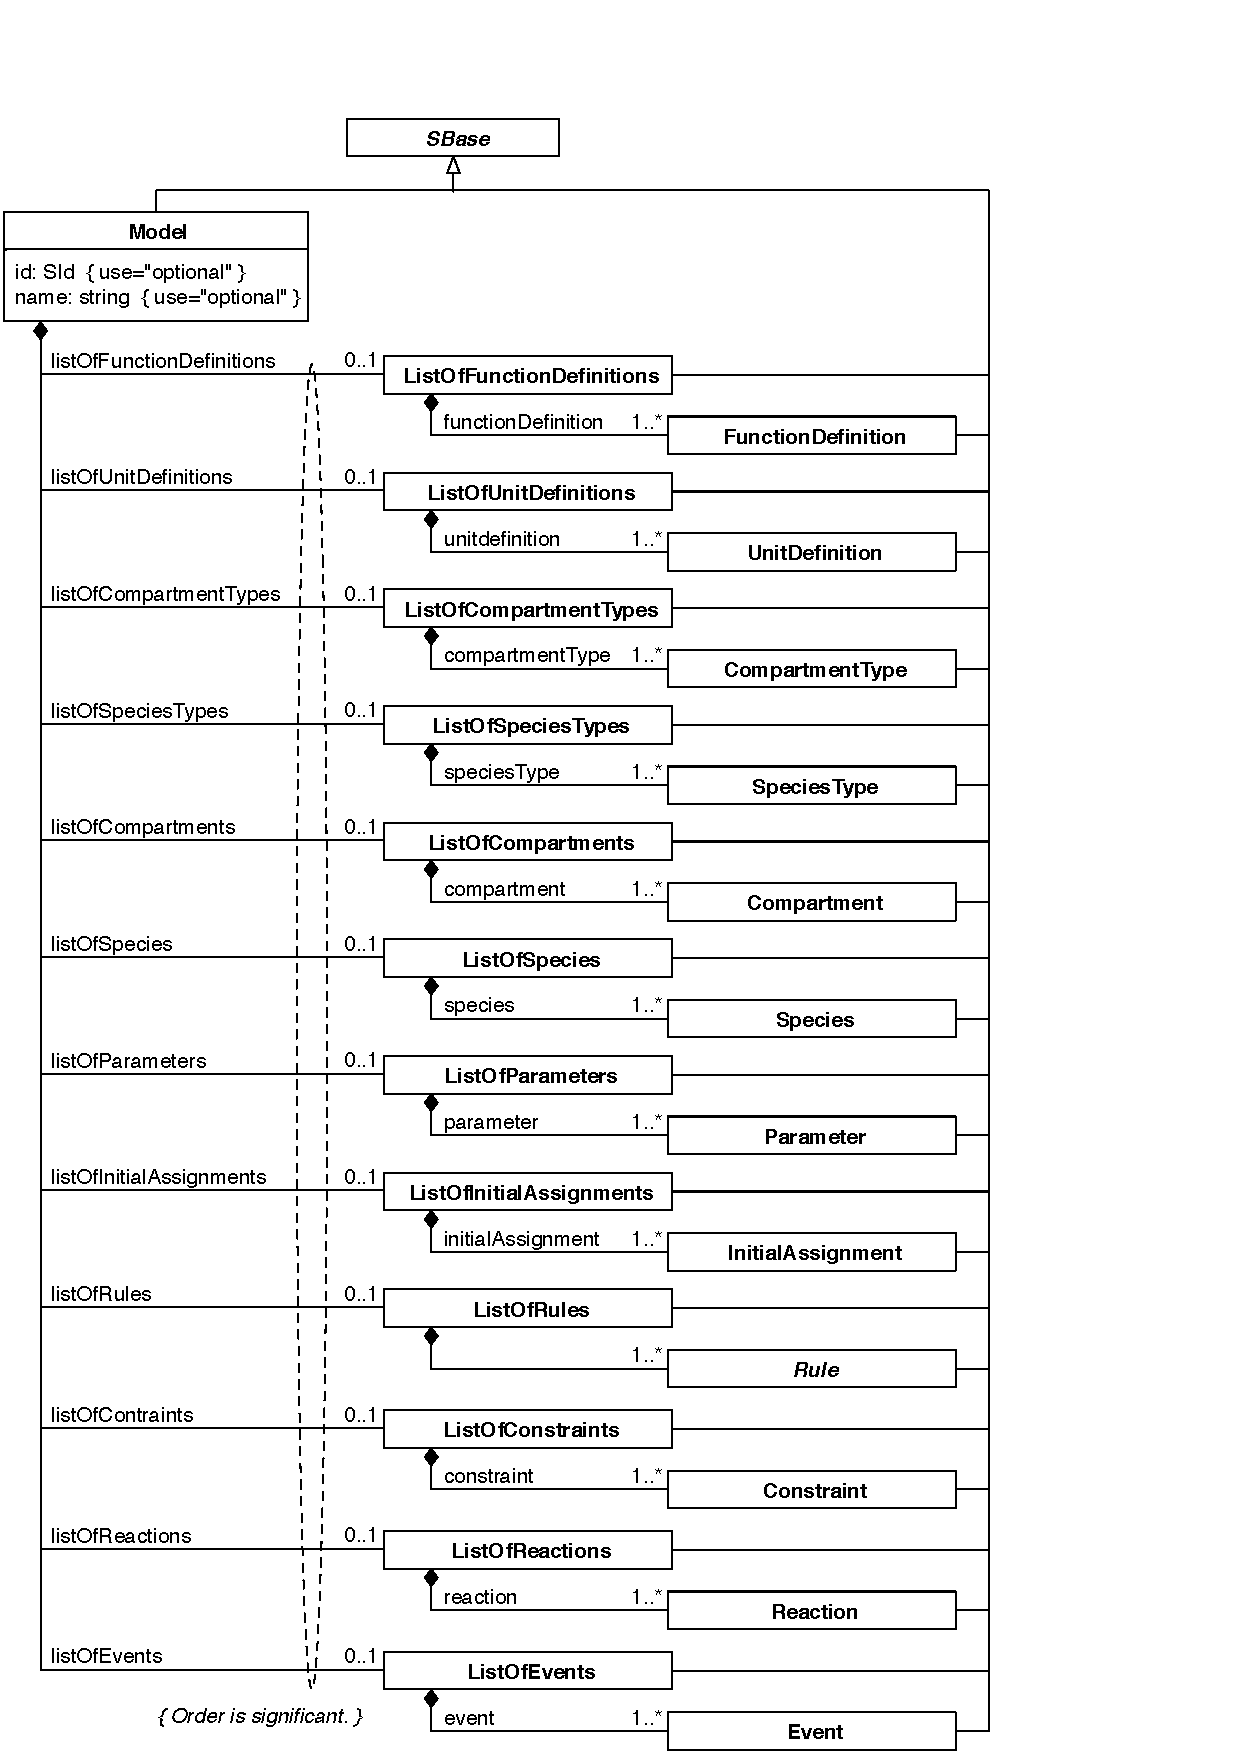
\includegraphics[scale=0.75]{figs/model-uml}
  \caption{The definition of \Model and the many helper
      classes \ListOfFunctionDefinitions, \ListOfUnitDefinitions,
      \ListOfCompartments, \ListOfSpecies, \ListOfParameters,
      \ListOfInitialAssignments, \ListOfRules, \ListOfConstraints,
      \ListOfReactions, and \ListOfEvents.}
  \label{fig:model}
\end{figure}

\Model serves as a container for components of classes
\FunctionDefinition, \UnitDefinition, \Compartment, \Species, \Parameter,
\InitialAssignment, \Rule, \Constraint, \Reaction and \Event.
Instances of the classes are placed inside instances of classes
\ListOfFunctionDefinitions, \ListOfUnitDefinitions,
\ListOfCompartments, \ListOfSpecies, \ListOfParameters, \ListOfInitialAssignments,
\ListOfRules, \ListOfConstraints, \ListOfReactions, and
\ListOfEvents.  The ``list'' classes are defined in
Figure~\ref{fig:model}.  All of the lists are optional, \changed{and if a
given list container \emph{is} present within the model, the list may
be empty; that is, it may have no children, which is semantically identical to the list being absent.}  The
resulting XML data object for a full model containing every
possible list would have the following form:

\newcommand{\sayOptional}{\raisebox{0pt}[0pt][0pt]{\bigg\} \textrm{\emph{optional}}}}

\vspace*{2ex}
\begin{tt}
  \tightspacing
  \small
  \begin{tabbing}
xxxx\=xxxx\=xxxx\=xxxx\=xxxx\=\kill
\+\>
<?xml version="1.0" encoding="UTF-8"?>\\
<sbml xmlns="http://www.sbml.org/sbml/level3/version2/core" level="3" version="2">\\
\><model id="My\_Model">\\
\>\><listOfFunctionDefinitions>\\
\>\>\>\textrm{\emph{\changed{zero} or more}} <functionDefinition> ... </functionDefinition> \textrm{\emph{elements}}  \` \sayOptional\\
\>\></listOfFunctionDefinitions>\\
\>\><listOfUnitDefinitions>\\
\>\>\>\textrm{\emph{\changed{zero} or more}} <unitDefinition> ... </unitDefinition> \textrm{\emph{elements}}  \` \sayOptional\\
\>\></listOfUnitDefinitions>\\
\>\><listOfCompartments>\\
\>\>\>\textrm{\emph{\changed{zero} or more}} <compartment> ... </compartment> \textrm{\emph{elements}}  \` \sayOptional\\
\>\></listOfCompartments>\\
\>\><listOfSpecies>\\
\>\>\>\textrm{\emph{\changed{zero} or more}} <species> ... </species> \textrm{\emph{elements}}  \` \sayOptional\\
\>\></listOfSpecies>\\
\>\><listOfParameters>\\
\>\>\>\textrm{\emph{\changed{zero} or more}} <parameter> ... </parameter> \textrm{\emph{elements}}  \` \sayOptional\\
\>\></listOfParameters>\\
\>\><listOfInitialAssignments>\\
\>\>\>\textrm{\emph{\changed{zero} or more}} <initialAssignment> ... </initialAssignment> \textrm{\emph{elements}}  \` \sayOptional\\
\>\></listOfInitialAssignments>\\
\>\><listOfRules>\\
\>\>\>\textrm{\emph{\changed{zero} or more elements of subclasses of \abstractclass{Rule}}}  \` \sayOptional\\
\>\></listOfRules>\\
\>\><listOfConstraints>\\
\>\>\>\textrm{\emph{\changed{zero} or more}} <constraint> ... </constraint> \textrm{\emph{elements}}  \` \sayOptional\\
\>\></listOfConstraints>\\
\>\><listOfReactions>\\
\>\>\>\textrm{\emph{\changed{zero} or more}} <reaction> ... </reaction> \textrm{\emph{elements}}  \` \sayOptional\\
\>\></listOfReactions>\\
\>\><listOfEvents>\\
\>\>\>\textrm{\emph{\changed{zero} or more}} <event> ... </event> \textrm{\emph{elements}}  \` \sayOptional\\
\>\></listOfEvents>\\
\></model>\\
</sbml>
\end{tabbing}
\regularspacing
\end{tt}
\vspace*{0.5ex}

Although the lists are optional, there are dependencies between
SBML components such that defining some components requires
defining others.  For example, defining a species requires
defining a compartment, and defining a \changed{species reference in a reaction} requires defining
a species.  Such dependencies are explained throughout this
document.
  

%\subsubsection{The \token{id} and \token{name} attributes}
%\label{sec:model-id}

%\changed{\Model inherits the optional attribute} \token{id}, used to
%give the model an identifier.  The value of \token{id} must
%conform to the syntax permitted by the \primtype{SId} data type
%described in Section~\ref{sec:sid}.  \Model also has an optional
%\token{name} attribute, of type \primtype{string}.  The
%\token{name} and \token{id} attributes must be used as described
%in Section~\ref{sec:idnameattribs}.


\subsubsection{The \token{sboTerm} attribute}
\label{sec:model-sboterm}

\Model inherits an optional \token{sboTerm} attribute of type
\primtype{SBOTerm} from its parent class \SBase (see
Sections~\ref{sec:sboterm-type} and~\ref{sec:sboTerm}).  When a
value is given to this attribute in a \Model instance, it should
be an SBO identifier belonging to the branch for type \Model
indicated in Table~\ref{tab:sboterm-availability}.  The
  relationship is of the form ``the model definition \emph{is-a}
  X'', where X is the SBO term.  The term chosen should be the
most precise (narrow) one that captures the overall process or
phenomenon represented by the overall SBML model.

As discussed in Section~\ref{sec:sboTerm}, SBO labels are optional
information on a model.  Applications are free to ignore
\token{sboTerm} values.  A model must be interpretable without the
benefit of SBO labels.


\subsubsection{The \token{substanceUnits} attribute}
\label{sec:model-substanceUnits}
\label{sec:substanceunits}

The \token{substanceUnits} attribute is used to specify the unit
of measurement associated with substance quantities of \Species
objects that do not specify units explicitly.  The attribute's
value must be of type \primtype{UnitSIdRef}
(Section~\ref{sec:unitsidref}).  A list of recommended units is
given in Section~\ref{sec:bp:unitdefinitions:recommendedunits}.

If a given \Species object definition does not specify its unit of
substance quantity via the \token{substanceUnits} attribute on
\Species (described in Section~\ref{sec:species}), then the
species inherits the value of the \Model \token{substanceUnits}
attribute.  If the \Model does not define a value for this
attribute, then there is no unit to inherit, and all species that
do not specify individual \token{substanceUnits} attribute values
then have \emph{no} declared units for their quantities.
Section~\ref{sec:species-substanceunits} provides more information
about the units of species quantities.

Note that when the identifier of a species appears in a model's
mathematical expressions, the unit of measurement associated with
that identifier is \emph{not solely determined} by setting
\token{substanceUnits} on \Model or \Species.
Sections~\ref{sec:species-units} and~\ref{sec:species-meaning}
explain this point in more detail.


\subsubsection{The \token{timeUnits} attribute}
\label{sec:model-timeUnits}
\label{sec:timeunits}

The \token{timeUnits} attribute is used to specify the unit in
which time is measured in the model.  The value of this attribute
must be of type \primtype{UnitSIdRef}
(Section~\ref{sec:unitsidref}).  A list of recommended units is
given in Section~\ref{sec:bp:unitdefinitions:recommendedunits}.

This attribute on \Model is the \emph{only} way to specify a unit
for time in a model.  It is a global attribute; time is measured
in the model everywhere in the same way.  This is particularly
relevant to \Reaction and \RateRule objects in a model: all
\Reaction and \RateRule objects in SBML define per-time values,
and the unit of time is given by the \token{timeUnits} attribute
on the \Model object instance.  If the \Model \token{timeUnits}
attribute has no value, it means that the unit of time is not
defined for the model's reactions and rate rules.  Leaving it
unspecified in an SBML model does not result in an invalid model;
however, as a matter of best practice, we strongly recommend that
all models specify units of measurement for time.


\subsubsection{The \token{volumeUnits}, \token{areaUnits} and
  \token{lengthUnits} attributes}
\label{sec:model-volumeUnits}
\label{sec:model-areaUnits}
\label{sec:model-lengthUnits}
\label{volumeunits}
\label{areaunits}
\label{lengthunits}

The attributes \token{volumeUnits}, \token{areaUnits} and
\token{lengthUnits} together are used to set the units of
measurements for the sizes of \Compartment objects in the model
when those objects do not otherwise specify units.  The three
attributes correspond to the most common cases of compartment
dimensions: \token{volumeUnits} for compartments having attribute
value \token{spatialDimensions}=\val{3}, \token{areaUnits} for
compartments having \token{spatialDimensions}=\val{2}, and
\token{lengthUnits} for compartments having
\token{spatialDimensions}=\val{1}.  The values of these attributes
must be of type \primtype{UnitSIdRef}
(Section~\ref{sec:unitsidref}).  A list of recommended units is
given in Section~\ref{sec:bp:unitdefinitions:recommendedunits}.
The attributes are not applicable to compartments whose
\token{spatialDimensions} attribute values are not one of \val{1},
\val{2} or \val{3}.

If a given \Compartment object instance does not provide a value
for its \token{units} attribute, then the unit of measurement of
that compartment's size is inherited from the value specified by
the \Model \token{volumeUnits}, \token{areaUnits} or
\token{lengthUnits} attribute, as appropriate based on the
\Compartment object's \token{spatialDimensions} attribute value.
If the \Model object does not define the relevant attribute, then
there are no units to inherit, and all compartments that do not
set a value for their \token{units} attribute then have \emph{no}
units associated with their compartment sizes.
Section~\ref{sec:compartment-units} provides more information
about units of compartment sizes.

The use of three separate attributes is a carry-over from SBML
Level~2.  Note that it is entirely possible for a model to define
a value for two or more of the attributes \token{volumeUnits},
\token{areaUnits} and \token{lengthUnits} simultaneously, because
SBML models may contain compartments with different numbers of
dimensions.


\subsubsection{The \token{extentUnits} attribute}
\label{sec:model-extentUnits}
\label{extentunits}

Reactions are processes that occur over time.  These processes
involve events of some sort, where a single ``reaction event'' is
one in which some set of entities (known as reactants, products
and modifiers in SBML) interact, once.  The \emph{extent} of a
reaction is a measure of how many times the reaction has occurred,
while the time derivative of the extent gives the instantaneous
rate at which the reaction is occurring.  Thus, what is
colloquially referred to as the ``rate of the reaction'' is in
fact equal to the rate of change of reaction extent.

The combination of \token{extentUnits} and \token{timeUnits}
defines the units of kinetic laws in SBML and establishes how the
numerical value of each \KineticLaw's mathematical formula
(Section~\ref{subsec:kinetic-law}) is meant to be interpreted in a
model.  The units of the kinetic laws are taken to be
\token{extentUnits} divided by \token{timeUnits}.  A list of
recommended units is given in
Section~\ref{sec:bp:unitdefinitions:recommendedunits}.

Note that this embodies an important principle in SBML models:
\emph{all reactions in an SBML model must have the same units} for
the rate of change of extent.  In other words, the units of all
reaction rates in the model \emph{must be the same}.  There is
only one global value for \token{extentUnits} and one global value
for \token{timeUnits}.


\subsubsection{The \token{conversionFactor} attribute}
\label{sec:model-conversionFactor}

The attribute \token{conversionFactor} defines a global value
inherited by all \Species object instances that do not define
separate values for their \token{conversionFactor} attributes.  The
value of this attribute must be of type \primtype{SIdRef}
(Section~\ref{sec:sidref}) and refer to a \Parameter object
instance defined in the model.  The \Parameter object in question
must be a constant; \ie it must have its \token{constant}
attribute value set to \val{true}.

If a given \Species object definition does not specify a
conversion factor via the \token{conversionFactor} attribute on
\Species (described in Section~\ref{sec:species}), then the
species inherits the conversion factor specified by the \Model
\token{conversionFactor} attribute.  If the \Model does not define
a value for this attribute, then there is no conversion factor to
inherit.  Section~\ref{sec:about-kinetic-laws} describes how to
interpret the effects of reactions on species in that situation.
More information about conversion factors in SBML is provided in
Sections~\ref{sec:species} and~\ref{sec:reactions}.


\subsubsection{The ListOf container classes}
\label{sec:listof}
\label{sec:listofunitdefinitions}
\label{sec:listoffunctiondefinitions}
\label{sec:listofcompartments}
\label{sec:listofspecies}
\label{sec:listofparameters}
\label{sec:listofinitialassignments}
\label{sec:listofinitialassign}
\label{sec:listofrules}
\label{sec:listofconstraints}
\label{sec:listofreactions}
\label{sec:listofevents}

The various \ListOf classes defined in Figure~\ref{fig:model} are
merely containers used for organizing the main components of an
SBML document.  \ListOfFunctionDefinitions,
\ListOfUnitDefinitions, \ListOfCompartments, \ListOfSpecies,
\ListOfParameters, \ListOfInitialAssignments, \ListOfRules,
\ListOfConstraints, \ListOfReactions, and \ListOfEvents are all
derived from the abstract class \SBase (Section~\ref{sec:sbase}),
and inherit \SBase's various attributes and subelements.  The
\ListOf classes do not add any attributes of their own.

There are several motivations for grouping SBML components within
XML elements with names of the form \token{listOfClassNames}
rather than placing all the components directly at the top level.
First, the fact that the container classes are derived from \SBase
means that software tools can add information about the lists
themselves into each list container's \Annotation, a feature that
a number of today's software tools exploit.  Second, we believe
the grouping leads to a more modular structure that is helpful
when working with elements from multiple SBML Level~3 packages.
Third, we believe that it makes visual reading of models in XML
easier, for situations when humans must inspect and edit SBML
directly.

\begin{blockChanged}
Lists are allowed to be empty for two reasons.  First, this design allows modelers to add \Annotation and \Notes objects to a given list even when the list is empty in a model; this can be useful, for instance, to let the modeler explain \emph{why} the components are absent from the model.  Second, it enables SBML Level~3 package specifications to define new elements to be children of these lists, and for these child elements to be used without the requirement that at least one SBML Level~3 Core element always be present.
\end{blockChanged}

%-----------------------------------------------------------------------------
\subsection{Function definitions}
\label{sec:functiondefinition}
%-----------------------------------------------------------------------------

The \FunctionDefinition object associates an identifier with a
function definition.  This identifier can then be used as the
function called in subsequent MathML \token{apply} elements.
\FunctionDefinition is shown in Figure~\ref{fig:mathdefinition}.

\begin{figure}[htb]
  \centering
  \small
  \vspace*{-0.75ex}
  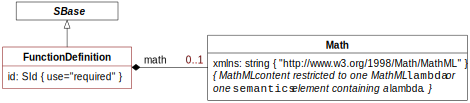
\includegraphics[scale=0.78]{figs/functiondefinition-uml}
  \vspace*{-1ex}
  \caption{The definition of class \FunctionDefinition.  A
    \class{Lambda} class object must contain a single \mathml
    \token{lambda} expression (or a \token{lambda} surrounded by a
    \token{semantics} element).  A function definition \changed{may}
    contain \changed{no more than} one \token{math} element defined by the
    \class{Lambda} class, \changed{plus a boolean \token{isRecursive} attribute}.  Note also that \class{Lambda} is not
    derived from \SBaseUpright, which means that the attributes defined
    on \SBaseUpright are \emph{not} available on the \token{math}
    element.  A sequence of \changed{zero} or more instances of
    \FunctionDefinition objects can be located in an instance of
    \ListOfFunctionDefinitions in \Model, as shown in
    Figure~\protect\ref{fig:model}.}
  \label{fig:mathdefinition}
  \label{fig:functionDefinition}
\end{figure}

Function definitions in SBML (also informally known as
``user-defined functions'') have purposefully limited capabilities.
As is made clearer below, a function cannot reference
parameters or other model quantities outside of itself; values
must be passed as parameters to the function.  Moreover, recursive
and mutually-recursive functions are \changed{permitted only if the value of the \token{isRecursive} attribute is set to \val{true}}.  The purpose
of these limitations is to balance power against complexity of
implementation.  With the restrictions as they are, function
definitions could, if desired, be implemented as textual substitutions.
Software implementations therefore do not need
the full function-definition machinery typically associated with
programming languages.


\subsubsection{The \token{id} attribute}

\begin{blockChanged}
\FunctionDefinition inherits the \token{id} attribute from \SBase, but defines \token{id} as being required rather than optional.  The \token{id} attribute otherwise obeys the behavior described in Section~\ref{sec:idnameattribs}.  A function's identifier can be used in \token{math} elements as the first target of an \token{apply} element, but has no value associated with it, and may not be the target of an \InitialAssignment, \EventAssignment, or \Rule.
\end{blockChanged}


\begin{blockChanged}
\subsubsectionChanged{The \token{isRecursive} attribute}

The \token{isRecursive} attribute is of type \primtype{boolean}, and indicates whether the \FunctionDefinition is recursive or not.  If the \FunctionDefinition's child \class{Lambda} element refers to itself, either directly or indirectly, this attribute must be set \val{true}.  Otherwise, it may be set \val{false}.

Recursive functions must terminate, as through the use of a \token{piecewise} function.  However, it is not always possible to determine this through a validation analysis.  A simulator may therefore need to break a cascade of recursive functions arbitrarily in the middle of a simulation.  If this happens, the simulator should indicate that this has occurred, and may proceed, or not, as seems fit.  It is incorrect for a simulator to break recusion arbitrarily and continue without at least indicating that the infinite recursion occurred.
\end{blockChanged}


\subsubsectionChanged{The \token{math} element}
\label{sec:function-definition-math}

The \changed{optional} \token{math} element is a container for MathML content that
defines the function.  The content of this element can only be a
MathML \token{lambda} element or a MathML \token{semantics}
element containing a \token{lambda} element.  \FunctionDefinition
is the only place in SBML Level~3 Core where a \token{lambda}
element can be used.  \changed{If present,} the \token{lambda} element must begin with
zero or more \token{bvar} elements, followed by any other of the
elements in the MathML subset listed in
Section~\ref{sec:mathmlsubset} \emph{except} \token{lambda} (\ie a
\token{lambda} element cannot contain another \token{lambda}
element).

A further restriction on the content of \token{math} is it cannot
contain references to identifiers other than the
\changed{symbols} declared in the \token{lambda} itself.  That
is, the contents of MathML \token{ci} elements inside the body of
the \token{lambda} can only be one of three kinds of
  identifiers: (i) the \changed{symbols} declared by its \token{bvar}
  elements, (ii) the identifiers of other
\FunctionDefinition objects defined in the same model,
\changed{or (iii) its own identifier (if the \token{isRecursive} attribute is set to \val{true}).}
This
restriction also applies to the \token{csymbol} elements for
\quantity{time}, \quantity{avogadro}, \quantity{delay}, \changed{ and \quantity{rateOf}}.
Functions must be written so that all model \changed{symbols} they use are
passed to them via their parameters.

\changed{If the \token{math} element is not present in the \FunctionDefinition, the function has no mathematical meaning defined in SBML core.  A meaning may be provided by means of a package or custom annotation, but any interpreter that only understands core SBML will not be able to derive that meaning.}


\subsubsectionChanged{The \token{sboTerm} attribute}
\label{sec:functiondefinition-sboterm}

\FunctionDefinition inherits an optional \token{sboTerm}
attribute of type \primtype{SBOTerm} from its parent
class \SBase (see Sections~\ref{sec:sboterm-type}
and~\ref{sec:sboTerm}).  When a value is given to this
attribute in a \FunctionDefinition instance, it should be an
SBO identifier belonging to the branch for type \FunctionDefinition 
indicated in Table~\ref{tab:sboterm-availability}.  The relationship is
of the form ``the function definition \emph{is-a} X'', where X is
the SBO term.  The term chosen should be the most precise (narrow)
one that captures the role of the function in the model.

As discussed in Section~\ref{sec:sboTerm}, SBO labels are optional
information on a model.  Applications are free to ignore
\token{sboTerm} values.  A model must be interpretable without the
benefit of SBO labels.


\subsubsectionChanged{Calling user-defined functions}
\label{sec:functiondefinition-calling}

Within MathML expressions in an SBML model, all calls to a
function defined by a \FunctionDefinition must use the same number
of arguments as specified in the function's definition, \changed{if present}.  The
number of arguments is equal to the number of \token{bvar}
elements inside the \token{lambda} element of the function
definition.  \changed{If the \FunctionDefinition has no \token{math} child, no restriction is placed, in core, on the number of arguments the function may take when used in MathML elsewhere in the model.  Without further information (such as might be supplied by a package), however, the call will be mathematically meaningless.}

Note that \FunctionDefinition does not have a separate attribute
for defining the unit of measurement associated with the value
returned by the function.  The unit is taken to be whatever
results from evaluating the expression when the
\FunctionDefinition's \token{math} is applied to the arguments
supplied in the call to that function.  (See also
Section~\ref{sec:unit-consistency}.)


\subsubsectionChanged{Examples}

The following abbreviated SBML example shows a \FunctionDefinition
object instance defining \token{pow3} as the identifier of a function
computing the mathematical expression $x^{3}$, and after that, the
invocation of that function in the mathematical formula of a rate
law.  Note how the invocation of the function uses its identifier.

\begin{example}
<model ...>
   <listOfFunctionDefinitions>
       <functionDefinition id="pow3">
           <math xmlns="http://www.w3.org/1998/Math/MathML"
                 xmlns:sbml="http://www.sbml.org/sbml/level3/version2/core">
               <lambda>
                   <bvar><ci> x </ci></bvar>
                   <apply> <power/> <ci> x </ci> <cn sbml:units="dimensionless"> 3 </cn> </apply>
               </lambda>
           </math>
       </functionDefinition>
   </listOfFunctionDefinitions>
   ...
   <listOfReactions>
       <reaction id="reaction_1" reversible="true" fast="false">
           ...
           <kineticLaw>
               <math xmlns="http://www.w3.org/1998/Math/MathML">
                   <apply> <ci> pow3 </ci> <ci> S1 </ci> </apply>
               </math>
           </kineticLaw>
           ...
       </reaction>
   </listOfReactions>
   ...
</model>\end{example}


%-----------------------------------------------------------------------------
\subsection{Unit definitions}
\label{sec:unitdefinitions}
%-----------------------------------------------------------------------------

The unit of measurement associated with the value produced by a
mathematical formula is whatever arises naturally from the
components and mathematical expressions comprising the formula, or
in other words, the unit obtained by doing dimensional analysis on
the formula.  To support this, units may be supplied in a number
of contexts in an SBML model and associated with a variety of
components, and SBML provides a facility for defining units that
can be reused and referenced throughout a model.  The unit
definition facility uses two classes of objects, \UnitDefinition
and \Unit.  Their definitions are shown in
Figure~\vref{fig:unitdefinition} and explained in more detail
below.

Before delving further into the definition of SBML units, we must
highlight two important and sometimes-confusing points.  First,
unit declarations in SBML models are \emph{optional}.  The
consequence of this is that a model must be numerically
self-consistent independently of unit declarations, for the
benefit of software tools that cannot interpret or manipulate
units.  Unit declarations in SBML are thus more akin to a type of
annotation; they can indicate intentions, and can be used by model
readers for checking the consistency of the model, labeling
simulation output, etc., but any transformations of values implied
by different units must be incorporated \emph{explicitly} into a
model.  We revisit this topic in Section~\ref{sec:using-units},
and illustrate it again with the example given in
Section~\ref{sec:eg:conversionfactor}.

Second, the vast majority of situations that require new SBML unit
definitions involve simple multiplicative combinations of base
units and factors.  An example is ``moles per litre per second''.
What distinguishes these sorts of unit definitions from more
complex ones is that they may be expressed without the use of an
additive offset from a zero point.  The use of offsets complicates
all unit definition systems, yet in the domain of SBML, the
real-life cases requiring offsets are few (and in fact, to the
best of our knowledge, only involve temperature).  Consequently,
the SBML unit system has been consciously designed to simplify
implementation of unit support for the most common cases in
systems biology.  The cost of this simplification is to require
units with offsets to be handled explicitly by the modeler.
Section~\ref{sec:bp:unitdefinitions:offset} discusses approaches
for handling situations requiring units with offsets.


\subsubsection{\class{UnitDefinition}}
\label{sec:unitdefinition-structure}

The approach to defining units in SBML is compositional; for
example, $metre\ second^{\,-2}$ is constructed by combining a
\Unit object representing $metre$ with another \Unit object
representing $second^{\,-2}$.  The combination is wrapped inside a
\UnitDefinition, which provides for assigning an identifier and
optional name to the combination.  These object classes are
defined in Figure~\ref{fig:unitdefinition}.  Once a unit is
defined using a \UnitDefinition object, it can then be referenced
from elsewhere in a model.

\begin{figure}[htb]
  \centering
  \vspace*{1ex}
  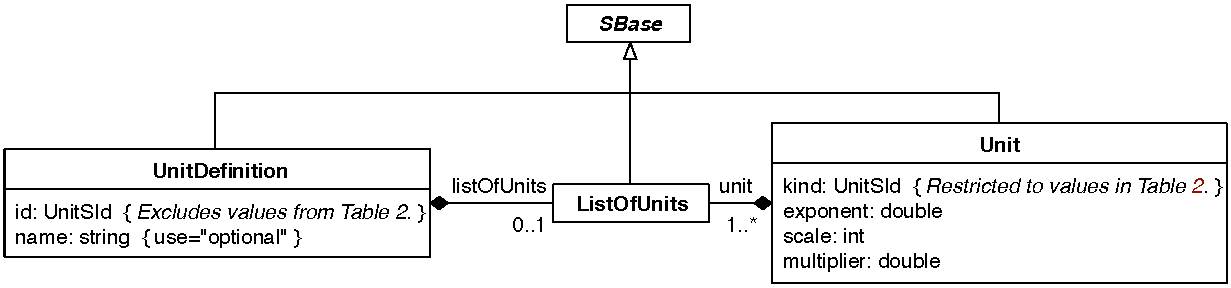
\includegraphics[scale=0.78]{figs/unitdefinition-uml}
  \caption{The definition of classes \UnitDefinition and
      \Unit.  A sequence of \changed{zero} or more instances of
      \UnitDefinition can be located in an instance of
      \ListOfUnitDefinitions in \Model
      (Figure~\protect\ref{fig:model}).  \ListOfUnits has
      no attributes (beyond those it inherits from class \SBaseUpright);
      it merely acts as a container for \changed{zero} or more instances of
      \Unit objects.  Note that the only permitted values of
      \token{kind} on \Unit are the reserved words in
      Table~\vref{tab:unitkind}, but these symbols are
      \emph{excluded} from the permitted values of
      \UnitDefinition's \token{id} because SBML's unit system does
      not allow redefining the base units.}
  \label{fig:unitdefinition}
\end{figure}


\paragraphChanged{The \token{id} attribute}

\begin{blockChanged}
\UnitDefinition inherits the \token{id} attribute from \SBase, but defines \token{id} as being required rather than optional, and in addition, refines the data type of \token{id} to be  \primtype{UnitSId} instead of \primtype{SId}.  This is done to provide each unit definition with a unique identifier by which other parts of a model may refer to it; see Section~\ref{sec:idnameattribs} for more details.
\end{blockChanged}

There is one important restriction about the use of unit
definition \token{id} values: the \token{id} of a \UnitDefinition
must \emph{not} be equal to one of the reserved base unit
  names listed in Table~\ref{tab:unitkind}, the list of reserved
base unit names.  This constraint simply prevents the redefinition
of base units.


\paragraph{The list of \class{Unit}s}
\label{sec:listofunits}

A \UnitDefinition object may contain a \ListOfUnits container which \changed{may
contain zero or more} \Unit objects. Section~\ref{sec:unit-structure} explains
the meaning and use of \Unit.   

\paragraph{Example}

The following skeleton of a unit definition illustrates an example
use of \UnitDefinition:

\begin{example}
<model ...>
    <listOfUnitDefinitions>
        <unitDefinition id="unit1">
            <listOfUnits>
                ...
            </listOfUnits>
        </unitDefinition>
        <unitDefinition id="unit2">
            <listOfUnits>
                ...
            </listOfUnits>
        </unitDefinition>
    </listOfUnitDefinitions>
    ...
</model>
\end{example}


\subsubsection{\class{Unit}}
\label{sec:unit-structure}

A \Unit object represents a reference to a (possibly transformed)
base unit chosen from the list in Table~\vref{tab:unitkind}.  The
attribute \token{kind} indicates the base unit, whereas the
attributes \token{exponent}, \token{scale}, and \token{multiplier}
define how the base unit is being transformed.  The attributes
are described in detail below.


\paragraph{The \token{kind} attribute}

The \Unit attribute \token{kind} specifies a base unit to serve as
the starting point for a new unit definition.  The value of the
attribute must be taken from the list of reserved words given in
Table~\vref{tab:unitkind}.  These reserved symbols are defined in
the value space of the data type \primtype{UnitSId}
(Section~\ref{sec:unitsid}).

\begin{table}[bht]
  \vspace*{1em}
  \centering
  \ttfamily
  \small
  \setlength{\arraycolsep}{8pt}
  \begin{edtable}{tabular}{@{}llllll@{}}
    \toprule
    ampere                    & farad            & joule    & lux      & radian    & volt  \\
    \underline{avogadro}      & gram             & katal    & metre    & second    & watt  \\
    becquerel                 & gray             & kelvin   & mole     & siemens   & weber \\
    candela                   & henry            & kilogram & newton   & sievert           \\
    coulomb                   & hertz            & litre    & ohm      & steradian         \\
    \underline{dimensionless} & \underline{item} & lumen    & pascal   & tesla             \\
    \bottomrule
  \end{edtable}
  \caption{Base units defined in SBML.  These symbols are
    predefined values of type \primtype{UnitSId}
    (Section~\ref{sec:unitsid}).  All are names of base or derived
    SI units~\protect\citep{bipm:2006}, except for
    ``\token{avogadro}'', ``\token{dimensionless}'' and
    ``\token{item}'', which are SBML additions.  The unit
    ``\token{dimensionless}'' is intended for cases where a
    quantity is a ratio whose units cancel out, the unit
    ``\token{avogadro}'' is the unit ``\token{dimensionless}''
    multiplied with Avogadro's number, 
    and ``\token{item}'' is used for expressing such things as 
    ``N items'' when ``mole'' is not an appropriate unit.   The
    gram and litre are not strictly part of SI; however, they are
    frequently used in SBML's areas of application and therefore
    are included as predefined unit identifiers.  (The standard SI
    unit of mass is the kilogram, and  volume in SI is defined in
    terms of cubic metres.)  Comparisons of these values, like all
    values of type \primtype{UnitSId}, must be performed in a
    case-sensitive manner.}
  \label{tab:unitkind}
\end{table}

Note that the set of acceptable values for the attribute
\token{kind} does \emph{not} include units defined by
\UnitDefinition objects.  This means that the unit definition
system in SBML is not hierarchical: user-defined units cannot be
built on top of other user-defined units, only on top of base
units.

The presence of \token{avogadro} in Table~\ref{tab:unitkind}
warrants an explanation.  The Bureau International des Poids et
Mesures specifically states, ``When the mole is used, the
elementary entities must be specified and may be atoms, molecules,
ions, electrons, other particles, or specified groups of such
particles''~\cite[p.~115]{bipm:2006}---in other words, the SI unit
\token{mole} is technically \emph{a unit of measure for substance
  amount}.  Although people sometimes use ``mole'' loosely to
refer to other things besides substance amounts (\eg ``a mole of
\emph{X}'' to mean a number of \emph{X} equal to Avogadro's
number, $6.022 \cdot 10^{23}$), such usage is not strictly
correct.  We believe it is even less correct in the context of
reactions: although in SBML they are called ``reactions'', there
is nothing preventing the SBML \Reaction construct from being used
to represent other kinds of processes not involving substances.
Consequently, we avoid using \val{mole} loosely where substances
may not be involved, and instead use ``Avogadro's number of
\emph{X}''.  In order to make it easier for models to define units
in these terms, the SBML unit system includes the pseudo-unit
\val{avogadro}, whose definition is identical to the definition of
the \emph{avogadro} \token{csymbol} described in
Section~\ref{sec:csymbol}.  The numerical value is taken to be the
one recommended by CODATA~\citep{codata_2008}, but the unit is
\token{dimensionless}.  In other words, it is defined as
\begin{linenomath}
  \begin{equation*}
    (6.02214179 \cdot 10^{23}) \cdot \textrm{\texttt{dimensionless}}
  \end{equation*}
\end{linenomath}
where the dot ($\cdot$) indicates simple scalar multiplication.
If the value of Avogadro's constant is revised by international
standards-setting organizations in the future, a future Version of
the SBML \thisL specification may stipulate a new value to be used
for \token{avogadro}.  However, all software reading models
expressed in \emph{this} version of SBML Level~3 should
\emph{always} use the value of Avogadro's constant given above.

Software tools must use identical numerical values of Avogadro's
constant for both the base unit \token{mole} and the unit \token{avogadro}.


\paragraph{The \token{exponent}, \token{scale} and
  \token{multiplier} attributes}
\label{sec:unit-structure:exponent}
\label{sec:unit-structure:scale}
\label{sec:unit-structure:multiplier}

\newcommand{\ynew}{\ensuremath{y}\xspace}
\newcommand{\ybase}{\ensuremath{y_b}\xspace}
\newcommand{\udef}{\ensuremath{u}\xspace}
\newcommand{\unew}{\ensuremath{u_\text{new}}\xspace}
\newcommand{\ubase}{\ensuremath{u_b}\xspace}
\newcommand{\ukind}{\ensuremath{u_\tokenNC{\,kind}}\xspace}
\newcommand{\uone}{\ensuremath{u_{b_1}}\xspace}
\newcommand{\utwo}{\ensuremath{u_{b_2}}\xspace}
\newcommand{\un}  {\ensuremath{u_{b_n}}\xspace}

The attributes \token{exponent}, \token{scale} and
\token{multiplier} work together to permit the use of \Unit for
expressing new units in terms of the base units listed in
Table~\vref{tab:unitkind}.  The formula underlying this definition
is the following:
\begin{linenomath}
\begin{equation}
  \unew = (\textrm{\tokenNC{multiplier}} \cdot 10^\textrm{\tokenNC{scale}} \cdot \ukind)^\textrm{\tokenNC{exponent}}
\label{eq:unit-semantics}
\end{equation}
\end{linenomath}

This formula defines a new unit, \unew, in terms of another unit,
\ukind.  The unit \ukind is one of the units listed in
Table~\ref{tab:unitkind}; in a given \Unit object, it is
chosen by setting the \token{kind} attribute.  Each of the other
components on the right-hand side of
Equation~\ref{eq:unit-semantics} corresponds to the remaining
attributes in a \Unit object instance, and their meanings are as
follows:
\begin{itemize}

\item The \token{multiplier} attribute can be used to multiply the
  \token{kind} unit by a real-numbered factor.  This enables the
  definition of units that are not power-of-ten multiples of SI
  units.  For instance, a \token{multiplier} of 0.3048 could be
  used to define \val{foot} as a measure of length in terms of a
  \val{metre}.  A value of \token{multiplier} must always be
  provided in a \Unit object instance, but the value can be
  \val{1}.

\item The \token{scale} attribute can be used to set the exponent
  for a power-of-ten multiplier that rescales the unit.  For
  example, a unit having a \token{kind} value of \val{gram} and a
  \token{scale} value of \val{-3} signifies $10^{-3} \cdot gram$,
  or milligrams.  In those cases where a unit does not need to be
  scaled by a power of ten, the value of \token{scale} can be set
  to \val{0} (zero), because $10^0 = 1$.

\item The \token{exponent} attribute can be used to specify an
  overall exponent on the unit definition.  This provides a way to
  define units such as ``cubic metre'' in terms of the base unit
  \val{metre} (for which an \token{exponent} value of~\val{3}
  would be appropriate).  A value of \token{exponent} must always
  be provided.

\end{itemize}


\subsubsection{Semantics of \class{Unit} and \class{UnitDefinition}}
\label{sec:unit-structure:semantics}

A single \Unit object instance takes one of the base units from
Table~\ref{tab:unitkind} and specifies how it should be
transformed.  A \UnitDefinition object instance combines one or
more \Unit objects to define a new, composed unit, \udef.  The new
unit \udef created by a \UnitDefinition is defined as the product
of all the \Unit objects contained in the \ListOfUnits within the
\UnitDefinition object instance.  More formally, 
\begin{linenomath}
\begin{equation}
  \udef = u_1 \, \cdot \, u_2 \, \cdot \ldots \cdot \, u_n 
\label{eq:unitDefinition-semantics}
\end{equation}
\end{linenomath}
where the $\{u_i\}$'s are individual \Unit definitions as defined
by Equation~\ref{eq:unit-semantics}.  Now, let the value of the
\token{multiplier} attribute of a given unit $\{u_i\}$ be
represented by the \changed{symbol} $m_i$.  Similarly, let the value of
the \token{scale} attribute be represented by $s_i$, and the value
of the \token{exponent} attribute be represented by $x_i$.
Equation~\ref{eq:unitDefinition-semantics} can be rewritten in
expanded form as
\begin{linenomath}
\begin{align}
  u &= (m_1 \cdot 10^{s_1} \cdot \uone)^{x_1} \cdot
       (m_2 \cdot 10^{s_2} \cdot \utwo)^{x_2} \cdot \ldots \cdot (m_n \cdot
       10^{s_n} \cdot \un)^{x_n} \notag \\[2pt]
    &= m_1^{x_1} \cdot m_2^{x_2} \cdot \ldots \cdot m_n^{x_n}
       \cdot 10^{(s_1 x_1 + s_2 x_2 + \ldots + s_n x_n)}
       \cdot \uone^{x_1} \cdot \utwo^{x_2} \cdot \ldots \cdot \un^{x_n} \notag \\[2pt]
    &= m \cdot 10^{s} \cdot \uone^{x_1} \cdot \utwo^{x_2} \cdot \ldots \cdot \un^{x_n}
\label{eq:multip-units}
\end{align}
\end{linenomath}
where the terms $m$ and $s$ in the last line
(Equation~\ref{eq:multip-units}) are defined as
\begin{larray*}
  m &=& m_1^{x_1} \cdot m_2^{x_2} \cdot \ldots \cdot m_n^{x_n} \\
  s &=& s_1 x_1 + s_2 x_2 + \ldots + s_n x_n
\end{larray*}
Equation~\ref{eq:multip-units} expresses how a \UnitDefinition
object instance combines multiple \Unit object instances to
produce a new unit definition in an SBML model.


\paragraph{Examples}

As a concrete example to illustrate the definitions above, let us
define a unit for \val{foot} in terms of the base unit
\val{metre}.  This requires using \token{multiplier}=\val{0.3048},
\token{scale}=\val{0}, and \token{exponent}=\val{1}:
\begin{linenomath}
\begin{equation*}
  \text{foot} = 0.3048 \cdot 10^0 \cdot \textrm{\token{metre}}
\end{equation*}
\end{linenomath}
The following fragment of SBML illustrates how this could be
represented in XML:

\begin{example}
<listOfUnitDefinitions>
    <unitDefinition id="foot">
        <listOfUnits>
            <unit kind="metre" multiplier="0.3048" scale="0" exponent="1"/>
        </listOfUnits>
    </unitDefinition>
</listOfUnitDefinitions>
\end{example}

To give another example, the following illustrates the definition
of an abbreviation \val{mmls} for the unit $millimoles\ l^{-1}\
s^{-1}$:

\begin{example}
<listOfUnitDefinitions>
    <unitDefinition id="mmls">
        <listOfUnits>
            <unit kind="mole"   exponent="1"  scale="-3" multiplier="1"/>
            <unit kind="litre"  exponent="-1" scale="0"  multiplier="1"/>
            <unit kind="second" exponent="-1" scale="0"  multiplier="1"/>
        </listOfUnits>
    </unitDefinition>
</listOfUnitDefinitions>
\end{example}

Section~\ref{sec:bp:unitdefinitions:offset} provides suggestions
for possible ways of handling cases that involve offsets, which
happen in particular with temperature measurements.


\subsubsection{Use of units in a model}
\label{sec:using-units}

As already mentioned, unit declarations are optional in SBML.
This design decision was a consensus choice among SBML developers
and users, driven by the exigencies of non-commercial software
development and the realities of models found in existence.  It
has an important and possibly counterintuitive implication that
must be kept in mind when writing and interpreting SBML models:
units associated with quantities \emph{do not alter the numerical
  interpretation} of those quantities.

An example may help make this more clear.  We know that one metre
equals 1000 millimetres:
\begin{linenomath}
  \begin{equation*}
    1\, m = 1000\, mm
  \end{equation*}
\end{linenomath}
However, the equality above relies on interpreting the units on
both sides, and taking the ``1'' and ``1000'' to be dimensionless.
If readers ignored unit labels altogether or were unable to
process them, they would see
\begin{linenomath}
  \begin{equation*}
    1 = 1000
  \end{equation*}
\end{linenomath}
which is obviously incorrect.  In an SBML model, the necessary
factor must be included explicitly, even if it is part of the
definition of the unit.  A ramification of this is that units
attached to SBML quantities must be viewed as a kind of
independent annotation or label that does not enter into the
numerical interpretation of the actual quantity or the
mathematical formulas appearing in a model.  In the present simple
formula, an explicit factor such as the following needs to be
inserted (and here we put unit names in \{$\,$\} braces to
indicate they are annotations that do not enter into the
mathematics):
\begin{linenomath}
  \begin{equation}\label{eq:factor}
    1 \, \{m\} = 1000 \cdot \frac{1 \, \{m\}}{1000 \, \{mm\}} \, \{mm\}
  \end{equation}
\end{linenomath}
This is despite the fact that a unit definition for millimetres in SBML
would take the following form:
\begin{example}
<listOfUnitDefinitions>
    <unitDefinition id="millimetre">
        <listOfUnits>
            <unit kind="metre" exponent="1" scale="-3" multiplier="1"/>
        </listOfUnits>
    </unitDefinition>
</listOfUnitDefinitions>
\end{example}

In other words, the definition \emph{also} includes a factor of
$1/1000$.  While the result is that information is duplicated
between the definition of \token{millimetre} above and the
explicit factor inserted into Equation~\ref{eq:factor}, the
machinery provided by \UnitDefinition is still necessary in order
to allow units themselves to be properly defined.  The result is
still useful and powerful: it permits software tools to check the
consistency of a model, perform unit conversions, label numbers in
the outputs of simulations, and so on.


%-----------------------------------------------------------------------------
\subsection{Compartments}
\label{sec:compartments}
%-----------------------------------------------------------------------------

A \emph{compartment} in SBML represents a bounded space in which
species are located.  Compartments do not necessarily have to
correspond to actual structures inside or outside of a biological
system, although models are often designed that way.  The definition
of \Compartment is shown in Figure~\vref{fig:compartment}.

\begin{figure}[htb]
  \centering
  \small
  \begin{tikzpicture}
    \node[above=0.9in] (a) {
      \emptyClassbox{\textsl{SBase}}
    };
    \node (b) {
      \begin{blockChanged}
        \begin{classbox}{\textcolor{black}{Compartment}}
          id: SId \{ use="required" \}                   \\
          spatialDimensions: double \{ use="optional" \} \\
          size: double \{ use="optional" \}              \\
          units: UnitSIdRef \{ use="optional" \}         \\
          constant: boolean                              \\
        \end{classbox}
      \end{blockChanged}
    };
    \draw[open triangle 60-] (a) -- (b);
  \end{tikzpicture}
  \caption{The definition of class \Compartment.  A
      sequence of \changed{zero} or more instances of \Compartment objects
      can be located in an instance of \ListOfCompartments in
      \Model, as shown in Figure~\protect\ref{fig:model}.}
  \label{fig:compartment}
\end{figure}

It is important to note that although compartments are optional in
the overall definition of \Model, every species in an SBML model
must be located in a compartment.  This in turn means that if a
model defines any species, the model must also define at least one
compartment.  The reason is simply that species represent physical
things, and therefore must exist \emph{somewhere}.  Compartments
represent the \emph{somewhere}.


\subsubsectionChanged{The \token{id} attribute}

\begin{blockChanged}
Like other classes in SBML \thisLV, \Compartment inherits the \token{id} attribute from \SBase; however, \Compartment defines \token{id} as being required rather than optional.  The attribute otherwise behaves as described in Section~\ref{sec:idnameattribs}.

The identifier (the \token{id} attribute value) of a \Compartment object may be used in a model's mathematical expressions.  The identifier stands for the value of the compartment's \token{size} attribute.  A compartment's identifier may also be the target of an \InitialAssignment, \EventAssignment, or \Rule in the model, to set or redefine the value of the compartment size.
\end{blockChanged}


\subsubsection{The \token{spatialDimensions} attribute}
\label{sec:compartment-spatialdimensions}

A \Compartment object has an optional floating-point attribute
named \token{spatialDimensions} whose value indicates the number
of spatial dimensions possessed by the compartment.  Most modeling
scenarios involve compartments with integer values of
\token{spatialDimensions}=\val{3} (\ie a three-dimensional
compartment, which is to say, a volume),
\token{spatialDimensions}=\val{2} (\ie a two-dimensional
compartment, a surface), or \token{spatialDimensions}=\val{1} (\ie
a one-dimensional compartment, which is to say, a line).  However,
SBML \thisL does not restrict compartments'
\token{spatialDimensions} values, in order to allow for the
possibility of representing structures with fractal dimensions.

In SBML \thisLV, the number of spatial dimensions possessed by a
compartment cannot enter into mathematical formulas, and therefore
cannot directly alter the numerical interpretation of a model.
However, the value of \token{spatialDimensions} does affect the
interpretation of units.  Specifically, the value of
\token{spatialDimensions} is used to select among the \Model
attributes \token{volumeUnits}, \token{areaUnits} and
\token{lengthUnits} when a \Compartment object does not define a
value for its \token{units} attribute.  This is described in more
detail below in Section~\ref{sec:compartment-units}.


\subsubsection{The \token{size} attribute}
\label{sec:compartment-size}
\label{sec:size}

The optional \Compartment attribute \token{size}, with a data type
of \primtype{double}, can be used to set the initial size of the
compartment.  The size may correspond to a volume (if the
compartment is a three-dimensional one), or it may be an area (if
the compartment is two-dimensional), or a length (if the
compartment is one-dimensional).

A compartment's size is set by its \token{size} attribute exactly
once.  If the compartment's attribute \token{constant} has
the value \val{true}, then the compartment's size is fixed
and cannot be changed except by an \InitialAssignment in the
model.  The approach of using an \InitialAssignment differs from
setting the \token{size} attribute in that \token{size} can only
be used to set the compartment size to a literal floating-point
number, whereas \InitialAssignment allows the value to be set
using an arbitrary mathematical expression (which, thanks to
MathML's expressiveness, may evaluate to a rational number).  If
the compartment's \token{constant} attribute is \val{false}, the
size value may be overridden by an \InitialAssignment or changed
by an \AssignmentRule or \AlgebraicRule, and in addition, for
simulation time $t > 0$, it may also be changed by a \RateRule or
\Event.  (However, some constructs are mutually exclusive; see
Sections~\ref{sec:rules} and~\ref{sec:events}.)  It is not an
error to set the value of \token{size} on a compartment and also
redefine the value using an \InitialAssignment, but the original
\token{size} value in that case is ignored.
Section~\ref{sec:before-t0} provides additional information about
the semantics of assignments, rules and values for simulation time
$t \leq 0$.

It is important to note that in SBML Level~3, a missing
\token{size} value \emph{does not imply that the compartment size
  is~\val{1}}.  A missing value for \token{size} for a given
compartment signifies that the value either is unknown, or to be
obtained from an external source, or determined by an initial
assignment (Section~\ref{sec:initialAssignment}) or other SBML
construct elsewhere in the model.  Further, due to the fact that
alternative methods exist for setting the size of a
compartment, the \token{size} attribute must be defined as
optional; however, \emph{it is good practice to specify a value
for the size of every compartment in a model}, no matter what method
is used, when compartment size values are available.  The reasons
for this are explained in Section~\ref{sec:bp:size}.


\subsubsection{The \token{units} attribute}
\label{sec:compartment-units}

The measurement unit associated with the value of the
compartment's \token{size} attribute may be specified using the
optional attribute \token{units}.  This attribute's value must
have the data type \primtype{UnitSIdRef}
(Section~\ref{sec:unitsidref}).

The \token{units} attribute may be left unspecified for a given
compartment in a model; in that case, the compartment inherits the
unit of measurement specified by one of the attributes on the
enclosing \Model object instance.  The applicable attribute on
\Model depends on the value of the compartment's
\token{spatialDimensions} attribute; the relationship is shown in
Table~\vref{tab:comp-size-units}.  If the \Model object does not
define the relevant attribute (\token{volumeUnits},
\token{areaUnits} or \token{lengthUnits}) for a given
\token{spatialDimensions} value, the unit associated with that
\Compartment object's size is undefined.  If \emph{both}
\token{spatialDimensions} and \token{units} are left unset on a
given \Compartment object instance, then no unit can be chosen
from among the \Model's \token{volumeUnits}, \token{areaUnits} or
\token{lengthUnits} attributes (even if the \Model instance
provides values for those attributes), because there is no basis
to select between them and there is no default value of
\token{spatialDimensions}.  Leaving the units of compartments'
sizes undefined in an SBML model does not render the model
invalid; however, as a matter of best practice, we strongly
recommend that all models specify the units of measurement for all
compartment sizes.  A discussion of recommended units is given in
Section~\ref{sec:bp:unitdefinitions:recommendedunits}.
  
\begin{table}[tbh]
  \vspace*{2ex}
  \small
  \centering
  \begin{edtable}{tabular}{cll}
    \toprule
    \textbf{Value of attribute} & \textbf{Attribute of} \class{Model} \textbf{used} \\[-2pt]
    \token{spatialDimensions}   & \textbf{for inheriting the unit} & \textbf{Recommended candidate units}\\
    \midrule
    \val{3} & \token{volumeUnits} 	& units of volume, or \token{dimensionless}\\
    \val{2} & \token{areaUnits} 	& units of area, or \token{dimensionless}\\
    \val{1} & \token{lengthUnits} 	& units of length, or \token{dimensionless}\\
   other   & \emph{no units inherited} & \emph{no specific recommendations}\\
    \bottomrule
  \end{edtable}
  \caption{When a \Compartment object instance does not specify a
    value for the attribute \token{units}, but \emph{does} specify
    a value for \token{spatialDimensions}, a value for
    \token{units} is inherited from the enclosing \Model instance
    according to the rules listed above. The left-hand column
    indicates the value of the compartment's
    \token{spatialDimensions} attribute, and the middle column
    indicates the attribute on \Model whose value should be used
    in that case.  The right-hand column lists the kinds of units
    recommended for use in each case.}
  \label{tab:comp-size-units}
\end{table}

%\clearpage

The unit of measurement associated with a compartment's size, as
defined by the \token{units} attribute or (if \token{units} is not
set) the inherited value from \Model according to
Table~\vref{tab:comp-size-units}, is used in the following ways:
\begin{itemize}

\item When the identifier of the compartment appears as a
  numerical quantity in a mathematical formula expressed in MathML
  (discussed in Section~\ref{sec:ci-token}), it represents the
  size of the compartment, and the unit associated with the size
  is the value of the \token{units} attribute.

\item When a \Species is to be treated in terms of concentrations
  or density, the unit associated with the spatial size portion of
  the concentration value (\ie the denominator in the
  formula \quantity{amount}/\quantity{size}) is specified by the
  value of the \token{units} attribute on the compartment in which
  the species is located.

\item The \token{math} elements of \AssignmentRule,
  \InitialAssignment and \EventAssignment objects setting the
  value of the compartment size should all have the same units as
  the unit associated with the compartment's size (see
  Sections~\ref{sec:assignmentrule}
  and~\ref{sec:initialAssignment}).

\item In a \RateRule object that defines a rate of change for a
  compartment's size (Section~\ref{sec:raterule}), the unit of the
  rule's \token{math} element should be identical to the
  compartment's \token{units} attribute divided by the model-wide
  unit of \quantity{time}.  (In other words, \{unit of
  \quantity{compartment size}\}/\{unit of \quantity{time}\}.)

\end{itemize}


\subsubsection{The \token{constant} attribute}
\label{sec:compartment-constant}

A \Compartment also has a mandatory boolean attribute called
\token{constant} that indicates whether the compartment's size
stays constant or can vary during a simulation.  A value of
\val{false} indicates the compartment's \token{size} can be
changed by other constructs in SBML.  A value of \val{true}
indicates the compartment's \token{size} cannot be changed by any
construct except \InitialAssignment.  Section~\ref{sec:size}
provides more information.


\subsubsection{The \token{sboTerm} attribute}
\label{sec:compartment-sboterm}

\Compartment inherits an optional \token{sboTerm}
attribute of type \primtype{SBOTerm} from its parent
class \SBase (see Sections~\ref{sec:sboterm-type}
and~\ref{sec:sboTerm}).  When a value is given to this
attribute in a \Compartment instance, it should be an
SBO identifier belonging to the branch for type \Compartment 
indicated in Table~\ref{tab:sboterm-availability}.  The relationship is
of the form ``the compartment  \emph{is-a} X'', where X is
the SBO term.  The term chosen should be the most precise (narrow)
one that captures the role of the compartment in the model.

As discussed in Section~\ref{sec:sboTerm}, SBO labels are optional
information on a model.  Applications are free to ignore
\token{sboTerm} values.  A model must be interpretable without the
benefit of SBO labels.


\subsubsection{Examples}

The following example illustrates three compartments in an
abbreviated SBML example of a model definition.  The compartment
definitions do not set their \token{units} attribute, so 
these compartments inherit units from the \token{model} element
attributes \token{areaUnits} and \token{volumeUnits}.

\begin{example}
<model areaUnits="area" volumeUnits="litre" ...>
    ...
    <listOfUnitDefinitions>
        <unitDefinition id="area">
            <listOfUnits>
                <unit kind="metre" exponent="2" scale="-6" multiplier="1"/>
            </listOfUnits>
        </unitDefinition>
    </listOfUnitDefinitions>
    ...
    <listOfCompartments>
        <compartment id="Extracellular"  spatialDimensions="3" size="1e-14" constant="true"/>
        <compartment id="PlasmaMembrane" spatialDimensions="2" size="1e-14" constant="true"/>
        <compartment id="Cytosol"        spatialDimensions="3" size="1e-15" constant="true"/>
    </listOfCompartments>
    ...
</model>
\end{example}


%-----------------------------------------------------------------------------
\subsection{Species}
\label{sec:species}
%-----------------------------------------------------------------------------

A \emph{species} in SBML refers to a pool of entities that (a) are
considered indistinguishable from each other for the purposes of
the model, (b) may participate in reactions, and (c) are located in a
specific \emph{compartment}.  The SBML \Species object class is
intended to represent these pools.  Its definition is shown in
Figure~\ref{fig:species}.

\begin{figure}[htb]
  \vspace*{-1ex}
  \centering
  \small
  \begin{tikzpicture}
    \node[above=1.05in] (a) {
      \emptyClassbox{\textsl{SBase}}
    };
    \node (b) {
      \begin{blockChanged}
        \begin{classbox}{\textcolor{black}{Species}}
          id: SId \{ use="required" \}                      \\
          compartment: SIdRef                               \\
          initialAmount: double \{ use="optional" \}        \\
          initialConcentration: double \{ use="optional" \} \\
          substanceUnits: UnitSIdRef \{ use="optional" \}   \\
          hasOnlySubstanceUnits: boolean                    \\
          boundaryCondition: boolean                        \\
          constant: boolean                                 \\
          conversionFactor: SIdRef \{ use="optional" \}     \\
        \end{classbox}
      \end{blockChanged}
  };
    \draw[open triangle 60-] (a) -- (b);
  \end{tikzpicture}
  \vspace*{-1ex}
  \caption{The definition of class \Species.  \changed{Zero} or more
    instances of \Species objects can be located in an instance of
    \ListOfSpecies in \Model, as shown in
    Figure~\protect\ref{fig:model}.}
  \label{fig:species}
\end{figure}


\subsubsectionChanged{The \token{id} attribute}

\begin{blockChanged}
Like other classes in SBML \thisLV, \Species inherits the \token{id} attribute from \SBase; however, \Species defines \token{id} as being required rather than optional.  The attribute otherwise behaves as described in Section~\ref{sec:idnameattribs}.

The identifier (the \token{id} attribute value) of a \Species object may be used in a model's mathematical expressions.  The identifier stands for the given species' amount or concentration, depending on the value of its \token{hasOnlySubstanceUnits} attribute as described below.  A species' identifier may be the target of \InitialAssignment, \EventAssignment, or \Rule objects in a model, to set or redefine the value of the species amount or concentration.
\end{blockChanged}


\subsubsection{The \token{sboTerm} attribute}
\label{sec:species-sboterm}

\Species inherits an optional \token{sboTerm} attribute of type
\primtype{SBOTerm} from its parent class \SBase (see
Sections~\ref{sec:sboterm-type} and~\ref{sec:sboTerm}).  Values
for this attribute should be SBO identifiers taken the branch for
type \Species indicated in Table~\ref{tab:sboterm-availability}.
The relationship is of the form ``the species \emph{is-a} X'',
where X is the SBO term.  The term chosen should be the most
precise (narrow) one that captures the role of the species in the
model.

As discussed in Section~\ref{sec:sboTerm}, SBO labels are optional
information on a model.  Applications are free to ignore
\token{sboTerm} values.  A model must be interpretable without the
benefit of SBO labels.


\subsubsection{The \token{compartment} attribute}
\label{sec:species-compartment}

The required attribute \token{compartment}, of type
\primtype{SIdRef}, is used to identify the compartment in which
the species is located.  The attribute's value must be the
identifier of an existing \Compartment object in the model.  Note
that SBML does not have a concept of a default compartment---every
species in an SBML model must be assigned a compartment
\emph{explicitly}, by setting the value of the \token{compartment}
attribute.  (This also implies that every model with one or more
\Species objects must define at least one \Compartment object.)


\subsubsection{The \token{initialAmount},
  \token{initialConcentration}, and \token{substanceUnits} attributes}
\label{sec:initialAmount}
\label{sec:species-substanceunits}

The optional attributes \token{initialAmount} and
\token{initialConcentration}, both having a data type of
\primtype{double}, can be used to set the initial quantity of the
species in the compartment where the species is located.  These
two attributes are mutually exclusive---either one can be used,
but \emph{only one} can have a value on any given instance of a
\Species object.  (Setting both is an error.)
Missing \token{initialAmount} and
\token{initialConcentration} values implies that their values
either are unknown, or to be obtained from an external source, or
determined by an initial assignment
(Section~\ref{sec:initialAssignment}) or other SBML construct
elsewhere in the model.

A species' initial quantity is set by the \token{initialAmount} or
\token{initialConcentration} attributes exactly once.  If the
\token{constant} attribute is \val{true}, then the value of the
species' quantity is fixed and cannot be changed except by an
\InitialAssignment.  These methods differ in that the
\token{initialAmount} and \token{initialConcentration} attributes
can only be used to set the species quantity to a literal
floating-point number, whereas the use of an \InitialAssignment
object allows the value to be set using an arbitrary mathematical
expression (which, thanks to MathML's expressiveness, may evaluate
to a rational number).  If the species' \token{constant} attribute
is \val{false}, the species' quantity value may be overridden by
an \InitialAssignment or changed by \AssignmentRule or
\AlgebraicRule, and in addition, for $t > 0$, it may also be
changed by a \RateRule, \Event, and as a result of being a
reactant or product in one or more \Reaction constructs.  (However, some
constructs are mutually exclusive; see Sections~\ref{sec:rules}
and~\ref{sec:events}.)  It is not an error to define
\token{initialAmount} or \token{initialConcentration} on a species
and also redefine the value using an \InitialAssignment, but the
\token{initialAmount} or \token{initialConcentration} setting in
that case is ignored.  Section~\ref{sec:before-t0} provides
additional information about the semantics of assignments, rules
and values for simulation time $t \leq 0$.

When the attribute \token{initialAmount} is set, the unit of
measurement associated with its value is specified by the \Species
attribute \token{substanceUnits}, whose value must have the data
type \primtype{UnitSIdRef} (Section~\ref{sec:unitsidref}).  When
the \token{initialConcentration} attribute is set, the unit of
measurement associated with this concentration value is \{unit of
\quantity{amount}\}/\{unit of \quantity{size}\}, where the unit
of \quantity{amount} is specified by the \Species
\token{substanceUnits} attribute, and the unit of
\quantity{size} is specified by the \token{units} attribute of
the \Compartment object in which the species is located.  Note
that in either case, a unit of \quantity{amount} is involved and
determined by the \token{substanceUnits} attribute.  If the
\token{substanceUnits} attribute is not set on a given \Species
object instance, then the unit of \quantity{amount} for that
species is inherited from the \token{substanceUnits} attribute on
the enclosing \Model object instance.  If that attribute on \Model
is not set either, then the unit associated with the species'
quantity is undefined.  Leaving units of species quantities
undefined in an SBML model does not render the model invalid;
however, as a matter of best practice, we strongly recommend that
all models specify the units of measurement for all species
quantities.  A list of recommended units is given in
Section~\ref{sec:bp:unitdefinitions:recommendedunits}.

Simply setting \token{initialAmount} or
\token{initialConcentration} alone does \emph{not} determine
whether a species identifier represents an amount or a
concentration when it appears elsewhere in an SBML model.
Instead, that aspect is controlled by the attribute
\token{hasOnlySubstanceUnits}, discussed in
Section~\ref{sec:species-units} below.


\subsubsection{The \token{hasOnlySubstanceUnits} attribute}
\label{sec:species-units}

Independently from how the initial value of a species' quantity is
set (Section~\ref{sec:species-substanceunits}), SBML allows
choosing the meaning intended for a species' identifier when the
identifier appears in mathematical expressions or as the subject
of SBML rules or assignments.  The interpretation is controlled by
the attribute \token{hasOnlySubstanceUnits}.  If the attribute has
the value \val{false}, then the unit of measurement associated
with the value of the species is \{unit of
\quantity{amount}\}/\{unit of \quantity{size}\} (\ie concentration
or density).  If \token{hasOnlySubstanceUnits} has the value
\val{true}, then the value is interpreted as having a unit of
\quantity{amount} only.

Although it may seem as though this intention could be determined
by either (i) determining whether whether the
\token{initialAmount} or \token{initialConcentration} attribute is
set on a given \Species object or (ii) examining the particular
unit declared by the \Species or \Model object's
\token{substanceUnits} attributes, the fact that all of these
attributes are optional means that a separate flag is needed.
(Consider the situation where neither is set, and instead the
species' quantity is established by an \InitialAssignment or
\AssignmentRule---something else is then needed to indicate
whether the species' identifier represents a concentration or an
amount.)

% FIXME this should be a best practice:
%
% As an aside, we note that treating species in terms of
% \quantity{substance} units (\ie discrete quantities such as
% molecule counts) rather than concentrations is common when using
% discrete stochastic simulation
% frameworks~\citep{gillespie:1977,wilkinson_2006}.  The appropriate
% way of accomplishing this in SBML is to set
% \token{hasOnlySubstanceUnits}=\val{true} in the species'
% definitions.

The unit of measurement associated with a species' quantity is
used in the following ways in SBML:
\begin{itemize}

\item When the species' identifier appears in a MathML formula
  (discussed in Section~\ref{sec:ci-token}), it represents the
  species' quantity, and the unit of measurement associated with
  the quantity is as described above.

\item The \token{math} elements of \AssignmentRule,
  \InitialAssignment and \EventAssignment objects referring to
  this species should all have the same units as the unit of
  measurement associated with the species quantity.

\item In a \RateRule object that defines the rate of change of the
  species' quantity, the unit associated with the rule's
  \token{math} element should be equal to the unit of the species'
  quantity (Section~\ref{sec:species-units}) divided by the
  model-wide unit of \quantity{time}
  (Section~\ref{sec:timeunits}); in other words, \{unit of
  \quantity{species quantity}\}/\{unit of \quantity{time}\}.

\end{itemize}


\subsubsection{The \token{constant} and \token{boundaryCondition} attributes}
\label{sec:species-constant}

The \Species object has two other mandatory boolean attributes
named \token{constant} and \token{boundaryCondition}, used to
indicate whether and how the \changed{amount} of that species can vary
during a simulation.  Table~\ref{tab:specieattrib} shows how to
interpret the combined values of the \token{boundaryCondition} and
\token{constant} attributes.

\begin{table}[ht]
  \vspace*{2ex}
  \centering
  \small
  \begin{edtable}{tabular}{lllll}
    \toprule
                              &                                    & \textbf{Can have}     & \textbf{Can be} \\
    \textbf{\token{constant}} & \textbf{\token{boundaryCondition}} & \textbf{assignment}   & \textbf{reactant or} & \textbf{What can change} \\
    \textbf{value}            & \textbf{value}                     & \textbf{or rate rule?} & \textbf{product?}   & \textbf{the species' \changed{amount}?} \\
    \midrule
    true & true & no & yes & (never changes)\\
    false & true & yes & yes & rules and events \\
    true & false & no & no & (never changes) \\
    false & false & yes & yes & reactions \emph{or} rules (but not both), and events \\
    \bottomrule
  \end{edtable}
  \caption{How to interpret the values of the \token{constant} and
      \token{boundaryCondition} attributes on \Species.
      Note that column four is specifically about reactants and
      products and \emph{not} also about species acting as
      modifiers; the latter are by definition unchanged by reactions.}
  \label{tab:specieattrib}
\end{table}

When a species is a product or reactant of one or more
reactions, its \changed{amount} is determined by those reactions.  In
SBML, it is possible to indicate that a given species' \changed{amount} is
\emph{not} determined by the set of reactions even when that
species occurs as a product or reactant; \ie the species is on the
\emph{boundary} of the reaction system, and its \changed{amount} is not
determined by the reactions.  The boolean attribute
\token{boundaryCondition} with value \val{true} can be used to indicate 
this.  A value of \val{false} indicates that the species
\emph{is} part of the reaction system.

The \token{constant} attribute indicates whether the species'
\changed{amount} can be changed at all, regardless of whether by
reactions, rules, or constructs other than \InitialAssignment.  A
value of \val{false} indicates that the species' \changed{amount} can be
changed.  This is the most common situation because the purpose of
many models is precisely to calculate changes in species
quantities over time.  Note that the initial quantity of a species
can be set by an \InitialAssignment irrespective of the value of
the \token{constant} attribute.

In practice, a \token{boundaryCondition} value of \val{true} means
a differential equation derived from the reaction definitions
should not be generated for the species.  However, the species'
\changed{amount} may still be changed by \AssignmentRule, \RateRule,
\AlgebraicRule, \Event, and \InitialAssignment constructs if its
\token{constant} attribute is \val{false}.  Conversely, if both
the species' \token{boundaryCondition} and \token{constant}
attributes are \val{true}, then its \changed{amount} cannot be changed by
anything except \InitialAssignment.

A species having \token{boundaryCondition}=\val{false} and
\token{constant}=\val{false} can appear as a product and/or
reactant of one or more reactions in the model.  If the species is
a reactant or product of a reaction, it must not also appear as
the target of any \AssignmentRule or \RateRule object in the
model.  If instead the species has
\token{boundaryCondition}=\val{false} and
\token{constant}=\val{true}, then it cannot appear as a reactant
or product, or as the target of any \AssignmentRule, \RateRule or
\EventAssignment object in the model.

The example model in section~\ref{sec:constantspecieseg} contains
all four possible combinations of the \token{boundaryCondition}
and \token{constant} attributes on \token{species} elements.
Section~\ref{sec:odeeg} gives an example of how one can translate
into ODEs a model \changed{with species of mixed
\token{boundaryCondition} attribute values}.

\begin{blockChanged}
Finally, it is worth clarifying that while the \token{constant} and \token{boundaryCondition} attributes restrict whether and how the species amount changes, the same is not true of a species' concentration.  In SBML, the concentration of a species is a derived quantity that depends on the size of the compartment in which it is located.  A compartment's size may change, and therefore, so can the concentration of a species even if the \emph{amount} of the species remains unchanged.  A species' concentration may therefore vary even if the \Species object's \token{constant} attribute is set to \val{true} in a model.
\end{blockChanged}


\subsubsection{The \token{conversionFactor} attribute}
\label{sec:species-conversion}

The attribute \token{conversionFactor} defines a conversion factor
that applies to a particular species.  The value of the attribute
must have the data type \primtype{SIdRef} and must be the
identifier of a \Parameter object instance defined in the model.
That \Parameter object must be a constant, meaning its
\token{constant} attribute must be set to \val{true}.  If a given
\Species object definition defines a value for its
\token{conversionFactor} attribute, it takes precedence over any
factor defined by the \Model object's \token{conversionFactor}
attribute.

In SBML, the unit of measurement associated with a species'
quantity can be different from the unit of extent of reactions in
the model.  SBML avoids implicit unit conversions by providing an
explicit way to indicate any unit conversion that might be
required.  The use of a conversion factor in computing the effects
of reactions on a species' quantity is explained in
Section~\ref{sec:constructing-equations}.  Because the value of
the \token{conversionFactor} attribute is the identifier of a
\Parameter object, and because parameters can have units attached
to them, the transformation from reaction extent units to species
units can be completely specified using this approach.

Note that the unit conversion factor is only applied when
calculating the effect of a reaction on a species.  It is not used
in any rules or other SBML constructs that affect the species, and
it is also not used when the value of the species is referenced in
a mathematical expression.


\subsubsection{Additional considerations for interpreting the
  numerical value of a species}
\label{sec:species-meaning}

Species are unique in SBML in that they have a kind of duality: a
species identifier may stand for either substance amount (meaning,
a count of the number of individual entities) or a concentration
or density (meaning, amount divided by a compartment size).  The
previous sections explain the meaning of a species identifier when
it is referenced in a mathematical formula or in rules or other
SBML constructs; however, it remains to specify what happens to a
species when the compartment in which it is located changes in
size.

When a species definition has the attribute value
\token{hasOnlySubstanceUnits}=\val{false} and the size of the
compartment in which the species is located changes, the default
in SBML is to assume that it is the concentration that must be
updated to account for the size change.  This follows from the
principle that, all other things held constant, if a compartment
simply changes in size, the size change does not in itself cause
an increase or decrease in the number of entities of any species
in that compartment.  In a sense, the default is that the amount
of a species is preserved across compartment size changes.  Upon
such size changes, the value of the concentration or density must
be recalculated from the simple relationship \emph{concentration}
= \emph{amount}/\emph{size} if the value of the concentration is
needed (for example, if the species identifier appears in a
mathematical formula or is otherwise referenced in an SBML
construct).  There is one exception: if the species' quantity is
determined by an \AssignmentRule, \RateRule, \AlgebraicRule, or an
\EventAssignment and the species has the attribute value
\token{hasOnlySubstanceUnits}=\val{false}, it means that the
\emph{concentration} is assigned by the rule or event; in that
case, the \emph{amount} must be calculated when the compartment
size changes.  (Events also require additional care in this
situation, because an event with multiple assignments could
conceivably reassign both a species quantity and a compartment
size simultaneously.  Section~\ref{sec:eventassignment} describes
the handling of species in event assignments.)

Note that the above only matters if a species has the attribute
value \token{hasOnlySubstanceUnits}=\val{false}, meaning that the
species identifier refers to a concentration wherever the
identifier appears in a mathematical formula.  If instead the
attribute's value is \val{true}, then the identifier of the
species \emph{always} stands for an amount wherever it appears in
a mathematical formula or is referenced by an SBML construct.  In
that case, there is never a question about whether an assignment
or event is meant to affect the amount or concentration: it is
always the amount.

A particularly confusing situation can occur when the species has
attribute value \token{constant}=\val{true} in combination with
attribute value \token{hasOnlySubstanceUnits}=\val{false}.
Suppose this species is given a value for
\token{initialConcentration}.  Does \token{constant}=\val{true}
mean that the concentration is held constant if the compartment
size changes?  No; it is still the amount that is kept constant
across a compartment size change.  The fact that the species was
initialized using a concentration value is irrelevant.


\subsubsection{Example}

The following example shows a species definition within an
abbreviated SBML model definition.  The example shows that species
are listed under the heading \token{listOfSpecies} in the model:

\begin{example}
<model ...>
    ...
    <listOfSpecies>
        <species id="Glucose" compartment="cell" initialConcentration="4"
                 hasOnlySubstanceUnits="false" boundaryCondition="false" constant="false"/>
    </listOfSpecies>
    ...
</model>
\end{example}


%-----------------------------------------------------------------------------
\subsection{Parameters}
\label{sec:parameters}
%-----------------------------------------------------------------------------

A \Parameter is used in SBML to define a symbol associated with a
value; this symbol can then be used in mathematical formulas in a
model. The definition of
\Parameter is shown in Figure~\vref{fig:parameter}.

\begin{figure}[htb]
  \centering
  \small
  \begin{tikzpicture}
    \node[above=0.6in] (a) {
      \emptyClassbox{\textsl{SBase}}
    };
    \node (b) {
      \begin{blockChanged}
        \begin{classbox}{\textcolor{black}{Parameter}}
          id: SId \{ use="required" \}           \\
          value: double \{ use="optional" \}     \\
          units: UnitSIdRef \{ use="optional" \} \\
          constant: boolean                      \\
        \end{classbox}
      \end{blockChanged}
    };
    \draw[open triangle 60-] (a) -- (b);
  \end{tikzpicture}
  \caption{The definition of class \Parameter.  A
      sequence of \changed{zero} or more instances of \Parameter objects can
      be located in an instance of \ListOfParameters in \Model, as
      shown in Figure~\protect\ref{fig:model}.}
  \label{fig:parameter}
\end{figure}

The use of the term \emph{parameter} in SBML sometimes leads to
confusion among readers who have a particular notion of what
something called ``parameter'' should be.  It has been the source
of heated debate, but despite this, no one has yet found an
adequate replacement term that does not have different
connotations to different people and hence leads to confusion
among \emph{some} subset of users.  Perhaps it would have been
better to have two constructs, one called ``constants'' and the
other called ``variables''.  The current approach in SBML is
simply more parsimonious, using a single \Parameter construct with
the boolean flag \token{constant} to indicate which flavor the
parameter is.  In any case, readers are implored to look past
their particular definition of a ``parameter'' and simply view
SBML's \Parameter as a single mechanism for defining both
constants and (additional) variables in a model.  (We write
\emph{additional} because the species in a model are usually
considered to be the central variables.)  After all, software
tools are not required to expose to users the actual names of
particular SBML constructs, and thus tools can present to their
users whatever terms their designers feel best matches their
target audience.


\subsubsectionChanged{The \token{id} attribute}

\begin{blockChanged}
\Parameter inherits the \token{id} attribute from \SBase, but on \Parameter it is defined as being required instead of optional.  The attribute otherwise behaves as described in Section~\ref{sec:idnameattribs}.

A parameter's identifier (its \token{id} attribute value) may be used in a model's mathematical expressions.  The identifier stands for the value of the parameter.  It may be the target of \InitialAssignment, \EventAssignment, or \Rule objects elsewhere in a model, to set or redefine the value of the parameter.

\end{blockChanged}


\subsubsection{The \token{value} attribute}
\label{sec:parameter-value}

The optional attribute \token{value} determines the value (of type
\primtype{double}) assigned to the identifier.  A missing
\token{value} implies that the \token{value} either is unknown, or
to be obtained from an external source, or determined by an
initial assignment (Section~\ref{sec:initialAssignment}) or 
other SBML construct elsewhere in the model.

A parameter's value is set by its \token{value} attribute exactly
once.  If the parameter's \token{constant} attribute
(Section~\ref{sec:parameter-constant}) has the value \val{true},
then the value is fixed and cannot be changed except by an
\InitialAssignment.  These two methods of setting the parameter's
value differ in that the \token{value} attribute can only be used
to set it to a literal floating-point number, whereas
\InitialAssignment allows the value to be set using an arbitrary
mathematical expression (which, thanks to MathML's expressiveness,
may evaluate to a rational number).  If the parameter's
\token{constant} attribute has the value \val{false}, the
parameter's value may be overridden by an \InitialAssignment or
changed by \AssignmentRule or \AlgebraicRule, and in addition, for
simulation time $t > 0$, it may also be changed by a \RateRule or
\Event.  (However, some of these constructs are mutually
exclusive; see Sections~\ref{sec:rules} and~\ref{sec:events}.)  It
is not an error to define \token{value} on a parameter and also
redefine the value using an \InitialAssignment, but the
\token{value} in that case is ignored.
Section~\ref{sec:before-t0} provides additional information about
the semantics of assignments, rules and values for simulation time
$t \leq 0$.


\subsubsection{The \token{units} attribute}
\label{sec:parameter-units}

The unit of measurement associated with the value of the parameter
can be specified using the optional attribute \token{units}.  The
attribute's value must have the data type \primtype{UnitSIdRef}
(Section~\ref{sec:unitsidref}).  There are no constraints on the
units that can be assigned to parameters in a model; there are
also no units to inherit from the enclosing \Model object (unlike
the case for, e.g., \Species and \Compartment).

The unit of measurement associated with a parameter's value is
used in the following ways:
\begin{itemize}

\item When the identifier of the parameter appears as a numerical
  quantity in a mathematical formula expressed in MathML
  (discussed in Section~\ref{sec:ci-token}), it represents the
  value of the parameter, and the unit associated with the value
  is set by the parameter's \token{units} attribute.

\item The \token{math} elements of \AssignmentRule,
  \InitialAssignment and \EventAssignment objects setting the
  value of the parameter should all have the same units as the
  \token{units} attribute value of the parameter.

\item In a \RateRule object that defines the rate of change of the
  parameter's value (Section~\ref{sec:raterule}), the unit
  associated with the rule's \token{math} element should be equal
  to the parameter's \token{units} attribute value divided by the
  model-wide unit of \quantity{time}.  (In other words,
  \{parameter \token{units}\}/\{unit of \quantity{time}\}.)

\end{itemize}

The fact that the \token{units} attribute value is optional means
that models can define parameters with undeclared units.  Leaving
the units of parameter values undefined in an SBML model does not
render the model invalid; however, as mentioned elsewhere, as a
matter of best practice, we strongly recommend that all models
specify units of measurement for all parameters.


\subsubsection{The \token{constant} attribute}
\label{sec:parameter-constant}

The \Parameter object has a mandatory boolean attribute named
\token{constant} that indicates whether the parameter's value can
vary during a simulation.  A value of \val{true} indicates the
parameter's \token{value} cannot be changed by any construct
except \InitialAssignment.  Conversely, if
\token{constant}=\val{false}, other constructs in SBML, such as
rules and events, can change the \token{value} of the parameter.
More information about the effects of \token{constant} on
\token{value} is presented in Section~\ref{sec:parameter-value}.

What if a parameter has its \token{constant} attribute set to
\val{false}, but the model does not contain any rules, events or
other constructs that ever change its value over time?  Although
the model may be suspect (why is the parameter in question not
flagged as being constant?), this situation is not strictly an
error.  A value of \val{false} for \token{constant} only indicates
that a parameter \emph{can} change value, not that it \emph{must}.


\subsubsection{The \token{sboTerm} attribute}
\label{sec:parameter-sboterm}

\Parameter inherits an optional \token{sboTerm}
attribute of type \primtype{SBOTerm} from its parent
class \SBase (see Sections~\ref{sec:sboterm-type}
and~\ref{sec:sboTerm}).  When a value is given to this
attribute in a \Parameter instance, it should be an
SBO identifier belonging to the branch for type \Parameter 
indicated in Table~\ref{tab:sboterm-availability}.  The relationship is
of the form ``the parameter \emph{is-a} X'', where X is
the SBO term.  The term chosen should be the most precise (narrow)
one that captures the role of the parameter in the model.

As discussed in Section~\ref{sec:sboTerm}, SBO labels are optional
information on a model.  Applications are free to ignore
\token{sboTerm} values.  A model must be interpretable without the
benefit of SBO labels.


\subsubsection{Example}

The following is an example of parameters defined at the \Model level:

\begin{example}
<model ...>
    ...
    <listOfParameters>
        <parameter id="tau2" value="3e-2" units="second"        constant="true"/>
        <parameter id="Km1"  value="10.7" units="molesperlitre" constant="true"/>
    </listOfParameters>
    ...
</model>
\end{example}
\vspace*{-0.75ex}

%-----------------------------------------------------------------------------
\subsection{Initial assignments}
\label{sec:initialAssignment}
%-----------------------------------------------------------------------------

SBML \thisLV provides two ways of assigning initial values to
entities in a model.  The simplest and most basic is to set the
values of the appropriate attributes in the relevant
components; for example, the initial value of a model parameter
(whether it is a constant or a variable) can be assigned by
setting its \token{value} attribute directly in the model definition
(Section~\ref{sec:parameters}).  However, this approach is not
suitable when the value must be calculated, because the initial
value attributes on different components such as species,
compartments, and parameters are single values and not
mathematical expressions.  This is the reason for the existence
of \InitialAssignment: to permit the calculation of the value of a
constant or the initial value of a variable from the values of
\emph{other} quantities in a model.  The definition of
\InitialAssignment is shown in Figure~\vref{fig:initialAssignment}.

\begin{figure}[htb]
  \vspace*{-1.5ex}
  \centering
  \small
  \begin{tikzpicture}
    \node[above=0.28in] (a) {
      \emptyClassbox{\textsl{SBase}}
    };
    \node (b) {
      \begin{classbox}{\textcolor{black}{InitialAssignment}}
        symbol: SIdRef \\
      \end{classbox}
    };
    \node[right=1.3in] (c) {
      \begin{classbox}{Math}
        xmlns: string \{ "http://www.w3.org/1998/Math/MathML" \} \\
        \{ \textsl{\emph{\mathml content}}. \} \\
      \end{classbox}
    };
    \draw[open triangle 60-] (a) -- (b);
    \draw[diamond-,shorten <=-4pt,shorten >=-6pt] (b) -- (c)
        node[above=6pt,left=1.75in] {\textsf{math}};
  \end{tikzpicture}
  \vspace*{-1.5ex}
  \caption{The definition of class \InitialAssignment.  The
    contents of the \Math class can be any \mathml
    permitted in SBML; see
    Section~\protect\ref{sec:mathmlsubset}.  A
    sequence of \changed{zero} or more instances of \InitialAssignment
    objects can be located in an instance of
    \ListOfInitialAssignments in \Model, as shown in
    Figure~\protect\ref{fig:model}.}
  \label{fig:initialAssignment}
\end{figure}

As explained below, the provision of \InitialAssignment does not
mean that models necessarily must use this construct when defining
initial values of quantities.  If a value can be set
using the relevant attribute of a component in a model, then
that approach may be more efficient and more portable to other
software tools.  \InitialAssignment should be used when the other
mechanism is insufficient for the needs of a particular model.

Initial assignments have some similarities to assignment rules
(Section~\ref{sec:assignmentrule}).  The main differences are (a)
unlike \AssignmentRule, an \InitialAssignment definition only
applies up to and including the beginning of simulation time, \ie
$t \leq 0$, while an \AssignmentRule applies at all times; and (b)
an \InitialAssignment can set the value of a constant whereas an
\AssignmentRule cannot.


\begin{blockChanged}
\subsubsection{The \token{id} attribute}
\label{sec:initialassignment-id}

\InitialAssignment inherits an optional \token{id} attribute of type \primtype{SId} from \SBase.  The identifier of an \InitialAssignment has no mathematical meaning in a model.

\end{blockChanged}


\subsubsectionChanged{The \token{symbol} attribute}

\begin{blockChanged}

\InitialAssignment contains the mandatory attribute \token{symbol}, of type \primtype{SIdRef}.  The purpose of \InitialAssignment is to define the initial value of the constant or variable referred to by the \token{symbol} attribute.  (The attribute's name is \token{symbol} rather than \token{variable} because it may assign values to constants as well as variables in a model; see Section~\ref{sec:initial-assignment-semantics} below.)

The value of the \token{symbol} attribute must be the identifier of an object in the \primtype{SId} namespace of the model; moreover, the object must be of a class that is defined to have mathematical meaning in SBML.  In SBML Level~3 Core, the types of objects whose identifiers are permitted as the values of \InitialAssignment \token{symbol} attributes are \Compartment, \Species, \SpeciesReference and (global) \Parameter objects in the model.  In addition, classes of objects defined by SBML Level~3 packages to have mathematical meaning may also be defined by those packages to be permissible targets of \InitialAssignment objects; in other words, \InitialAssignment \token{symbol} attributes may also reference identifiers in the \primtype{SId} namespace defined by SBML Level~3 packages.  An initial assignment cannot be made to reaction identifiers, that is, the \token{symbol} attribute value of an \InitialAssignment cannot be an identifier that is the \token{id} attribute value of a \Reaction object in the model.  This is identical to a restriction placed on rules (see Section~\ref{sec:ruleconstraints}).

If the \token{symbol} attribute of an \InitialAssignment object references an object in an SBML namespace that is not understood by the interpreter reading a given SBML document (that is, if the object is defined by an SBML Level~3 package that the software does not support), the assignment must be ignored---the object's initial value will not need to be set, as the interpreter could not understand that package.  If an interpreter cannot establish whether a referenced object is missing from the model or instead is defined in an SBML namespace not understood by the interpreter, it may produce a warning to the user.  (The latter situation may only arise if an SBML package is present in the SBML document with a \token{package:required} attribute of \val{true}.)

\end{blockChanged}


\subsubsectionChanged{The \token{math} element}

The \token{math} element contains a MathML expression used to
calculate the value of the entity referenced by \token{symbol}.
The unit of measurement associated with the value should match the
unit associated with the identifier given in the \token{symbol}
attribute.


\subsubsectionChanged{The \token{sboTerm} attribute}
\label{sec:initialassignment-sboterm}

\InitialAssignment inherits an optional \token{sboTerm}
attribute of type \primtype{SBOTerm} from its parent
class \SBase (see Sections~\ref{sec:sboterm-type}
and~\ref{sec:sboTerm}).  When a value is given to this
attribute in a \InitialAssignment instance, it should be an
SBO identifier belonging to the branch for type \InitialAssignment  
indicated in Table~\ref{tab:sboterm-availability}.  The relationship is
of the form ``the initial assignment \emph{is-a} X'', where X is
the SBO term.  The term chosen should be the most precise (narrow)
one that captures the role of the initial assignment in the model.

As discussed in Section~\ref{sec:sboTerm}, SBO labels are optional
information on a model.  Applications are free to ignore
\token{sboTerm} values.  A model must be interpretable without the
benefit of SBO labels.


\subsubsectionChanged{Semantics of initial assignments}
\label{sec:initial-assignment-semantics}

The value calculated by an \InitialAssignment object overrides the
value assigned to the given symbol by the object defining that
symbol.  For example, if a \Compartment's \token{size} is set in
its definition, and the model also contains an \InitialAssignment
having that compartment's \token{id} as its \token{symbol} value,
then the interpretation is that the \token{size} assigned in the
\Compartment object definition should be ignored and the value
assigned based on the computation defined in the
\InitialAssignment.  \changed{For SBML Level~3 Core,} initial assignments can take place for
\Compartment, \Species, \SpeciesReference and global \Parameter
objects regardless of the value of their \token{constant}
attribute.

This does not mean that a definition of a symbol can be omitted if
there is an \InitialAssignment object for that symbol; the symbols
must always be defined even if they are assigned a value
separately.  For example, there must be a \Parameter definition
for a given parameter if there is an \InitialAssignment for that
parameter.

The actions of all \InitialAssignment objects are in general terms
the same, but differ in the precise details depending on the type
of \changed{symbol} being set:
\begin{itemize}

\item \emph{In the case of a species}, an \InitialAssignment sets
  the referenced species' initial quantity
  (\quantity{concentration} or \quantity{amount}) to the value
  determined by the formula in \token{math}.  The unit associated
  with the value produced by the \token{math} formula should be
  equal to the unit associated with the species' quantity.  (See
  Section~\ref{sec:species-units} for an explanation of how a
  species' quantity is determined.)

\item \emph{In the case of a species reference}, an
  \InitialAssignment sets the initial stoichiometry of the
  reactant or product referenced by the \SpeciesReference object
  to the value determined by the formula in \token{math}.  The
  unit associated with the value produced by the \token{math}
  formula should be consistent with the unit
  \token{dimensionless}, because reactant and product
  stoichiometries in reactions are dimensionless quantities.

\item \emph{In the case of a compartment}, an \InitialAssignment
  sets the referenced compartment's initial size to the size
  determined by the formula in \token{math}.  The unit associated
  with the value produced by the \token{math} formula should be
  the same as that specified for the compartment's size.  (See
  Section~\ref{sec:compartment-units} for more information about
  compartment units.)

\item \emph{In the case of a parameter}, an \InitialAssignment
  sets the parameter's initial value to the value of the formula
  in \token{math}.  The unit associated with the value produced by
  the \token{math} formula should be the same as parameter's
  \token{units} attribute value.  (See
  Section~\ref{sec:parameter-units} for more information about
  parameter units.)

\begin{blockChanged}
\item \emph{In the case of an object from an SBML Level~3 package}, an \InitialAssignment sets
  the referenced object's initial value (however such values are defined by the package) to the value of the formula in
  \token{math}.  The unit of measurement associated with the value produced by
  the formula should be the same as that object's \token{units}
  attribute value (if it has such an attribute), or be equal to
  the units of model components of that type (if objects of that class
  are defined by the package as having the same units).
\end{blockChanged}

\end{itemize}

In the context of a simulation, initial assignments establish
values that are in effect prior to and including the start of
simulation time, \ie $t \leq 0$.  Section~\ref{sec:before-t0}
provides information about the interpretation of assignments,
rules, and entity values for simulation time up to and including
the start time $t = 0$; this is important for establishing the
initial conditions of a simulation if the model involves
expressions containing the \emph{delay} \token{csymbol}
(Section~\ref{sec:csymbol-token}).

There cannot be two initial assignments for the same symbol in a
model; that is, a model must not contain two or more
\InitialAssignment objects that both have the same identifier as
their \token{symbol} attribute value.  A model must also not define
initial assignments \emph{and} assignment rules for the same
entity.  That is, there cannot be \emph{both} an
\InitialAssignment and an \AssignmentRule for the same symbol in a
model, because both kinds of constructs apply prior to and at the
start of simulated time---allowing both to exist for a given
symbol would result in indeterminism.  (See also
Section~\ref{sec:ruleconstraints}.)

The ordering of \InitialAssignment objects in a model is not
significant.  The collection of \InitialAssignment,
\AssignmentRule and \KineticLaw objects forms a set of assignment
statements that must be considered as a whole.  The combined set
of assignment statements should not contain algebraic loops: a
chain of dependency between these statements should terminate.
(More formally, consider the directed graph of assignment
statements where nodes are a model's assignment statements and
directed arcs exist for each occurrence of a symbol in an
assignment statement \token{math} attribute.  The directed arcs in
this graph start from statements assigning the symbol and end at
statements containing the symbol in their \token{math} elements.
Such a graph must be acyclic.) Examples of valid and invalid set
of assignment statements are given in
Section~\ref{sec:ruleconstraints}.

Finally, it is worth being explicit about the expected behavior in
the following situation.  Suppose (1) a given symbol has a value
$x$ assigned to it in its definition, (2) there is an initial
assignment having the identifier as its \token{symbol} value and
reassigning the value to $y$, and (3) the identifier is
also used in the mathematical formula of a \emph{second} initial
assignment.  What value should the second initial assignment use?
It is $y$, the value assigned to the symbol by the first initial
assignment, not whatever value was given in the symbol's
definition.  This follows directly from the behavior at the
defined at the beginning of this section and in
Section~\ref{sec:before-t0}: if an \InitialAssignment object
exists for a given symbol, then the symbol's value is overridden
by that initial assignment.


\subsubsection{Example}

The following example shows how the species \val{x} can be
assigned the initial value $2 \cdot y$, where \val{y} is an
identifier defined elsewhere in the model:

\begin{example}
<listOfSpecies>
    <species id="x" compartment="C" substanceUnits="mole"
             hasOnlySubstanceUnits="true" boundaryCondition="false" constant="false"/>
</listOfSpecies>
...
<listOfInitialAssignments>
    <initialAssignment symbol="x">
        <math xmlns="http://www.w3.org/1998/Math/MathML"
              xmlns:sbml="http://www.sbml.org/sbml/level3/version2/core">
            <apply>
                <times/> 
                <ci> y </ci> 
                <cn sbml:units="dimensionless"> 2 </cn>
            </apply>
        </math>
    </initialAssignment>
</listOfInitialAssignments>
\end{example}

The next example illustrates the more complex behavior discussed
above, when a symbol has a value assigned in its definition but
there also exists an \InitialAssignment for it \emph{and} another
\InitialAssignment uses its value in its mathematical formula.

\begin{example}
<listOfSpecies>
    <species id="x" initialAmount="50" compartment="C" substanceUnits="item"
             hasOnlySubstanceUnits="true" boundaryCondition="false" constant="false"/>
</listOfSpecies>
...
<listOfInitialAssignments>
    <initialAssignment symbol="x">
        <math xmlns="http://www.w3.org/1998/Math/MathML"
              xmlns:sbml="http://www.sbml.org/sbml/level3/version2/core">
            <cn sbml:units="item"> 10 </cn>
        </math>
    </initialAssignment>
    <initialAssignment symbol="othersymbol">
        <math xmlns="http://www.w3.org/1998/Math/MathML"
              xmlns:sbml="http://www.sbml.org/sbml/level3/version2/core">
            <apply>
                <times/>
                <ci> x </ci>
                <cn sbml:units="dimensionless"> 2 </cn>
            </apply>
        </math>
    </initialAssignment>
</listOfInitialAssignments>
\end{example}

The value of \val{othersymbol} in the SBML fragment above will be
\val{20}.  The case illustrates the rule of thumb that if there is
an initial assignment for a symbol, the value assigned to the
symbol in its definition (here, the value of
\token{initialAmount}) must be ignored and the value created by
the initial assignment used instead.


%-----------------------------------------------------------------------------
\subsection{Rules}
\label{sec:rules}
%-----------------------------------------------------------------------------

In SBML, \emph{Rules} provide additional ways to define the values
of variables in a model, their relationships, and the dynamical
behaviors of those variables.  \emph{Rules} enable the encoding of
relationships that cannot be expressed using reactions alone
(Section~\ref{sec:reactions}) nor by the assignment of an initial
value to a variable in a model
(Section~\ref{sec:initialAssignment}).

SBML separates rules into three subclasses for the benefit of
model analysis software.  The three subclasses are based on the
following three different possible functional forms (where $x$ is
a variable, $f$ is some arbitrary function returning a numerical
result, $\textbf{V}$ is a vector of \changed{symbols} that does not
include $x$, and $\textbf{W}$ is a vector of \changed{symbols} that may
include $x$):
\begin{center}
  \begin{edtable}{tabular}{rll}
    \emph{Algebraic}  & left-hand side is zero:             & $0 = f(\textbf{W})$\\
    \emph{Assignment} & left-hand side is a scalar:         & $x = f(\textbf{V})$\\
    \emph{Rate}       & left-hand side is a rate-of-change: & $dx/dt = f(\textbf{W})$\\
  \end{edtable}
\end{center}

In their general form given above, there is little to distinguish
between \emph{assignment} and \emph{algebraic} rules.  They are
treated as separate cases for the following reasons:
\begin{itemize}
  
\item \emph{Assignment} rules can simply be evaluated to calculate
  intermediate values for use in numerical methods;
  
\item SBML needs to place restrictions on assignment rules, for
  example the restriction that assignment rules cannot contain
  algebraic loops (discussed further in
  Section~\ref{sec:ruleconstraints});

\item Many simulators do not contain numerical solvers capable of
  solving unconstrained algebraic equations, and providing more
  direct forms such as assignment rules may enable those
  simulators to process models they could not process if the same
  assignments were put in the form of general algebraic equations;
  
\item Those simulators that \emph{can} solve these algebraic
  equations make a distinction between the different categories
  listed above; and
  
\item Some specialized numerical analyses of models may only be
  applicable to models that do not contain \emph{algebraic} rules.

\end{itemize}

The approach taken to covering these cases in SBML is to define an
abstract \Rule class containing an element,
\token{math}, to hold the right-hand side expression, then to
derive subclasses of \Rule that add attributes to
distinguish the cases of algebraic, assignment and rate rules.
Figure~\vref{fig:rules} gives the definitions of \Rule and the
subclasses derived from it.  The figure shows there are three
subclasses, \AlgebraicRule, \AssignmentRule and \RateRule derived
directly from \Rule. These correspond to the cases
\emph{Algebraic}, \emph{Assignment}, and \emph{Rate} described
above, respectively.

\begin{figure}[htb]
  \centering
  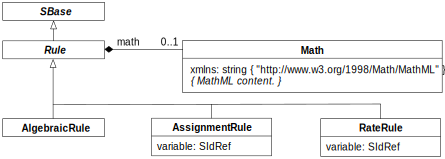
\includegraphics[scale=0.8]{figs/rule-uml}
  \caption{The definition of \RuleUpright and derived types
      \AlgebraicRule, \AssignmentRule and \RateRule.}
  \label{fig:rules}
\end{figure}



\subsubsection{Common attributes in \abstractclass{Rule}}
\label{sec:rule-math}\label{sec:rule-fields}\label{sec:rule-sboterm}

The classes derived from \Rule inherit \token{math} and the attributes and elements \changed{that \Rule itself inherits from \SBase, including \token{sboTerm} and \token{id}}.


\begin{blockChanged}
\paragraph{The \token{id} attribute}
\label{sec:rule-id}

\Rule inherits an optional \token{id} attribute from \SBase, of type \primtype{SId}.  The identifier of a \Rule-derived object has no mathematical meaning in a model.

\end{blockChanged}


\paragraphChanged{The \token{math} element}

A \Rule object has \changed{an optional} element called \token{math},
containing a MathML expression defining the mathematical formula
of the rule.  This MathML formula must return a numerical value.
The formula can be an arbitrary expression referencing the
variables and other entities in an SBML model.  The interpretation
of \token{math} and its associated unit of measurement are
described in more detail in Sections~\ref{sec:algebraicrule},
\ref{sec:assignmentrule} and~\ref{sec:raterule} below.


\paragraphChanged{The \token{sboTerm} attribute}

\Rule inherits an optional \token{sboTerm}
attribute of type \primtype{SBOTerm} from its parent
class \SBase (see Sections~\ref{sec:sboterm-type}
and~\ref{sec:sboTerm}).  When a value is given to this
attribute in an \AlgebraicRule, \AssignmentRule, or
\RateRule instance, it should be an
SBO identifier belonging to the branch for type  \AlgebraicRule, \AssignmentRule, or
\RateRule indicated in Table~\ref{tab:sboterm-availability}.  The relationship is
of the form ``the rule \emph{is-a} X'', where X is
the SBO term.  The term chosen should be the most precise (narrow)
one that captures the role of the rule in the model.

As discussed in Section~\ref{sec:sboTerm}, SBO labels are optional
information on a model.  Applications are free to ignore
\token{sboTerm} values.  A model must be interpretable without the
benefit of SBO labels.


\subsubsection{\class{AlgebraicRule}}
\label{sec:algebraicrule}

The rule type \AlgebraicRule is used to express equations that are
neither assignments of model variables nor rates of change.  The
\AlgebraicRule class does not add any attributes to the basic
\Rule; its role is simply to distinguish this case from the other
cases.  An example of the use of \AlgebraicRule is given in
Section~\ref{sec:algeraiceg}.

In the context of a simulation, algebraic rules are in effect at
all times, $t \geq 0$.  To allow evaluating expressions that
involve the \emph{delay} \token{csymbol}
(Section~\ref{sec:csymbol-token}), algebraic rules are considered
to apply also at $t \leq 0$.  Section~\ref{sec:before-t0}
describes the semantics of assignments, rules, and entity values
for simulation time $t \leq 0$.

An SBML model must not be overdetermined.  The ability to define
arbitrary algebraic expressions in an SBML model introduces the
possibility that a model is mathematically overdetermined by the
overall system of equations constructed from its rules, reactions
and events.  Therefore, if an algebraic rule is introduced in a
model, for at least one of the entities referenced in the rule's
\token{math} element the value of that entity must not be
completely determined by other constructs in the model.  This
means that at least this entity must not have the attribute
\token{constant}=\val{true} and there must also not be a rate rule
or assignment rule for it.  Furthermore, if the entity is a
\Species object, its value must not be determined by reactions,
which means that it must either have the attribute
\token{boundaryCondition}=\val{true} or else not be involved in
any reaction at all.  These restrictions are explained in more
detail in Section~\ref{sec:ruleconstraints} below.

Reaction identifiers can be referenced in the \token{math} 
expression of an algebraic rule, but reaction rates can never be
\emph{determined} by algebraic rules.  This is true even when a
reaction does not contain a \KineticLaw element.  (In such cases
of missing \KineticLaw elements, the model is valid but 
incomplete; the rates of reactions lacking kinetic laws are
simply undefined, and not determined by the algebraic rule.)


\subsubsection{\class{AssignmentRule}}
\label{sec:assignmentrule}

The rule type \AssignmentRule is used to express equations that
set the values of variables.  The left-hand side (the \changed{required}
\token{variable} attribute) of an assignment rule \changed{is of type \primtype{SIdRef}, and can refer to any SBML object in the \primtype{SId} namespace with mathematical meaning and the ability to be assigned.  In SBML Level~3 Core, this consists of}
\Species, \SpeciesReference, \Compartment, 
\changed{and} global \Parameter objects in
the model (but not reactions).  The entity identified must
%NB:  changed to make this text match that for RateRule:
\changed{have its \token{constant} attribute set to the value \val{false}}.  The effects of
an \AssignmentRule are in general terms the same, but differ in
the precise details depending on the type of variable being set:

\begin{itemize}
  
\item \emph{In the case of a species}, an \AssignmentRule sets the
  referenced species' quantity (whether a \quantity{concentration}
  or \quantity{amount}) to the value determined by the formula in
  \token{math}.  The unit associated with the value produced by
  the \token{math} formula should be equal to the unit associated
  with the species' quantity.  (See
  Section~\ref{sec:species-units} for an explanation of how a
  species' quantity is determined.)
  
  \emph{Restrictions}: There must not be both an \AssignmentRule
  \token{variable} attribute and a \SpeciesReference \token{species}
  attribute having the same value, unless that species has its
  \token{boundaryCondition} attribute set to \val{true}.  In other
  words, an assignment rule cannot be defined for a species that
  is created or destroyed in a reaction unless that species is
  defined as a boundary condition in the model.

\item \emph{In the case of a species reference}, an
  \AssignmentRule sets the stoichiometry of the corresponding
  reactant or product to the value determined by the formula in
  \token{math}.  The unit associated with the value produced by
  the \token{math} formula should be consistent with the unit
  \token{dimensionless}, because reactant and product
  stoichiometries in reactions are dimensionless quantities.

\item \emph{In the case of a compartment}, an \AssignmentRule sets
  the referenced compartment's size to the size determined by the
  formula in \token{math}.  The unit associated with the value
  produced by the \token{math} formula should be the same as that
  specified for the compartment's size.  (See
  Section~\ref{sec:compartment-units} for more information about
  compartment units.)
  
\item \emph{In the case of a parameter}, an \AssignmentRule sets
  the referenced parameter's value to the value of the formula in
  \token{math}.  The unit associated with the value produced by
  the formula should be the same as parameter's \token{units}
  attribute value.  (See Section~\ref{sec:parameter-units} for
  more information about parameter units.)

\begin{blockChanged}
\item \emph{In the case of an object from an SBML Level~3 package}, an \AssignmentRule sets
  the referenced object's value (as defined by that package) to the value of the formula in
  \token{math}.  The unit of measurement associated with the value produced by
  the formula should be the same as that object's \token{units}
  attribute value (if it has such an attribute), or be equal to
  the units of model components of that type (if objects of that class
  are defined by the package as having the same units).
\end{blockChanged}

\end{itemize}


\begin{blockChanged}

If the \token{variable} attribute of an \AssignmentRule object references an object in an SBML namespace that is not understood by the interpreter reading a given SBML document (that is, if the object is defined by an SBML Level~3 package that the software does not support), the assignment rule must be ignored---the object's value will not need to be set, as the interpreter could not understand that package.  If an interpreter cannot establish whether a referenced object is missing from the model or instead is defined in an SBML namespace not understood by the interpreter, it may produce a warning to the user.  (The latter situation may only arise if an SBML package is present in the SBML document with a \token{package:required} attribute of \val{true}.)

\end{blockChanged}

In the context of a simulation, assignment rules are in effect at
all times, $t \geq 0$.  For purposes of evaluating expressions
that involve the \emph{delay} \token{csymbol}
(Section~\ref{sec:csymbol-token}), assignment rules are considered
to apply also at $t \leq 0$.  Section~\ref{sec:before-t0} provides
additional information about how $t \leq 0$ should be
  handled.

A model must not contain more than one \AssignmentRule or
\RateRule object having the same value of \token{variable}; in
other words, in the set of all assignment rules and rate rules in
an SBML model, each variable appearing in the left-hand sides can
only appear once.  This simply follows from the fact that an
indeterminate system would result if a model contained more than
one assignment rule for the same variable or both an assignment
rule and a rate rule for the same variable.

Similarly, a model must also not contain \emph{both} an
\AssignmentRule and an \InitialAssignment for the same variable,
because both kinds of constructs apply prior to and at the start
of simulation time, \ie $t \leq 0$.  If a model contained both an
initial assignment and an assignment rule for the same variable,
an indeterminate system would result.  (See also
Section~\ref{sec:initial-assignment-semantics}.)

The value calculated by an \AssignmentRule object overrides the
value assigned to the given symbol by the object defining that
symbol.  For example, if a \Compartment's \token{size} is set in
its definition, and the model also contains an \AssignmentRule
having that compartment's \token{id} as its \token{variable}
value, then the \token{size} assigned in the \Compartment
definition is ignored and the value assigned based on the
computation defined in the \AssignmentRule.  This does \emph{not}
mean that a definition for a given symbol can be omitted if there
is an \AssignmentRule object for it.  For example, there must be a
\Parameter definition for a given parameter if there is an
\AssignmentRule for that parameter.


\subsubsection{\class{RateRule}}
\label{sec:raterule}

The rule type \RateRule is used to express equations that
determine the rates of change of variables.  The left-hand side
(the \changed{required} \token{variable} attribute) of a rate rule  \changed{is of type \primtype{SIdRef}, and can refer to any SBML object in the \primtype{SId} namespace with mathematical meaning and the ability to be assigned.  In SBML Level~3 Core, this consists of}
\Species, \SpeciesReference, \Compartment, 
\changed{and} global \Parameter objects in
the model (but not reactions).  The
entity identified must have its \token{constant} attribute set to
\val{false}.  The effects of a \RateRule are in general terms the
same, but differ in the precise details depending on which
variable is being set:

\begin{itemize}
  
\item \emph{In the case of a species}, a \RateRule sets the rate
  of change of the species' quantity (\quantity{concentration} or
  \quantity{amount}) to the value determined by the formula in
  \token{math}.  The unit associated with the rule's \token{math}
  element should be equal to the unit of the species' quantity
  (Section~\ref{sec:species-units}) divided by the model-wide unit
  of \quantity{time} (Section~\ref{sec:timeunits}), or in other
  words, \{unit of \quantity{species quantity}\}/\{unit of
  \quantity{time}\}.

  \emph{Restrictions}: There must not be both a \RateRule
  \token{variable} attribute and a \SpeciesReference \token{species}
  attribute having the same value, unless that species has its
  \token{boundaryCondition} attribute is set to \val{true}.  This
  means a rate rule cannot be defined for a species that is
  created or destroyed in a reaction, unless that species is
  defined as a boundary condition in the model.

\item \emph{In the case of a species reference}, a \RateRule sets
  the rate of change of the stoichiometry of the referenced
  reactant or product to the value determined by the formula in
  \token{math}.  The unit associated with the value produced by
  the formula should be consistent with \{unit derived from
  \token{dimensionless}\}/\{unit of \quantity{time}\}.
  
\item \emph{In the case of a compartment}, a \RateRule sets the
  rate of change of the compartment's size to the value determined
  by the formula in \token{math}.  The unit of the rule's
  \token{math} element should be identical to the compartment's
  \token{units} attribute divided by the model-wide unit of
  \quantity{time}.  (In other words, \{unit of
  \quantity{compartment size}\}/\{unit of \quantity{time}\}.)

\item \emph{In the case of a parameter}, a \RateRule sets the rate
  of change of the parameter's value to that determined by the
  formula in \token{math}.  The unit associated with the rule's
  \token{math} element should be equal to the parameter's
  \token{units} attribute value divided by the model-wide unit of
  \quantity{time}.  (In other words, \{parameter
  \token{units}\}/\{unit of \quantity{time}\}.)

\begin{blockChanged}
\item \emph{In the case of an object from an SBML Level~3 package}, a \RateRule sets the rate of change of the referenced object's value (as defined by that package) to the value of the formula in \token{math}.    The unit of measurement associated with the value produced by
  the formula should be the same as that object's \token{units}
  attribute value (if it has such an attribute), or be equal to
  the units of model components of that type (if objects of that class
  are defined by the package as having the same units).
\end{blockChanged}

\end{itemize}

\begin{blockChanged}

If the \token{variable} attribute of an \AssignmentRule object references an object in an SBML namespace that is not understood by the interpreter reading a given SBML document (that is, if the object is defined by an SBML Level~3 package that the software does not support), the rate rule must be ignored---the object's value will not need to be set, as the interpreter could not understand that package.  If an interpreter cannot establish whether a referenced object is missing from the model or instead is defined in an SBML namespace not understood by the interpreter, it may produce a warning to the user.  (The latter situation may only arise if an SBML package is present in the SBML document with a \token{package:required} attribute of \val{true}.)

\end{blockChanged}

In the context of a simulation, rate rules are in effect for
simulation time $t > 0$.  Other types of rules and initial
assignments are in effect at different times;
Section~\ref{sec:before-t0} describes these conditions.

As mentioned in Section~\ref{sec:assignmentrule} for
\AssignmentRule, a model must not contain more than one \RateRule
or \AssignmentRule object having the same value of
\token{variable}; in other words, in the set of all assignment
rules and rate rules in an SBML model, each variable appearing in
the left-hand sides can only appear once.  This simply follows
from the fact that an indeterminate system would result if a model
contained more than one assignment rule for the same variable or
both an assignment rule and a rate rule for the same variable.


\subsubsection{Additional restrictions on rules}
\label{sec:ruleconstraints}

An important design goal of SBML rule semantics is to ensure that
a model's simulation and analysis results will not be dependent on
when or how often rules are evaluated.  To achieve this, SBML
needs to place two additional restrictions on rule use in addition
to the conditions described above regarding the use of
\AlgebraicRule, \AssignmentRule and \RateRule.  The first concerns
algebraic loops in the system of assignments in a model, and the
second concerns overdetermined systems.


\paragraph{The model must not contain algebraic loops}

The combined set of \InitialAssignment, \AssignmentRule and
\KineticLaw objects constitute a set of assignment statements that
should be considered as a whole.  (A \KineticLaw object is counted
as an assignment because it assigns a value to the symbol
contained in the \token{id} attribute of the \Reaction object in which
it is defined.)  This combined set of assignment statements must
not contain algebraic loops---dependency chains between these
statements must terminate.  To put this more formally, consider a
directed graph in which nodes are assignment statements and
directed arcs exist for each occurrence of an SBML species, species reference,
compartment or parameter symbol in an assignment statement's
\token{math} element.  Let the directed arcs point from the
statement assigning the symbol to the statements that contain the
symbol in their \token{math} element expressions.  This graph must
be acyclic.

\begin{blockChanged}

Similarly, the combined set of \RateRule and \Reaction objects constitute a set of definitions for the rates of change of various model entities (namely, the objects identified by the values of the \token{variable} attributes of the \RateRule objects, and the \token{species} attributes of the \SpeciesReference objects in each \Reaction).  These rates of change may be referenced directly using the \emph{rateOf} \token{csymbol}, but may not thereby contain algebraic loops---dependency chains between these statements must terminate.  More formally, consider a directed graph in which the nodes are the definitions of different variables' rates of change, and directed arcs exist for each occurrence of a variable referenced by a \emph{rateOf} \token{csymbol} from any \RateRule or \KineticLaw object in the model.  Let the directed arcs point from the variable referenced by the \emph{rateOf} \token{csymbol} (call it \emph{x}) to the variable(s) determined by the \token{math} expression in which \emph{x} appears.  This graph must be acyclic.

\end{blockChanged}

SBML does not specify when or how often rules should be evaluated.
Eliminating algebraic loops ensures that assignment statements can
be evaluated any number of times without the result of those
evaluations changing.  As an example, consider the following
equations:
\begin{linenomath}
\begin{equation*}
  \begin{array}{lll}
    x = x + 1, & y = z + 200, & z = y + 100
  \end{array}
\end{equation*}
\end{linenomath}
If this set of equations were interpreted as a set of assignment
statements, it would be invalid because the rule for $x$ refers to
$x$ (exhibiting one type of loop), and the rule for $y$ refers to
$z$ while the rule for $z$ refers back to $y$ (exhibiting another
type of loop).

Conversely, the following set of equations would constitute a
valid set of assignment statements:
\begin{linenomath}
\begin{equation*}
  \begin{array}{lll}
    x = 10, & y = z + 200, & z = x + 100
  \end{array}
\end{equation*}
\end{linenomath}


\paragraph{The model must not be overdetermined}

An SBML model must not be overdetermined; that is, a model must
not define more equations than there are unknowns in a model.  An
SBML model without \AlgebraicRule objects cannot be
overdetermined.

Assessing whether a given continuous, deterministic, mathematical
model is overdetermined does not require dynamic analysis; it can
be done by analyzing the system of equations created from the
model.  It should be noted that when a model contains both
reactions and events, there are several sets of equations to
consider in order to assess whether a model is overdetermined.
The set of equations derived from the combined set of rules and
reactions and, for each event, the set of equations derived from
the combined set of rules and event assignments for the particular
event.

One approach is to construct a bipartite graph in which one set of
vertices represents the variables and the other set of vertices
represents the equations.  The approach involves placing edges
between vertices such that variables in the system are linked to
the equations that determine them.  A mathematical model is
overdetermined if the maximal matchings~\citep{chartrand_1977} of
the bipartite graph contain disconnected vertexes representing
equations.  (If one maximal matching has this property, then all
the maximal matchings will have this property; \ie it is only
necessary to find one maximal matching.)
Appendix~\ref{apdx:assessing-overdetermined} describes a method of
applying this procedure to specific SBML data objects.  In some
cases it is possible to avoid the use of an \AlgebraicRule.  This
is discussed in more detail in Section~\ref{sec:bp:rules}.


\subsubsection{Example of rule use}
\label{sec:eg-rule-use}

This section contains an example set of rules.  Consider the
following set of equations:
\begin{linenomath}
  \begin{equation*}
    \begin{array}{lll}
      k = \dfrac{k_3}{k_2}, & s_2 = \dfrac{k \cdot x}{1 + k_2}, & A = 0.10 \cdot x
    \end{array}
  \end{equation*}
\end{linenomath}
This can be encoded by the following scalar rule set (where the
definitions of \texttt{x}, \texttt{s}, \texttt{k}, \texttt{k2},
\texttt{k3} and \texttt{A} are assumed to be located elsewhere in
the model and not shown in this abbreviated example):

\begin{example}
<listOfRules>
    <assignmentRule variable="k">
        <math xmlns="http://www.w3.org/1998/Math/MathML">
            <apply> <divide/> <ci> k3 </ci> <ci> k2 </ci> </apply>
        </math>
    </assignmentRule>
    <assignmentRule variable="s2">
        <math xmlns="http://www.w3.org/1998/Math/MathML">
            <apply>
                <divide/>
                    <apply> <times/> <ci> k </ci> <ci> x </ci> </apply>
                    <apply> <plus/> <cn> 1 </cn> <ci> k2 </ci> </apply>
            </apply>
        </math>
    </assignmentRule>
    <assignmentRule variable="A">
        <math xmlns="http://www.w3.org/1998/Math/MathML">
            <apply> <times/> <cn> 0.10 </cn> <ci> x </ci> </apply>
        </math>
    </assignmentRule>
</listOfRules>
\end{example}


%-----------------------------------------------------------------------------
\subsection{Constraints}
\label{sec:constraints}
%-----------------------------------------------------------------------------

The \Constraint object is a mechanism for stating the
assumptions under which a model is designed to operate.  The
\emph{constraints} are statements about permissible values of
different quantities in a model.  Figure~\ref{fig:constraint}
shows the definition of the \Constraint object class.

\begin{figure}[htb]
  \centering
  \small
  \vspace*{2ex}
  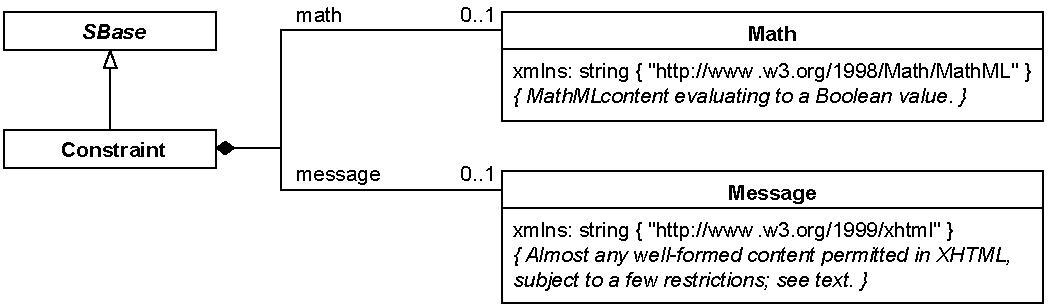
\includegraphics[scale=0.8]{figs/constraint-uml}
  \caption{The definition of class \Constraint.  The contents of
    the \Math class can be any \mathml permitted in SBML,
    but it must return a boolean value.  As shown above, an
    instance of \Constraint can also contain zero or one instances
    of \Message objects; this class of object is simply a wrapper
    (in the XML form, \token{<message> \ldots{} </message>}) for
    XHTML content.  The same guidelines for XHTML content as
    explained in Section~\ref{sec:notes} for notes on \SBaseUpright also
    apply to the XHTML within messages in a \Constraint. A
    sequence of \changed{zero} or more instances of \Constraint objects can
    be located in an instance of \ListOfConstraints in \Model, as
    shown in Figure~\protect\ref{fig:model}.}
  \label{fig:constraint}
\end{figure}

The essential meaning of a constraint is this: if a dynamical
analysis of a model (such as a simulation) reaches a state in
which a constraint is no longer satisfied, the results of the
analysis are deemed invalid beginning with that point in time.
The exact behavior of a software tool, upon encountering a
constraint violation, is left up to the software; \emph{however},
a software tool must somehow indicate to the user when a model's
constraints are no longer satisfied.  (Otherwise, a user may not
realize that the analysis has reached an invalid state and is
potentially producing nonsense results.)  If a software tool does
not have support for constraints, it should indicate this to the
user when encountering a model containing constraints.


\begin{blockChanged}
\paragraph{The \token{id} attribute}
\label{sec:constraint-id}

\Constraint inherits an optional \token{id} attribute from \SBase, of type \primtype{SId}.  The identifier of a \Constraint object has no mathematical meaning in an SBML \thisLV model.

\end{blockChanged}


\paragraphChanged{The \token{sboTerm} attribute}
\label{sec:constraint-sboterm}

\Constraint inherits an optional \token{sboTerm}
attribute of type \primtype{SBOTerm} from its parent
class \SBase (see Sections~\ref{sec:sboterm-type}
and~\ref{sec:sboTerm}).  When a value is given to this
attribute in a  \Constraint instance, it should be an
SBO identifier belonging to the branch for type  \Constraint
indicated in Table~\ref{tab:sboterm-availability}.  The relationship is
of the form ``the constraint \emph{is-a} X'', where X is
the SBO term.  The term chosen should be the most precise (narrow)
one that captures the role of the constraint in the model.

As discussed in Section~\ref{sec:sboTerm}, SBO labels are optional
information on a model.  Applications are free to ignore
\token{sboTerm} values.  A model must be interpretable without the
benefit of SBO labels.


\subsubsection{The \token{math} element}

\Constraint has one \changed{optional} subelement, \token{math},
containing a MathML formula defining the condition of the
constraint.  This formula must return a boolean value of
\val{true} when the model is in a \emph{valid} state.  The formula
can be an arbitrary expression referencing the variables and other
entities in an SBML model.  The evaluation of \token{math} and
behavior of constraints are described in more detail in
Section~\ref{sec:constraint-semantics} below.


\subsubsection{\class{Message}}
\label{sec:constraint-message}

A \Constraint object can contain an optional element named
\token{message} whose content is determined by object class \Message.
This element can contain a message in XHTML format that may be
displayed to the user when the condition of the constraint in
\token{math} evaluates to a value of \val{false}.  Software tools
are not required to display the message, but it is recommended
that they do so as a matter of best practice.

The XHTML content within a \Message object must follow the same
restrictions as for \Notes objects described in
Section~\ref{sec:notes}.  In particular, the element must declare
the use of the XHTML XML namespace, and must not contain an XML
declaration or a DOCTYPE declaration.


\subsubsection{Semantics of constraints}
\label{sec:constraint-semantics}

In the context of a simulation, a \Constraint has effect at all
times $t \geq 0$.  Each \Constraint's \token{math} element is first
evaluated after any \InitialAssignment definitions in a model at
$t = 0$ and can conceivably trigger at that point.  (In other
words, a simulation could fail a constraint immediately.)

\Constraint definitions \emph{cannot and should not} be used to
compute the dynamical behavior of a model as part of, for example,
simulation.  \changed{Constraints may be used as input to non-dynamical
analysis.}

The results of a simulation of a model containing a constraint are
invalid from any simulation time at and after a point when the
function given by the \token{math} returns a value of \val{false}.
Invalid simulation results do not make a prediction of the
behavior of the biochemical reaction network represented by the
model.  The precise behavior of simulation tools is left undefined
with respect to constraints.  If invalid results are detected with
respect to a given constraint, the contents of the \Message
subobject (Section~\ref{sec:constraint-message}) may optionally be
displayed to the user.  The simulation tool may also halt the
simulation or clearly delimit in output data the simulation time
point at which the simulation results become invalid.

There are no restrictions on duplicate \Constraint
definitions or the order of evaluation of \Constraint objects in a
model.  It is possible for a model to define multiple constraints
all with the same \token{math} element.  Since the failure of any
constraint indicates the simulation has entered an invalid state,
a system is not required to attempt detecting whether
other constraints in the model have failed once any one constraint
has failed.


\subsubsection{Example}

As an example, the following SBML fragment demonstrates the
constraint that species \val{S1} should only have values between~1
and~100:

\begin{example}
<model ...>
    ...
    <listOfConstraints>
        <constraint>
            <math xmlns="http://www.w3.org/1998/Math/MathML"
                  xmlns:sbml="http://www.sbml.org/sbml/level3/version2/core">
                <apply>
                    <and/>
                        <apply> 
                          <lt/> 
                          <cn sbml:units="mole"> 1 </cn> 
                          <ci> S1 </ci> 
                        </apply>
                        <apply> 
                          <lt/> 
                          <ci> S1 </ci>  
                          <cn sbml:units="mole"> 100 </cn> 
                        </apply>
                </apply>
            </math>
            <message>
                <p xmlns="http://www.w3.org/1999/xhtml"> Species S1 is out of range. </p>
            </message>
        </constraint>
    </listOfConstraints>
    ...
</model>
\end{example}


%-----------------------------------------------------------------------------
\subsection{Reactions}
\label{sec:reactions}
%-----------------------------------------------------------------------------

A \emph{reaction} in SBML represents any kind of process that can
change the quantity of one or more species in a model.  Examples
of such processes can include transformation, transport, molecular
interactions, and more.  In SBML, the notion of a reaction is
generalized to allow entities that may not be chemical substances;
thus, a reaction in SBML does not necessarily have to be a
biochemical reaction---a biochemical reaction is just one possible
kind of process.

At minimum, to describe a reaction in SBML, it is necessary to
define its \emph{structural} properties, specifically the
participating reactants and/or products (and their corresponding
stoichiometries) and the reversibility of the process.  In
addition, an SBML reaction can also contain a \emph{quantitative}
description of the rate of the reaction; this aspect consists of a
mathematical formula expressing describing the rate at which the
reaction process takes place, together with an optional list of
modifier species and parameters influencing the reaction rate.
The various parts of a reaction are recorded in the SBML \Reaction
object class and other supporting data classes, defined in
Figure~\vref{fig:reaction}.

\begin{figure}[b]
  \centering
  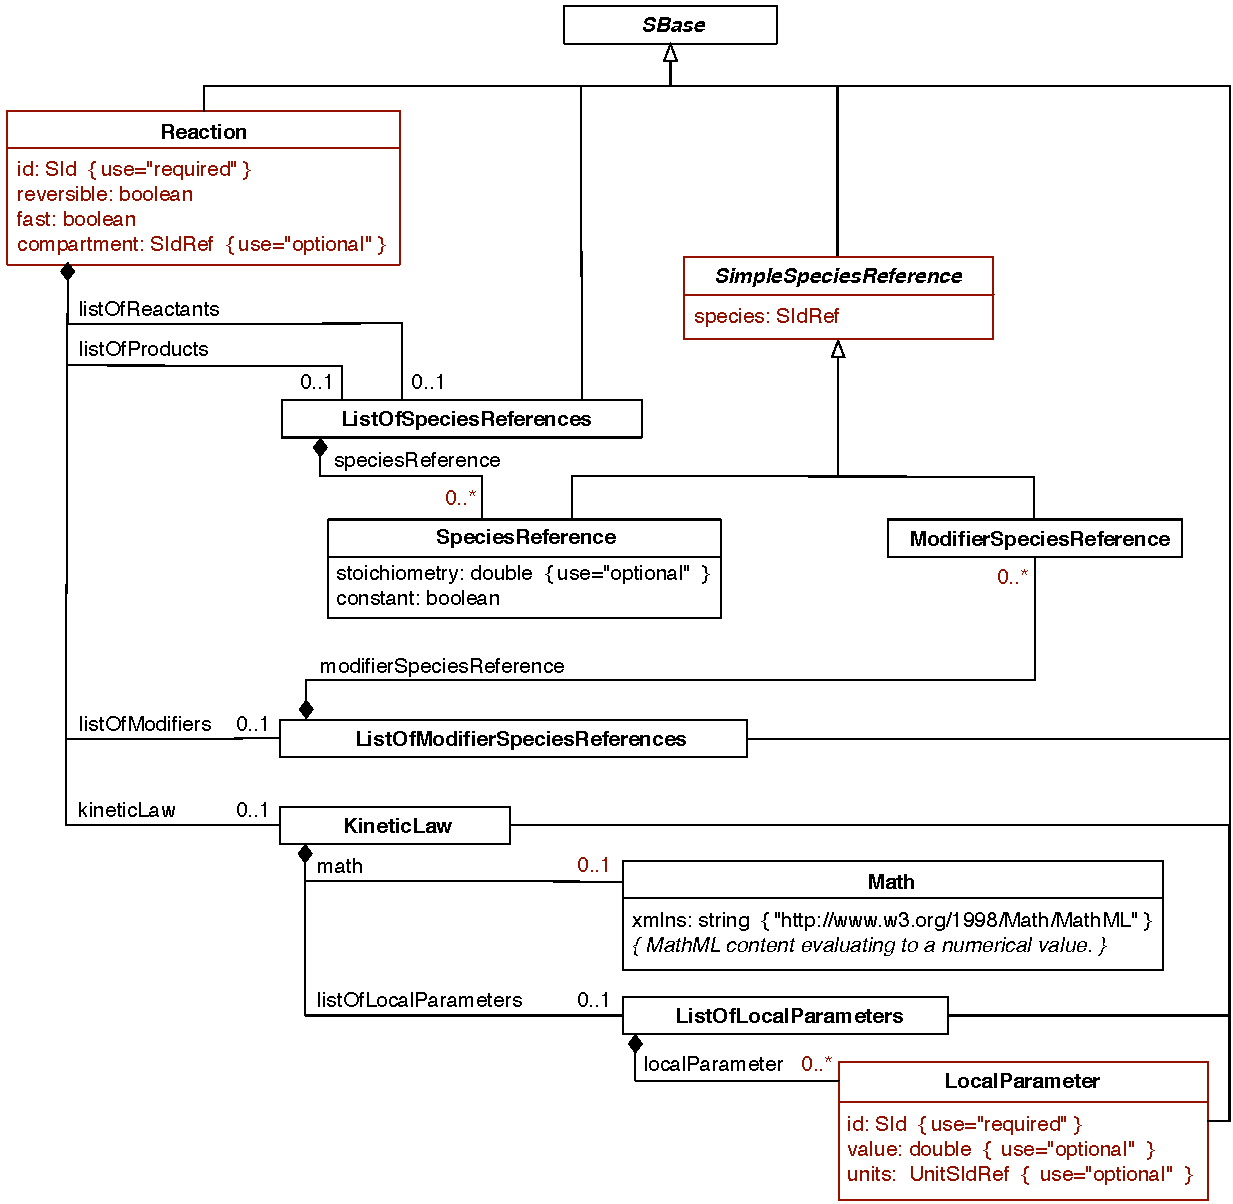
\includegraphics[scale=0.78]{figs/reaction-uml-v2}
  \caption{The definitions of \Reaction, \KineticLaw,
    \SpeciesReference, \ModifierSpeciesReference, \LocalParameter,
    as well as the container classes \ListOfSpeciesReferences,
    \ListOfModifierSpeciesReferences, and \ListOfLocalParameters.
    Note that \SimpleSpeciesReferenceUpright is an abstract class used
    only to provide some common attributes to its derived
    classes.}
  \label{fig:reaction}
\end{figure}


\subsubsection{\class{Reaction}}
\label{sec:reaction-type}
\label{sec:listofreactants}
\label{sec:listofproducts}
\label{sec:listofmodifiers}

Each reaction in an SBML model is defined using an instance of a
\Reaction object.  As shown in Figure~\vref{fig:reaction}, it
contains several scalar attributes and several lists of other
objects.


\begin{blockChanged}
\paragraph{The \token{id} attribute}

Like other classes in SBML \thisLV, \Reaction inherits the \token{id} attribute from \SBase; however, \Reaction defines \token{id} as being required rather than optional.  The attribute otherwise behaves as described in Section~\ref{sec:idnameattribs}.

The identifier (the \token{id} attribute value) of a \Reaction object may be used in a model's mathematical expressions.  The identifier stands for the reactions rate; this is explained in more detail in Section~\ref{subsec:reaction-as-symbol}.  A reaction's identifier cannot be the target of an \InitialAssignment, \EventAssignment, or \Rule object, nor may its value be determined by an \AlgebraicRule object in a model.

\end{blockChanged}


\paragraph{The lists of reactants, products and modifiers}

Each species participating as a reactant, product, and/or modifier
in a reaction must be declared using a \SpeciesReference and/or
\ModifierSpeciesReference object stored in the list elements
\token{listOfReactants}, \token{listOfProducts} and
\token{listOfModifiers}.  The object classes \SpeciesReference and
\ModifierSpeciesReference are described in more detail in
Sections~\ref{subsec:speciesreference}
and~\ref{subsec:modifierreference} below.  Throughout this text,
we use the informal expressions ``list of reactants'', ``list of
products'' and ``list of modifiers'' to mean, respectively, the
list of species identified by \SpeciesReference objects within a
\Reaction \token{listOfReactants} element, the list of species
identified by \SpeciesReference objects within a \Reaction
\token{listOfProducts} element, and the list of species identified
by \ModifierSpeciesReference objects within a \Reaction
\token{listOfModifiers} element.

Certain restrictions are placed on the appearance of species in
reaction definitions:
\begin{itemize}
  
\item The ability of a species to appear as a reactant or product
  of any reaction in a model is governed by certain combinations
  of the attributes \token{constant} and \token{boundaryCondition}
  on the \Species object instance; see
  Section~\ref{sec:species-constant} for more information.
  
\item Any species appearing in the \token{math} element of the
  \token{kineticLaw} of a \Reaction instance must be declared in
  at least one of that \Reaction's lists of reactants, products,
  and/or modifiers.  It is an error for a reaction's kinetic law
  formula to refer to species that have not been declared for that
  reaction.
  
\item A reaction definition can contain an empty list of reactants
  \emph{or} an empty list of products, but it must have at least
  one reactant or product; in other words, a reaction without any
  reactant or product species is not permitted.  (This restriction
  does not apply to modifier species, which are always optional.)

\end{itemize}


\paragraph{The \token{kineticLaw} element}

A \Reaction object can contain up to one \KineticLaw object, in
the \token{kineticLaw} element.  This ``kinetic law'' defines the
speed at which the process defined by the reaction takes place.  A
more detailed description of \KineticLaw is left to
Section~\ref{subsec:kinetic-law} below.

The inclusion of a \KineticLaw object in an instance of a
\Reaction is optional.  For some modeling purposes, models
containing reactions without defined rates are an acceptable
alternative (and may even be the only possible option, such as
when the kinetics of the reactions are unknown).  However, missing
kinetic laws preclude the application of many model analysis
techniques, including simulation.


\paragraph{The \token{reversible} attribute}
\label{sec:reversible}

The mandatory boolean attribute \token{reversible} on \Reaction
indicates whether the reaction is reversible.  To say that a
reaction is \emph{reversible} is to say it can proceed in either
the forward or the reverse direction.  This information may be
redundant in cases where the reversibility of the reaction can be
deduced by inspecting the rate formula given in the kinetic law.
However, a reaction is not required to have a kinetic law, and
besides, when a rate expression is present, it may not always be
possible to deduce the reversibility by inspecting it.  Having a
separate attribute for \token{reversible} allows certain kinds of
structural analysis, such as elementary mode analysis, even in
these cases.

Mathematically, the \token{reversible} attribute on \Reaction has
no impact on the construction of the equations for change of the
species quantities.  However, labeling a reaction as irreversible
is interpreted as an assertion that the rate expression will not
have negative values during a simulation.  Software developers may
wish to provide their software systems with a means of testing
that this condition holds.

The presence of reversibility information in two places (\ie the
rate expression in the kinetic law, and the \token{reversible}
flag) leaves open the possibility that a model could contain
contradictory information, but this would be considered to be an
error of the encoded model, rather than an invalid SBML encoding.


\paragraph{The \token{fast} attribute}
\label{sec:fast}

The boolean attribute \token{fast} is another required boolean
attribute of \Reaction.  When a model contains a value of
\val{true} for \token{fast} on any of its reactions, it indicates
that the creator of the model is distinguishing different time
scales of reactions in the system.  If a model does not
distinguish between time scales, the \token{fast} attribute should
be set to \val{false} for all reactions.

The model's reactions are divided into two sets by the
values of the \token{fast} attributes.  The set of reactions
having \token{fast}=\val{true} (known as \emph{fast reactions})
should be assumed to be operating on a time scale significantly
faster than the other reactions (the \emph{slow reactions}).  Fast
reactions are considered to be instantaneous relative to the slow
reactions.  Software tools should use a pseudo steady-state
approximation for the set of fast reactions when constructing the
system of equations for the model.  More specifically, the set of
reactions that have the \token{fast} attribute set to \val{true}
forms a subsystem that should be described by a pseudo
steady-state approximation in relationship to all other reactions
in the model.  Under this description, relaxation from any initial
condition or perturbation from any intermediate state of this
subsystem would be infinitely fast.
Appendix~\ref{apdx:consequences-of-being-fast} provides a
technical explanation of an approach to solving systems with fast
reactions.

The correctness of the approximation requires a significant
separation of time scales between the fast reactions and other
processes.  It is the responsibility of the modeler or of the
software system writing the SBML model to ensure this condition is
fulfilled.

Note that the \token{fast} attribute has a significant effect on
the mathematical interpretation of a model and cannot be safely
ignored if a software tool does not implement support for the
corresponding concept.  Software systems should indicate to users
when they encounter models with reactions having
\token{fast}=\val{true} and do not have the capacity to analyze
the model using a pseudo steady-state approximation.

\begin{blockChanged}
In SBML Level~3 Version~2, the \token{fast} attribute is deprecated.  The attribute will be removed in future versions of SBML, and the speed of every \Reaction will be always be determined by its \KineticLaw.  Beginning in SBML Level~3 Version~2, it is best practice to always produce models with a \token{fast} attribute value of \val{false}.  To achieve the same or similar effects as setting the \token{fast} attribute to \val{true} for a given reaction, the \KineticLaw attribute should be constructed to produce a value in the desired time scale, or else the reaction could be replaced with an \AssignmentRule or \AlgebraicRule object as in the example of Section~\ref{apdx:rules-eg}.
\end{blockChanged}


\paragraph{The \token{compartment} attribute on \class{Reaction}}
\label{sec:reaction-compartment}

The optional attribute \token{compartment}, of data type
\primtype{SIdRef}, can be used to indicate the compartment in
which the reaction is assumed to take place.  If the attribute is
present, its value must be the identifier of a \Compartment object
defined in the enclosing \Model object.

Similar to the \token{reversible} attribute, the value of the
\token{compartment} attribute has no direct impact on the
construction of mathematical equations for the SBML model.  When a
reaction has a kinetic law, the compartment location may already
be implicit in the kinetic law (though this cannot always be
guaranteed).  Nevertheless, software tools may find the
\token{compartment} attribute value useful for such purposes as
analyzing the structure of the model, guiding the modeler in
constructing correct rate formulas, and visualization.


\paragraph{The \token{sboTerm} attribute on \class{Reaction}}
\label{sec:reaction-sboterm}

\Reaction inherits an optional \token{sboTerm}
attribute of type \primtype{SBOTerm} from its parent
class \SBase (see Sections~\ref{sec:sboterm-type}
and~\ref{sec:sboTerm}).  When a value is given to this
attribute in a  \Reaction instance, it should be an
SBO identifier belonging to the branch for type  \Reaction  
indicated in Table~\ref{tab:sboterm-availability}.  The relationship is
of the form ``the reaction \emph{is-a} X'', where X is
the SBO term.  The term chosen should be the most precise (narrow)
one that captures the role of the reaction in the model.

As discussed in Section~\ref{sec:sboTerm}, SBO labels are optional
information on a model.  Applications are free to ignore
\token{sboTerm} values.  A model must be interpretable without the
benefit of SBO labels.


\subsubsection{\class{SimpleSpeciesReference}}
\label{subsec:simplespeciesreference}

As mentioned above, every species that enters into a given
reaction must appear in that reaction's lists of reactants,
products and/or modifiers.  In an SBML model, all species that may
participate in any reaction are listed in the \ListOfSpecies
object of the top-level \Model object instance (see
Section~\ref{sec:model}).  The lists of products, reactants and
modifiers in \Reaction objects do not introduce new species, but
rather, they refer back to those listed in the model's top-level
\ListOfSpecies object.  For reactants and products, the connection
is made using a \SpeciesReference object; for modifiers, it is
made using a \ModifierSpeciesReference object.
\SimpleSpeciesReference, defined in Figure~\vref{fig:reaction}, is
an abstract type that serves as the parent class of both
\SpeciesReference and \ModifierSpeciesReference.  It is used
simply to hold the attributes and elements that are common to the
latter two objects.


\paragraph{The \token{species} attribute}

The \SimpleSpeciesReference object class has \changed{a required attribute,
\token{species}, of data type \primtype{SIdRef},
inherited by \SpeciesReference and
\ModifierSpeciesReference.}  The value of \token{species} must be
the identifier of a species defined in the enclosing \Model; the
referenced species is thereby declared as participating in the
reaction being defined.  The precise role of that species as a
reactant, product, or modifier in the reaction is determined by
the subtype of \SimpleSpeciesReference (\ie either
\SpeciesReference or \ModifierSpeciesReference) in which the
identifier appears and by the specific list of species references
in which the \SpeciesReference appears.


\paragraph{The \token{sboTerm} attribute}
\label{sec:simplespeciesreference-sboterm}

\SimpleSpeciesReference inherits an optional \token{sboTerm}
attribute of type \primtype{SBOTerm} from its parent class \SBase
(see Sections~\ref{sec:sboterm-type} and~\ref{sec:sboTerm}).  When
a value is given to this attribute in a \SimpleSpeciesReference
instance, it should be an SBO identifier belonging to the branch
for type \SimpleSpeciesReference indicated in
Table~\ref{tab:sboterm-availability}.  The relationship is of the
form ``the species reference \emph{is-a} X'', where X is the SBO
term.  The term chosen should be the most precise (narrow) one
that captures the role of the species reference in the model.

As discussed in Section~\ref{sec:sboTerm}, SBO labels are optional
information on a model.  Applications are free to ignore
\token{sboTerm} values.  A model must be interpretable without the
benefit of SBO labels.


\subsubsection{\class{SpeciesReference}}
\label{subsec:speciesreference}

\Reaction provides a way to express which species act as reactants
and which species act as products in a reaction, and to declare
their stoichiometries.  This is done using \SpeciesReference
objects.  As mentioned above in
Section~\ref{subsec:simplespeciesreference}, \SpeciesReference
inherits the mandatory attribute \token{species} and optional
attributes \token{id}, \token{name}, and \token{sboTerm} from the
parent type \SimpleSpeciesReference.  It also defines the optional
attribute \token{stoichiometry} and the mandatory attribute
\token{constant}, described below.


\begin{blockChanged}
\paragraph{The \token{id} attribute}

The \token{id} attribute that \SpeciesReference inherits from \SBase is still optional, and behaves as described in Section~\ref{sec:idnameattribs}.  It also acquires the mathematical meaning of the value of its \token{stoichiometry} attribute, and may be the target of an \InitialAssignment, \EventAssignment, or \Rule object defined in the enclosing model.
\end{blockChanged}

\paragraph{The \token{stoichiometry} attribute}

The {\em stoichiometry} of a species in a reaction describes how
much of the species changes when a reaction event takes place.  In
SBML, product and reactant stoichiometries are specified using the
optional \token{stoichiometry} on \SpeciesReference object.  \changed{The
\token{stoichiometry} attribute is of type \primtype{double}.}  A missing
\token{stoichiometry} implies that the stoichiometry is either
unknown, or to be obtained from an external source, or determined
by an initial assignment (Section~\ref{sec:initialAssignment}) or
other SBML construct elsewhere in the model.

A species reference's stoichiometry is set by its
\token{stoichiometry} attribute exactly once.  If the
\SpeciesReference object's \token{constant} attribute (see below)
has the value \val{true}, then the stoichiometry is fixed and
cannot be changed except by an \InitialAssignment.  These two
methods of setting the stoichiometry (\ie using
\token{stoichiometry} directly, or using an \InitialAssignment)
differ in that the \token{stoichiometry} attribute can only be set
to a literal floating-point number, whereas \InitialAssignment
allows the value to be set using an arbitrary mathematical
expression.  (As an example, the approach could be used to set the
stoichiometry to a rational number of the form \emph{p}/\emph{q},
where \emph{p} and \emph{q} are integers, something that is
occasionally useful in the context of biochemical reaction
networks.)  If the species reference's \token{constant} attribute
has the value \val{false}, the species reference's value may be
overridden by an \InitialAssignment or changed by \AssignmentRule
or \AlgebraicRule, and in addition, for simulation time $t > 0$,
it may also be changed by a \RateRule or \Event.  (However,
some of these constructs are mutually exclusive; see
Sections~\ref{sec:rules} and~\ref{sec:events}.)  It is not an
error to define \token{stoichiometry} on a species reference and
also redefine the stoichiometry using an \InitialAssignment, but
the \token{stoichiometry} attribute in that case is ignored.
Section~\ref{sec:before-t0} provides additional information about
the semantics of assignments, rules and values for simulation time
$t \leq 0$.

An explanation of how exactly the stoichiometry is used in the
mathematical interpretation of the model is given in
Section~\ref{sec:about-kinetic-laws}.


\paragraph{The \token{constant} attribute}

The \SpeciesReference attribute \token{constant} is a
mandatory boolean attribute used to indicate whether the
\token{stoichiometry} value can vary during a simulation.  If
\token{constant}=\val{true}, the corresponding species'
stoichiometry in the reaction cannot be changed by other
constructs elsewhere in the model except by an \InitialAssignment.
A value of \val{false} means the stoichiometry can be changed by
other SBML constructs such as rules (see Section~\ref{sec:rules}),
as described above in the section on the \token{stoichiometry}
attribute.


\paragraph{Use of species reference identifiers in mathematical expressions}
\label{sec:reaction:speciesReferences-in-mathematical-expressions}

The value of the \token{id} attribute of a \SpeciesReference can
be used as the content of a \token{ci} element in MathML formulas
elsewhere in the model.  When the identifier appears in a \token{ci}
element, it represents the stoichiometry of the corresponding
species in the reaction where the \SpeciesReference object
instance appears.  More specifically, it represents the value of
the \token{stoichiometry} attribute on the \SpeciesReference
object.


\paragraph{The unit of measurement associated with a
  \class{SpeciesReference}'s stoichiometry value}
\label{sec:speciesreferences-units}

The unit associated with the value of a species' stoichiometry is
always considered to be \token{dimensionless}.  This has the
following implications:
\begin{itemize}

\item When a species reference's identifier appears in
  mathematical formulas elsewhere in the model, the unit
  associated with that value is \token{dimensionless}.

\item The units of the \token{math} elements of \AssignmentRule,
  \InitialAssignment and \EventAssignment objects setting the
  stoichiometry of the species reference should be
  \token{dimensionless}.

\item If a species reference's identifier is the subject of a
  \RateRule, the unit associated with the \RateRule object's value
  should be \token{dimensionless}/\quantity{time}, where
  \quantity{time} is the model-wide unit of \token{time}
  (Section~\ref{sec:timeunits}).

\end{itemize}


\paragraph{Examples}

The following is a simple example of a species reference for
species \val{X0}, with stoichiometry \val{2}, in a list of
reactants within a reaction having the identifier \val{J1}:

\begin{example}
<model ...>
    ...
    <listOfReactions>
        <reaction id="J1" reversible="false" fast="false">
            <listOfReactants>
                <speciesReference species="X0" stoichiometry="2" constant="true"/>
            </listOfReactants>
            ...
        </reaction>
        ...
    </listOfReactions>
    ...
</model>
\end{example}

The following is a more complex example of a species reference
with an id \val{sr01} and an initial assignment that assigns a
rational number to the stoichiometry:

\begin{example}
<model ...>
    ...
    <listOfInitialAssignments>
        <initialAssignment symbol="sr01">
            <math xmlns="http://www.w3.org/1998/Math/MathML"
                  xmlns:sbml="http://www.sbml.org/sbml/level3/version2/core">
                <cn type="rational" sbml:units="dimensionless"> 3 <sep/> 2 </cn>
            </math>
        </initialAssignment>
        ...
    </listOfInitialAssignments>
        ...
    <listOfReactions>
        <reaction id="J1" reversible="true" fast="false">
            <listOfReactants>
                <speciesReference id="sr01" species="X0" constant="true"/>
            </listOfReactants>
            ...
        </reaction>
        ...
    </listOfReactions>
    ...
</model>
\end{example}


A species can occur more than once in the lists of reactants and
products of a given \Reaction instance.  The effective
stoichiometry for the species is the sum of the stoichiometry
values given in the \SpeciesReference objects in the list of
products \emph{minus} the sum of stoichiometry values given in the
\SpeciesReference objects in the list of reactants.  A positive
value indicates the species is effectively a product and a
negative value indicates the species is effectively a reactant.
SBML places no restrictions on the effective stoichiometry of a
species in a reaction; for example, it can be zero.  In the
following SBML fragment, the two reactions have the same effective
stoichiometry for all their species:

\begin{example}
<reaction id="x" reversible="false" fast="false">
    <listOfReactants>
        <speciesReference species="a" stoichiometry="1" constant="true"/>
        <speciesReference species="a" stoichiometry="1" constant="true"/>
        <speciesReference species="b" stoichiometry="1" constant="true"/>
    </listOfReactants>
    <listOfProducts>
        <speciesReference species="c" stoichiometry="1" constant="true"/>
        <speciesReference species="b" stoichiometry="1" constant="true"/>
    </\changed{listOfProducts}>
</reaction>
<reaction id="y" reversible="false" fast="false">
    <listOfReactants>
        <speciesReference species="a" stoichiometry="2" constant="true"/>
    </listOfReactants>
    <listOfProducts>
        <speciesReference species="c" stoichiometry="1" constant="true"/>
    </\changed{listOfProducts}>
</reaction>
\end{example}



\subsubsection{\class{ModifierSpeciesReference}}
\label{subsec:modifierreference}

Sometimes a species appears in the kinetic rate formula of a
reaction but is neither created nor destroyed in that reaction
(for example, because it acts as a catalyst or inhibitor).  In
SBML, all such species are simply called \emph{modifiers} without
regard to the detailed role of those species in the model (though
a model could use SBO terms to clarify the roles; see
Section~\ref{sec:sbo}).  The \Reaction object class provides a way
to express which species act as modifiers in a given reaction.
This is the purpose of the list of modifiers available in
\Reaction.  The list contains instances of
\ModifierSpeciesReference object.

\changed{Because its sibling class \SpeciesReference has mathematical meaning, it is probably worth noting that} no meaning is
assigned to the identifier of \ModifierSpeciesReference object
instances in SBML \thisLV, but the identifiers are available for
possible use by SBML Level~3 packages.  Note also that modifiers
in reactions also have no stoichiometries and therefore do not
possess a \token{stoichiometry} attribute.

The value of the \token{species} attribute must be the identifier of a
species defined in the enclosing \Model; this species is
designated as a modifier for the current reaction.  A reaction may
have any number of modifiers.  It is permissible for a modifier
species to appear simultaneously in the list of reactants and
products of the same reaction where it is designated as a
modifier, as well as to appear in the list of reactants, products
and modifiers of other reactions in the model.


\subsubsection{\class{KineticLaw}}
\label{subsec:kinetic-law}
\label{subsec:listoflocalparameters}

The \KineticLaw object class is used to describe the rate at which
the process defined by the \Reaction takes place.  As shown in
Figure~\vref{fig:reaction}, \KineticLaw has elements called
\token{math} and \token{listOfLocalParameters}, in addition to the
attributes and elements it inherits from \SBase.


\begin{blockChanged}
\subsubsection{The \token{id} attribute}
\label{sec:kineticlaw-id}

\KineticLaw inherits an optional \token{id} attribute from \SBase, of type \primtype{SId}.  Despite having a \token{math} child, the \token{id} of an \KineticLaw takes on no mathematical meaning; the value of that \token{math} element is instead associated with the enclosing \Reaction object's identifier.
\end{blockChanged}


\paragraph{The \token{math} element}

As shown in Figure~\vref{fig:reaction}, \KineticLaw has an element
called \token{math} for holding a MathML formula defining the rate
of the reaction.  The expression in \token{math} may refer to
global identifiers defined in the model as well as \LocalParameter object
identifiers from the \KineticLaw's list of local parameters (see
below).  However, the only \Species identifiers that can be used
in \token{math} are those declared in the lists of reactants,
products and modifiers in the \Reaction object (see
Sections~\ref{subsec:simplespeciesreference},
\ref{subsec:speciesreference} and~\ref{subsec:modifierreference}).

Section~\ref{sec:about-kinetic-laws} provides important
discussions about the meaning and interpretation of SBML ``kinetic
laws''.


\paragraph{The list of local parameters}

An instance of \KineticLaw can contain a list of \changed{zero} or more
\LocalParameter objects (Section~\ref{subsec:localparameter})
defining new parameters whose identifiers can be used in the
\token{math} formula.  These ``local parameters'' are optional---a
kinetic law can always refer to global \Parameter objects.  The
local parameter facility simply provides a way to add additional
parameters that may be relevant only to a specific reaction, and
that may therefore be better handled by encapsulating their
definitions within that kinetic law.

As discussed in Section~\ref{sec:identifiers}, reactions introduce
local namespaces for local parameter identifiers, and within a
\KineticLaw object, a local parameter whose identifier is
identical to a global identifier defined in the model takes
precedence over the value associated with the global identifier.
Note that this introduces the potential for a local parameter
definition to shadow a global identifier.  SBML does not separate
symbols by class of object; consequently, inside the kinetic law
mathematical formula, the value of a local parameter having the
same identifier as a species, compartment, parameter or other
global model entity will override the global value.  Modelers and
software developers may wish to take precautions to avoid this
happening accidentally.


\paragraph{The \token{sboTerm} attribute}

\KineticLaw  inherits an optional \token{sboTerm}
attribute of type \primtype{SBOTerm} from its parent
class \SBase (see Sections~\ref{sec:sboterm-type}
and~\ref{sec:sboTerm}).  When a value is given to this
attribute in a  \KineticLaw instance, it should be an
SBO identifier belonging to the branch for type  \KineticLaw
indicated in Table~\ref{tab:sboterm-availability}.  The relationship is
of the form ``the kinetic law \emph{is-a} X'', where X is
the SBO term.  The term chosen should be the most precise (narrow)
one that captures the role of the kinetic law in the model.

As discussed in Section~\ref{sec:sboTerm}, SBO labels are optional
information on a model.  Applications are free to ignore
\token{sboTerm} values.  A model must be interpretable without the
benefit of SBO labels.


\subsubsection{\class{LocalParameter}}
\label{subsec:localparameter}

The \KineticLaw object within a \Reaction object can contain a
\ListOfLocalParameters object containing the definitions of
\emph{local parameter} that are only accessible by the kinetic law
formula of that particular reaction.  The list contains
\LocalParameter objects, each of which associates an identifier
with a value.  This identifier can then be used in the kinetic
law.  The definition of \LocalParameter is shown in
Figure~\vref{fig:reaction}.


\begin{blockChanged}
\paragraph{The \token{id} attribute}

Like other classes in SBML \thisLV, \LocalParameter inherits the \token{id} attribute from \SBase; however, \LocalParameter defines \token{id} as being required rather than optional, and in addition, its type is defined to be the derived type of \primtype{LocalSId} instead of \primtype{SId}.  It otherwise behaves as described in Section~\ref{sec:idnameattribs}.

The identifier (the \token{id} attribute value) of a \LocalParameter may be used in the mathematical expression within the enclosing \KineticLaw object.  The identifier stands for the value of the parameter's \token{value} attribute, and within the scope of a \KineticLaw object, a local parameter's identifier shadows any identical identifiers from the \primtype{SId} namespace of the model.  Because of its limited local scope, the identifier also cannot be the target of an \InitialAssignment, \EventAssignment, or \Rule object in the model.

\end{blockChanged}

\paragraph{The \token{value} attribute}

The optional attribute \token{value} determines the value (of type
\primtype{double}) assigned to the identifier.  A missing
\token{value} attribute implies that the value either is unknown,
or to be obtained from an external source.  (Note that, unlike the
case with global \Parameter objects, there is no way in SBML
\thisLV for \InitialAssignment or other SBML constructs to be used
for setting the value of \LocalParameter objects, because local
parameters are local to reactions.)


\paragraph{The \token{units} attribute}
\label{subsec:localparameter-units}

The unit of measurement associated with the value of the parameter
can be specified using the optional attribute \token{units}.  The
attribute's value must have the data type \primtype{UnitSIdRef}
(Section~\ref{sec:unitsidref}).  There are no constraints on the
units that can be assigned to local parameters in a model; there
are also no units to inherit from the enclosing \Model object
(unlike the case for, e.g., \Species and \Compartment).

The \token{units} attribute is used in the following way: when a
local parameter's identifier appears in the content of the
\token{math} element of the enclosing \KineticLaw object, the unit
of measurement associated with the local parameter's value is
determined by the \LocalParameter object's \token{units}
attribute.


\paragraph{The \token{sboTerm} attribute}

\LocalParameter inherits an optional \token{sboTerm} attribute of
type \primtype{SBOTerm} from its parent class \SBase (see
Sections~\ref{sec:sboterm-type} and~\ref{sec:sboTerm}).  When a
value is given to this attribute in a \LocalParameter instance, it
should be an SBO identifier belonging to the branch for type
\LocalParameter indicated in Table~\ref{tab:sboterm-availability}.
The relationship is of the form ``the local parameter \emph{is-a}
X'', where X is the SBO term.  The term chosen should be the most
precise (narrow) one that captures the role of the local parameter
in the model.

As discussed in Section~\ref{sec:sboTerm}, SBO labels are optional
information on a model.  Applications are free to ignore
\token{sboTerm} values.  A model must be interpretable without the
benefit of SBO labels.


\paragraph{Example}

The following is an example of a \Reaction object that defines a
reaction with identifier $J_1$, in which $X_0 \rightarrow S_1$ at
a rate given by $k \cdot [X_0] \cdot [S_2]$, where $S_2$ is a
catalyst and $k$ is a parameter, and the square brackets
symbolizes that the species quantities are in terms of
concentrations.  The reaction is assumed to take place all in one
compartment identified as \val{c1}.  The example demonstrates the
use of species references, \KineticLaw objects and local
parameters.  The units associated with the species identifiers
here are \quantity{amount}/\quantity{volume} (see
Section~\ref{sec:species}), and so the rate expression $k \cdot
[X_0] \cdot [S_2]$ needs to be multiplied by the compartment
volume (represented by its identifier, \val{c1}) to produce the
desired units of \quantity{amount}/\quantity{time} for the rate
expression.

\begin{example}
<model timeUnits="second" extentUnits="mole" substanceUnits="mole">
    <listOfUnitDefinitions>
        <unitDefinition id="per_concent_per_time">
            <listOfUnits>
                <unit kind="litre"  exponent="1"  scale="0" multiplier="1"/>
                <unit kind="mole"   exponent="-1" scale="0" multiplier="1"/>
                <unit kind="second" exponent="-1" scale="0" multiplier="1"/>
            </listOfUnits>
        </unitDefinition>
    </listOfUnitDefinitions>
    <listOfCompartments>
        <compartment id="c1" units="litre" size="0.001" spatialDimensions="3" constant="true"/>
    </listOfCompartments>
    <listOfSpecies>
        <species id="S1" compartment="c1" initialConcentration="2.0" 
                 hasOnlySubstanceUnits="false" boundaryCondition="false" constant="false"/>
        <species id="S2" compartment="c1" initialConcentration="0.5" 
                 hasOnlySubstanceUnits="false" boundaryCondition="false" constant="false"/>
        <species id="X0" compartment="c1" initialConcentration="1.0" 
                 hasOnlySubstanceUnits="false" boundaryCondition="false" constant="false"/>
    </listOfSpecies>
    <listOfReactions>
        <reaction id="J1" reversible="false" fast="false">
            <listOfReactants>
                <speciesReference species="X0" stoichiometry="1" constant="true"/>
            </listOfReactants>
            <listOfProducts>
                <speciesReference species="S1" stoichiometry="1" constant="true"/>
            </listOfProducts>
            <listOfModifiers>
                <modifierSpeciesReference species="S2"/>
            </listOfModifiers>
            <kineticLaw>
                <math xmlns="http://www.w3.org/1998/Math/MathML">
                    <apply>
                        <times/> <ci> k </ci> <ci> S2 </ci> <ci> X0 </ci> <ci> c1 </ci>
                    </apply>
                </math>
                <listOfLocalParameters>
                    <localParameter id="k" value="0.1" units="per_concent_per_time"/>
                </listOfLocalParameters>
            </kineticLaw>
        </reaction>
    </listOfReactions>
</model>
\end{example}


\subsubsection{Mathematical interpretation of SBML reactions and kinetic laws}
\label{sec:about-kinetic-laws}

In SBML, \emph{reactions} are the central mechanism for describing
processes that change the quantities of species in a model.  The
\emph{kinetic law} of an SBML reaction provides a quantitative
description of the speed with which this happens.  In this
section, we provide an interpretation of SBML kinetic laws in the
framework of a system of ordinary differential equations (ODEs).
However, the choice of ODEs as the framework is only for
exposition purposes here, in order to allow us to present a
concrete mathematical expression of the model in terms that many
readers will be familiar with; it is equally possible to translate
a model into other frameworks, and some formulations, such as
discrete stochastic systems, are indeed quite common.


\paragraph{Semantics of rate law and stoichiometry}

The \emph{stoichiometry} of a species $S$ in a reaction describes
the proportion, relative to other species participating in that
reaction, of $S$ involved in each reaction event.  For example, in
a reaction $S_1 + 2 S_2 \rightarrow S_3$, twice as many entities
of $S_2$ as entities of $S_1$ are involved each time a reaction
event is counted.  The value of the expression in the
\KineticLaw's \token{math} element describes the \emph{rate} at
which the reaction takes place.  The product of the reaction rate
(of a given reaction) and the stoichiometry (of a given species in
the reaction) describes the reaction's contribution to the rate of
change of the species' quantity in the overall system.

It is important to make clear that a ``kinetic law'' in SBML is
\emph{not} identical to a traditional rate law.  When modeling
species as continuous amounts (\eg concentrations), the rate laws
used are traditionally expressed in terms of
\quantity{concentration per time}.  Unfortunately, this approach
only works well in cases where certain assumptions hold.  Three
assumptions in particular are incompatible with generalized
multicompartmental modeling; they are listed in
Table~\ref{tab:rate-law-problems} along with the problems they
entail.

\begin{table}[tbh]
  \centering
  \begin{edtable}{tabular}{p{2.8in}p{3.26in}}
    \toprule
    \textbf{Assumption} & \textbf{Problem}\\
    \midrule
    All species that participate in a given reaction are located
    in one compartment
    &
    SBML must support reaction processes (\eg transport) that
    move species between compartments
    \\[10pt]
    Compartments are three-dimensional volume containers
    &
    SBML must support models where reactions may take place at
    interfaces (\eg 2-D membranes) between compartments, thus
    involving compartments with different dimensions
    \\[10pt]    
    Compartment volumes are constant over time
    &
    SBML must support systems with compartments that can change
    size over time \\
    \bottomrule
  \end{edtable}
  \caption{Assumptions behind ``traditional'' rate laws, and the
    problems they imply for general multicompartmental modeling.}
  \label{tab:rate-law-problems}
\end{table}

A simple example can illustrate the problems that arise when
describing reactions between multiple volumes using
\quantity{concentration}/\quantity{time} units (which is to say,
\quantity{amount}/\quantity{volume}/\quantity{time}).  Suppose we
have two species pools $S_1$ and $S_2$, with $S_1$ located in a
compartment having volume $V_1$, and $S_2$ located in a
compartment having volume $V_2$.  Let the volume $V_2 = 3 V_1$.
Now consider a transport reaction $S_1 \rightarrow S_2$ in which
the species $S_1$ is moved from the first compartment to the
second.  Assume we only want to model the overall effect, without
getting into the molecular details (which might in reality involve
such things as pores in a membrane between the compartments).  Let
us use the simplest type of chemical kinetics, in which the rate
of the transport reaction is controlled by the activity of $S_1$
and this rate is equal to some constant $k$ times the activity of
$S_1$.  For the sake of simplicity, assume $S_1$ is in a diluted
solution and thus that the activity of $S_1$ can be taken to be
equal to its concentration $[S_1]$.  The rate expression will
therefore be $k \cdot [S_1]$, with $k$ having the unit
$1/\emph{time}$.  Then:

\begin{linenomath}
  \begin{equation*}
    \frac{d[S_2]}{dt} = -\frac{d[S_1]}{dt} = k \cdot [S_1]
  \end{equation*}
\end{linenomath}

So far, this looks normal---until we consider the number of
molecules of $S_1$ that disappear from the compartment of volume
$V_1$ and appear in the compartment of volume $V_2$.  The number
of molecules of $S_1$ (call this $n_{S_1}$) is given by $[S_1]
\cdot V_1$ and the number of molecules of $S_2$ (call this
$n_{S_2}$) is given by $[S_2] \cdot V_2$.  Since our volumes have
the relationship $V_2 / V_1 = 3$, the relationship above implies
that $n_{S_1} = k \cdot [S_1] \cdot V_1$ molecules disappear from
the first compartment per unit of time and $n_{S_2} = 3
\cdot k \cdot [S_1] \cdot V_1$ molecules appear in the second
compartment.  In other words, we have created matter out of
nothing!

The problem lies in the use of concentrations as the measure of
what is transferred by the reaction, because concentrations depend
on volumes and the scenario involves multiple unequal volumes.
The problem is not limited to using concentrations or volumes; the
same problem also exists when using density, \ie
\quantity{mass}/\quantity{volume}, as well as dependency on other
spatial distributions (\ie areas or lengths).  What must be done
instead is to consider the number of ``items'' being acted upon by
a reaction process irrespective of their distribution in space
(volume, area or length).  An ``item'' in this context may be a
molecule, particle, mass, or other ``thing'', as long as the
substance measurement is independent of the size of the space in
which the items are located and the processes take place.

In multicompartmental models, to be able to specify a rate law only
once and then use it unmodified in equations for different
species, the rate law needs to be expressed in terms of an
intensive property, that is, \quantity{species
  quantity}/\quantity{time}, rather than the extensive property
typically used, \quantity{species
  quantity}/\quantity{size}/\quantity{time}.  As a result,
modelers and software tools in general cannot insert traditional
textbook rate laws unmodified into the \token{math} element of a
\KineticLaw.  The unusual term ``kinetic law'' was chosen to alert
users to this difference.


\paragraph{Constructing rate-of-change equations for the species}
\label{sec:constructing-equations}

A consequence of the approach to ``kinetic laws'' discussed in the
previous section is this: when constructing equations describing
the time-rates of change of different species defined by an SBML
model, the equations are assumed to be in terms of time-rates of
changes to \emph{amounts, not concentrations} (or more
generally \emph{densities}, \ie amount per size of compartment).
A kinetic law does \emph{not} describe how often a reaction would
take place in a compartment of unit size, but rather how often it
takes place (per time unit) given the actual size of the
compartment.  The dimension of the kinetic law is therefore
\emph{number of reaction events per time.}

When constructing a system of equations dictating the rates of
change of the species in an SBML model, we only need to consider
species having attribute values \token{constant}=\val{false} and
\token{boundaryCondition}=\val{false}, because as discussed in
Section~\ref{sec:species-constant}, these are the only species
affected by the reactions in the model.  (Other species not
meeting these criteria may be affected by other SBML constructs,
but here, we are focusing specifically on the implications of
reactions.)

\newcommand{\si}{\ensuremath{S_i}\xspace}
\newcommand{\nsi}{\ensuremath{n_{S_i}}\xspace}
\newcommand{\rj}{\ensuremath{R_j}\xspace}
\newcommand{\rx}{\ensuremath{R_x}\xspace}
\newcommand{\vrj}{\ensuremath{v_{R_j}}\xspace}
\newcommand{\stoichij}{\ensuremath{\textrm{stoich}_{S_{i},R_{j}}}\xspace}
\newcommand{\stoichix}{\ensuremath{\textrm{stoich}_{S_{i},R_{x}}}\xspace}
\newcommand{\csi}{\ensuremath{c_{S_i}}\xspace}
\newcommand{\csg}{\ensuremath{c_{\,\textrm{model}}}\xspace}

Assume now a model in which $N$ species $S_{1}$, $S_{2}$,
\ldots{}, $S_{N}$ having attribute values
\token{constant}=\val{false} and
\token{boundaryCondition}=\val{false} participate in $M$ reactions
$R_{1}$, $R_{2}$, \ldots{}, $R_{M}$.  Let \vrj represent the rate
or velocity of reaction \rj as given by the formula in the
\token{math} element of \KineticLaw object for \rj.  The unit of
measurement associated with this rate expression is
\emph{extent}/\emph{time}, where the extent and time units are
specified by the \token{extentUnits} and \token{timeUnits}
attributes on the \Model object, respectively.  Let \stoichij
represent the effective stoichiometry of species \si in reaction
\rj.  (By ``effective stoichiometry'', we mean the number that
results from taking the sum of the stoichiometry values of all
references to \si in \rj's \token{listOfReactants} and subtracting
the sum of the stoichiometric values of all references to \si in
\rj's \token{listOfProducts}.)  If \si is neither a reactant nor
product in some reaction \rx, then $\stoichix\!= 0$.  Finally, let
\nsi represent the amount of species \si in the model (and note
that this value is \emph{not} a concentration or density).

There are three possible cases to consider when constructing
rate-of-change equations for the species:
\begin{enumerate}\setlength{\parskip}{-0.2ex}

\item \emph{No conversion factors defined}.  If neither the
  \Species object for \si nor the \Model object define values for
  their respective \token{conversionFactor} attributes, then the
  rate of change of the species amount is determined as follows
  (and note the implication that the unit of reaction extent should
  be identical to the unit in which the amount of species \si is
  measured):
  \begin{linenomath}
    \begin{equation*}
      \frac{d \nsi}{dt} = \sum_{j=1}^{M} \, \stoichij \cdot \vrj 
    \end{equation*}
  \end{linenomath}

\item \emph{Global conversion factor defined}.  If the \Model
  object instance defines a value for its \token{conversionFactor}
  attribute, \emph{and} the \Species object for \si does
  \emph{not} define a value for its \token{conversionFactor}, then
  the global conversion factor is used to convert between the unit
  of reaction extent in the model and the unit in which the amount
  of species \si is measured.  Let \csg represent the value of the
  parameter object identified by the \token{conversionFactor}
  attribute value on \Model (see
  Section~\ref{sec:model-conversionFactor}).  The formula for the
  rate of change of \si's amount then becomes the following:
  \begin{linenomath}
    \begin{equation*}
      \frac{d \nsi}{dt} = \csg \cdot \sum_{j=1}^{M} \, \stoichij \cdot \vrj 
    \end{equation*}
  \end{linenomath}

\item \emph{Conversion factor defined for the species}.  If the
  \Species object instance for \si defines a value for its
  \token{conversionFactor} attribute, then this factor is used to
  convert between the unit of reaction extent in the model and the
  unit in which the amount of species \si is measured.  (The
  factor defined by the individual species overrides any value
  that may exist for the \Model object's
  \token{conversionFactor}.)  Let \csi represent the value of the
  parameter object identified by \si's \token{conversionFactor}
  attribute value (see Section~\ref{sec:species-conversion}).  The
  formula for the rate of change of \si's amount then becomes the
  following:
  \begin{linenomath}
    \begin{equation*}
      \frac{d \nsi}{dt} = \csi \cdot \sum_{j=1}^{M} \, \stoichij \cdot \vrj 
    \end{equation*}
  \end{linenomath}

\end{enumerate}
\vspace*{-1ex}

In Section~\ref{sec:bp:reactions}, we present some recommendations for
how to encode rate laws and models in SBML.


\subsubsection{Use of reaction identifiers in mathematical expressions}
\label{subsec:reaction-as-symbol}

The value of the \token{id} attribute of a \Reaction can be used
as the content of a \token{ci} element in MathML formulas
elsewhere in the model.  Such a \token{ci} element or symbol
represents the rate of the given reaction as given by the
reaction's \KineticLaw object.  As explained above, the unit of
measurement associated with the mathematical expression in a
\KineticLaw object is \emph{extent}/\emph{time}; therefore, this
this is the unit associated with the \token{id} attribute of a
\Reaction when the identifier appears in MathML expressions.

A \KineticLaw object in effect forms an assignment statement
assigning the evaluated value of the \token{math} element to the
symbol value contained in the \Reaction \token{id} attribute.  No
other object can assign a value to such a reaction symbol; \ie the
\token{variable} \changed{or \token{symbol}} attributes of \InitialAssignment, \RateRule,
\AssignmentRule and \EventAssignment objects cannot contain the
value of a \Reaction \token{id} attribute.

The combined set of \InitialAssignment, \AssignmentRule and
\KineticLaw objects form a set of assignment statements that
should be considered as a whole.  The combined set of assignment
rules should not contain algebraic loops: a chain of dependency
between these statements should terminate.  (More formally,
consider the directed graph of assignment statements where nodes
are statements and directed arcs exist for each occurrence of a
symbol in an assignment statement \token{math} element. The
directed arcs start from the statement defining the symbol to the
statements that contain the symbol in their \token{math} elements. Such a
graph must be acyclic.)  Examples of valid and invalid set of
assignment statements are given in
Section~\ref{sec:ruleconstraints}.


%-----------------------------------------------------------------------------
\subsection{Events}
\label{sec:events}
%-----------------------------------------------------------------------------

\Model has an optional list of \Event objects that describe the
time and form of instantaneous, discontinuous state changes in the
model.  For example, an event may describe that a certain species
quantity in a model is halved when another species' quantity
exceeds a given threshold value.

An SBML \Event object defines when the event can occur, the
variables that are affected by it, how the variables are affected,
and the event's relationship to other events.  The effect of the
event can optionally be delayed after the occurrence of the
condition which invokes it.  Conceptually, the operation of every
event is divided into two phases (even when it is not delayed):
the first phase when the event is \emph{triggered} and the second
phase when the event is \emph{executed}.  The object classes
\Event, \Trigger, \Delay, \Priority, \EventAssignment and
\ListOfEventAssignments are derived from \SBase{} (see
Section~\ref{sec:sbase}) and are defined in
Figure~\vref{fig:event}.  An example of a model which uses events
is given in Section~\ref{sec:examples}.

\begin{figure}[htb]
  \centering
  \small
  \vspace*{-1ex}
  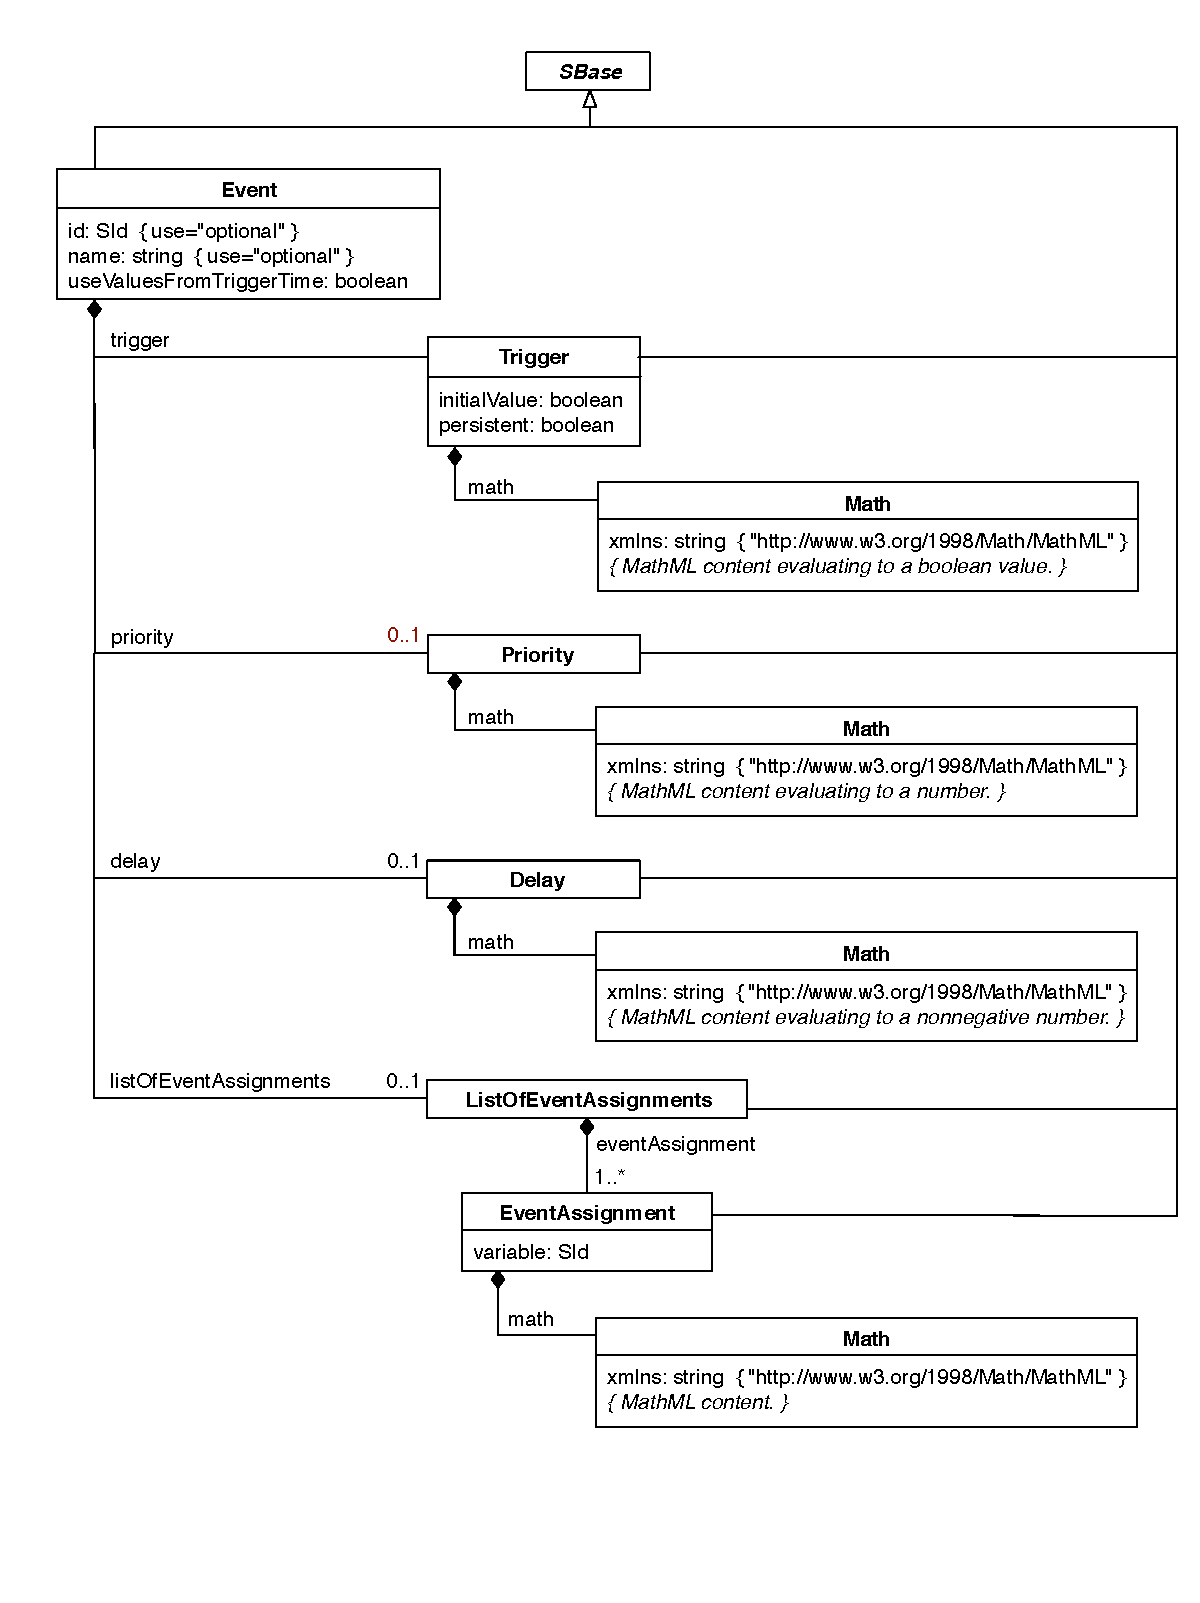
\includegraphics[scale=0.77]{figs/event-uml}
  \vspace*{-1ex}
  \caption{The definitions of \Event, \Trigger, \Delay, \Priority,
    \EventAssignment, and \ListOfEventAssignments.}
  \label{fig:event}
\end{figure}


\subsubsection{\class{Event}}

\changed{In addition to the attributes and children it inherits from \SBase,}
an \Event definition has one required attribute, \token{useValuesFromTriggerTime}
\changed{, and five optional subobjects, \Trigger, \Delay, \Priority, \ListOfEventAssignments, and \EventAssignment.}
These various features of \Event are described below.


\paragraph{The optional \token{sboTerm} attribute on \class{Event}}
\label{sec:event-sboterm}

\Event inherits an optional \token{sboTerm} attribute of type
\primtype{SBOTerm} from \SBase (see
Sections~\ref{sec:sboterm-type} and~\ref{sec:sboTerm}).  When this
attribute is present on a given \Event object instance, its value
should be an SBO identifier belonging to the branch for type
\Event indicated in Table~\ref{tab:sboterm-availability}.  The
relationship is of the form ``the event \emph{is-a} X'', where X
is the SBO term.  The term chosen should be the most precise
(narrow) one that captures the role of the event in the model.

As discussed in Section~\ref{sec:sboTerm}, SBO labels are optional
information on a model.  Applications are free to ignore
\token{sboTerm} values.  A model must be interpretable without the
benefit of SBO labels.


\paragraph{\textcolor{black}{The \token{useValuesFromTriggerTime} attribute}}
\label{sec:event-usevaluesfromtriggertime}

The possibility of defining an optional \Delay within \Event, and
the potential for multiple simultaneously-triggered events, means
there are two times to consider when interpreting an event: the
moment at which the event \emph{triggered}, and the moment at
which its assignments are \emph{executed}.  (If a \Delay subobject
is present, these moments are separated by simulation time.  If
multiple events are triggered simultaneously, these moments are
separated by the sequential execution of the event assignments.)
Similarly, it is also possible to distinguish between the moment at
which the mathematical expression of an \EventAssignment object is
evaluated, and the moment at which this value is assigned to the
entity referenced by the \EventAssignment's \token{variable}
attribute.  A model could intend the \EventAssignment expression
to be evaluated either at the moment the event is triggered, or at
the moment the event assignments are executed.  (In the former case,
a model interpreter would have to save the calculated values until
the moment of execution.)

The attribute \token{useValuesFromTriggerTime} allows a model to
indicate the moment at which the event's assignments are to be
evaluated.  A value of \val{true} indicates the values assignments
are to be computed at the moment the event is \emph{triggered}.
Conversely, \token{useValuesFromTriggerTime}=\val{false} means the
assignments are to be computed at the moment the event is
\emph{executed}.  The attribute has no default value.


\subsubsection{\class{Trigger}}
\label{sec:trigger}
\label{sec:event-trigger}

As shown in Figure~\ref{fig:event}, an \Event object \changed{may} contain
exactly one object of class \Trigger.  This object in turn must
contain two attributes, \token{persistent} and
\token{initialValue}, \changed{and may contain} a MathML \token{math} element.
The expression in the \token{math} element must evaluate to a
value of type \primtype{boolean}.  The exact moment at which this
expression evaluates to \val{true} during a simulation is taken to
be the time point when the \Event is \emph{triggered}.

An event only triggers when the expression within its \Trigger object
makes the transition in value from \val{false} to \val{true}.  The
event will trigger again at any subsequent time points when the
trigger makes the transition from \val{false} to \val{true}; in
other words, an event can trigger multiple times during a simulation
if its trigger condition makes the transition from \val{false} to
\val{true} more than once.  The behavior at the very start of
simulation time (\ie $t = 0$, where $t$ stands for time) is
determined in part by the boolean flag
\token{initialValue}, discussed below.

\begin{blockChanged}
If an instance of an \Event contains no \Trigger child, that \Event has no way of being triggered or executed in a model according to the SBML \thisLV specification.  The \Event may nevertheless be present in a model as part of (e.g.) a partially unknown system, for annotation purposes, or as part of constructs defined by an SBML Level~3 package.
\end{blockChanged}


\begin{blockChanged}
\paragraph{The \token{id} attribute on \class{Trigger}}
\label{sec:trigger-id}

\Trigger inherits an optional \token{id} attribute from \SBase, of type \primtype{SId}.  The identifier has no mathematical meaning in an SBML \thisLV model.
\end{blockChanged}


\paragraph{The \token{persistent} attribute on \class{Trigger}}
\label{sec:trigger-persistent}

In the interval between when an \Event object \emph{triggers} (\ie
its \Trigger object expression transitions in value from
\val{false} to \val{true}) and when its assignments are to be
\emph{executed}, conditions in the model may change such that the
trigger expression transitions back from \val{true} to
\val{false}.  Should the event's assignments still be made if this
happens?  Answering this question is the purpose of the
\token{persistent} attribute on \Trigger.

If the boolean attribute \token{persistent} has a value of
\val{true}, then once the event is triggered, all of its assignments
are always performed when the time of execution is reached.  The
name ``persistent'' is meant to evoke the idea that the trigger
expression does not have to be re-checked after it triggers if
\token{persistent}=\val{true}.  Conversely, if the attribute value
is \val{false}, then the trigger expression is not assumed to
persist: if the expression transitions in value back to
\val{false} at any time between when the event triggered and when it
is to be executed, the event is no longer considered to have triggered
and its assignments are not executed.  (If the trigger expression
transitions once more to \val{true} after that point, then the
event is triggered, but this then constitutes a whole new event
trigger-and-execute sequence.)

The \token{persistent} attribute can be especially useful when
\Event objects contain \Delay objects, but it is relevant even in
a model without delays if the model contains two or more events.
As explained in the introduction to this section, the operation of
all events in SBML (delayed or not) is conceptually divided into
two phases, \emph{triggering} and \emph{execution}; however, unless
events have priorities associated with them (see
Section~\ref{sec:event-priority}), SBML does not mandate a
particular ordering of event execution in the case of simultaneous
events (see Section~\ref{sec:event-semantics}).  Models with
multiple events can lead to situations where the execution of one
event affects another event's trigger expression value.  If that
other event has \token{persistent}=\val{false}, and its trigger
expression evaluates to \val{false} before it is to be executed,
the event must not be executed after all.


\paragraph{The \token{initialValue} attribute on \Trigger}
\label{sec:trigger-initialvalue}

As mentioned above, an event \emph{triggers} when the mathematical
expression in its \Trigger object transitions in value from
\val{false} to \val{true}.  An unanswered question concerns what
happens at the start of a simulation: can event triggers make this
transition at $t = 0$, where $t$ stands for time?

In order to determine whether an event may trigger at $t = 0$, it is
necessary to know what value the \Trigger object's \token{math}
expression had immediately prior to $t = 0$.  This starting value
of the trigger expression is determined by the value of the
boolean attribute \token{initialValue}.  A value of \val{true}
means the trigger expression is taken to have the value \val{true}
immediately prior to $t = 0$.  In that case, the trigger cannot
transition in value from \val{false} to \val{true} at the moment
simulation begins (because it has the value \val{true} both before
and after $t = 0$), and can only make the transition from
\val{false} to \val{true} sometime \emph{after} $t = 0$.  (To do
that, it would also first have to transition to \val{false} before
it could make the transition from \val{false} back to \val{true}.)
Conversely, if \token{initialValue}=\val{false}, then the trigger
expression is assumed to start with the value \val{false}, and
therefore may trigger at $t = 0$ if the expression evaluates to
\val{true} at that moment.

% [2010-09-09 MH] I'm thinking we should leave this for a
% document explaining the differences between L2 and L3.
%
% We note in passing that in SBML Level~2, where \Trigger lacks the
% \token{initialValue} attribute, event triggers can never
% transition from \val{false} to \val{true} at precisely $t = 0$.
% In this respect, SBML Level~2 events are similar to Level~3
% events having \token{initialValue}=\val{true}.


\paragraph{The optional \token{sboTerm} attribute on \Trigger}
\label{sec:trigger-sboterm}

\Trigger inherits an optional \token{sboTerm} attribute of type
\primtype{SBOTerm} from its parent class \SBase (see
Sections~\ref{sec:sboterm-type} and~\ref{sec:sboTerm}).  The value
given to this attribute should be an SBO identifier belonging to
the branch for type \Trigger indicated in
Table~\ref{tab:sboterm-availability}.  The relationship is of the
form ``the trigger \emph{is-a} X'', where X is the SBO term.  The
term chosen should be the most precise (narrow) one that captures
the role of the trigger in the model.

As discussed in Section~\ref{sec:sboTerm}, SBO labels are optional
information on a model.  Applications are free to ignore
\token{sboTerm} values.  A model must be interpretable without the
benefit of SBO labels.

\subsubsection{\class{Priority}}
\label{sec:event-priority}

As shown in Figure~\ref{fig:event}, an \Event object can contain
an optional \Priority subobject.  The \Priority object class, like
\Delay, is derived from \SBase and contains a MathML formula
stored in the element \token{math}.  This formula is used to
compute a dimensionless numerical value that influences the order
in which a simulator is to perform the assignments of two or more
events that happen to be executed simultaneously.  The formula may
evaluate to any \token{double} value (and thus may be a positive
or negative number, or zero), with positive numbers taken to
signifying a higher priority than zero or negative numbers.  If no
\Priority object is present on a given \Event object, no priority
is defined for that event.

\begin{blockChanged}
\paragraph{The \token{id} attribute on \class{Priority}}
\label{sec:priority-id}

\Priority inherits an optional \token{id} attribute from \SBase, of type \primtype{SId}.  The identifier has no mathematical meaning in an SBML \thisLV model.
\end{blockChanged}


\paragraph{The interpretation of priorities on events in a model}

For the purposes of SBML, \emph{simultaneous event execution} is
defined as the situation in which multiple events have identical
times of execution.  The time of execution is calculated as the
sum of the time at which a given event's \Trigger is \emph{triggered}
plus its \Delay duration, if any.  Here, ``identical times'' means
\emph{mathematically equal} instants in time.  (In practice,
simulation software adhering to this specification may have to
rely on numerical equality instead of strict mathematical
equality; robust models will ensure that this difference will not
cause significant discrepancies from expected behavior.)

If no \Priority subobjects are defined for two or more \Event
objects, then those events are still executed simultaneously but
their order of execution is \emph{undefined by this SBML
  specification}.  A software implementation may choose to execute
such simultaneous events in any order, as long as each event is
executed only once and the requirements of checking the
\token{persistent} attribute (and acting accordingly) are
satisfied.  See Section~\ref{sec:trigger-persistent} for more
information about the attribute \token{persistent}.

If \Priority subobjects are defined for two or more
simultaneously-triggered events, the order in which those particular
events must be executed is dictated by their \Priority objects,
as follows.  If the values calculated using the two \Priority
objects' \token{math} expressions differ, then the event having
the higher priority value must be executed before the event with
the lower value.  If, instead, the two priority values are
mathematically equal, then the two events must be triggered in a
\emph{random} order.  It is important to note that a \emph{random
  order is not the same as an undefined order}: given multiple
runs of the same model with identical conditions, an undefined
ordering would permit a system to execute the events in (for
example) the same order every time (according to whatever scheme
may have been implemented by the system), whereas the explicit
requirement for random ordering means that the order of execution
in different simulation runs depends on random chance.  In other
words, given two events ``A'' and ``B'', a randomly-determined
order must lead to an equal chance of executing ``A'' first or
``B'' first, every time those two events are executed
simultaneously.

A model may contain a mixture of events, some of which have
\Priority subobjects and some do not.  Should a combination of
simultaneous events arise in which some events have priorities
defined and others do not, the set of events with defined
priorities must trigger in the order determined by their \Priority
objects, and the set of events without \Priority objects must be
executed in an \emph{undefined} order with respect to each other
and with respect to the events with \Priority subobjects.  (Note
that \emph{undefined order} does not necessarily mean random
order, although a random ordering would be a valid implementation
of this requirement.)

The following example may help further clarify these points.
Suppose a model contains four events that should be executed
simultaneously, with two of the events having \Priority objects
with the same value and the other two events having \Priority
objects with the same, but different, value.  The two events with
the higher priorities must be executed first, in a random order
with respect to each other, and the remaining two events must be
executed after them, again in a random order, for a total of four
possible and equally-likely event executions: A-B-C-D, A-B-D-C,
B-A-C-D, and B-A-D-C.  If, instead, the model contains four events
all having the same \Priority values, there are 4! or 24
possible orderings, each of which must be equally likely to be
chosen.  Finally, if none of the four events has a \Priority
subobject defined, or even if exactly one of the four events has a
defined \Priority, there are again 24 possible orderings, but the
likelihood of choosing any particular ordering is undefined; the
simulator can choose between events as it wishes.  (The SBML
specification only defines the effects of priorities on \Event
objects with respect to \emph{other} \Event objects with
priorities.  Putting a priority on a \emph{single} \Event object
in a model does not cause it to fall within that scope.)

Section~\ref{sec:event-semantics} includes additional discussion
of these topics.


\paragraph{Evaluation of \class{Priority} expressions}

An event's \Priority object \token{math} expression must be
evaluated at the time the \Event is to be \emph{executed}.  During
a simulation, all simultaneous events have their \Priority values
calculated, and the event with the highest priority is selected for
next execution.  Note that it is possible for the execution of one
\Event object to cause the \Priority value of another
simultaneously-executing \Event object to change (as well as to
trigger other events, as already noted).  Thus, after executing
one event, and checking whether any other events in the model have
been triggered, all remaining simultaneous events that
\emph{either} (i) have \Trigger objects with attributes
\token{persistent}=\val{false} \emph{or} (ii) have \Trigger
expressions that did not transition from \val{true} to
\val{false}, must have their \Priority expression reevaluated.
The highest-priority remaining event must then be selected for 
execution next.  Section~\ref{sec:bp:events} provides further
discussion about implementing support for events.


\paragraph{Units of \class{Priority} object's mathematical
  expressions}

The unit associated with the value of a \Priority object's
\token{math} expression should be \token{dimensionless}.  This is
because the priority expression only serves to provide a relative
ordering between different events, and only has meaning with
respect to other \Priority object expressions.  The value of
\Priority objects is not comparable to any other kind of object in
an SBML model.


\paragraph{The optional \token{sboTerm} attribute on \class{Priority}}
\label{sec:priority-sboterm}

\Priority inherits an optional \token{sboTerm} attribute of type
\primtype{SBOTerm} from its parent class \SBase (see
Sections~\ref{sec:sboterm-type} and~\ref{sec:sboTerm}).  When a
value is given to this attribute in a \Priority instance, it
should be an SBO identifier belonging to the branch for type
\Priority indicated in Table~\ref{tab:sboterm-availability}.  The
relationship is of the form ``the priority \emph{is-a} X'', where
X is the SBO term.  The term chosen should be the most precise
(narrow) one that captures the role of the priority in the model.

As discussed in Section~\ref{sec:sboTerm}, SBO labels are optional
information on a model.  Applications are free to ignore
\token{sboTerm} values.  A model must be interpretable without the
benefit of SBO labels.


\subsubsection{\class{Delay}}
\label{sec:event-delay}

As shown in Figure~\ref{fig:event}, an \Event object can contain
an optional \Delay object.  The \Delay class is derived from
\SBase and contains a mathematical formula stored in \token{math}.
The formula is used to compute the length of time between when the
event has \emph{triggered} and when the event's assignments (see
below) are actually \emph{executed}.  If no delay is present on a
given \Event, no delay is defined for that event.

The expression in the \Delay object's \token{math} element must be
evaluated at the time the event is \emph{triggered}.  The expression
must always evaluate to a nonnegative number (otherwise, a
nonsensical situation could arise where an event is defined to
execute before it is triggered!).


\begin{blockChanged}
\paragraph{The \token{id} attribute on \class{Delay}}
\label{sec:delay-id}

\Delay inherits an optional \token{id} attribute from \SBase, of type \primtype{SId}.  The identifier has no mathematical meaning in an SBML \thisLV model.
\end{blockChanged}


\paragraph{Units of delay expressions}

The unit associated with the value of a \Delay object's
\token{math} expression should match the model's unit of
\quantity{time} (see Section~\ref{sec:model-timeUnits}).  Note
that, as in other cases of MathML expressions in SBML, units are
\emph{not} automatically predefined or assumed.  As discussed in
Section~\ref{sec:operator-arg-types}, expressions containing only
literal numbers and/or \Parameter objects without declared units
are considered to have unspecified units.  In such cases, the
correspondence between the needed entity units and the (unknown)
unit for the \Delay's \token{math} expression cannot be proven,
and while such expressions are not considered inconsistent, all
that can be assumed by model interpreters (whether software or
human) is that the units \emph{may} be consistent.

The following \Event example fragment helps illustrate this:
\label{sec:event:delay:example}

\vspace*{0.5ex}
\begin{example}
<model timeUnits="second" ...>
    ...
    <listOfEvents>
        <event useValuesFromTriggerTime="true">
            ...
            <delay>
                <math xmlns="http://www.w3.org/1998/Math/MathML">
                    <cn> 10 </cn>
                </math>
            </delay>
            ...
        </event>
    </listOfEvents>
    ...
</model>
\end{example}
\vspace*{0.5ex}

Note that the \val{<cn> 10 </cn>} within the mathematical formula
has no specified unit attached to it.  The model is not invalid
because of this, but a recipient of the model may justifiably be
concerned about what \val{10} really means.  (Ten seconds?  What
if the global unit of time on the model were changed from seconds
to milliseconds?  Would the modeler remember to change \val{10} to
\val{10$\;$000}?)  A better approach would be to declare the unit
explicitly, as in the following example:

\vspace*{0.5ex}
\begin{example}
<model timeUnits="second" ...>
    ...
    <listOfEvents>
        <event useValuesFromTriggerTime="true">
            ...
            <delay>
                <math xmlns="http://www.w3.org/1998/Math/MathML"
                      xmlns:sbml="http://www.sbml.org/sbml/level3/version2/core">
                    <cn sbml:units="second"> 10 </cn>
                </math>
            </delay>
            ...
        </event>
    </listOfEvents>
    ...
</model>
\end{example}
\vspace*{0.5ex}

While this approach will not solve the problem of updating the
value if the model's global of unit of time is changed, it will at
least inform readers of the intended duration of the delay itself
as well as make it possible for software tools to potentially
detect unit inconsistencies if the tools can perform unit
analysis.

Another, different approach is to define a global \Parameter
object for the time delay (with an appropriate unit attached), and
to replace the \token{cn} element above with a \token{ci} element
containing the parameter's identifier.  This has advantages
because \Parameter objects can have annotations and SBO terms
associated with them.


\paragraph{The optional \token{sboTerm} attribute on \class{Delay}}
\label{sec:delay-sboterm}

\Delay inherits an optional \token{sboTerm} attribute of type
\primtype{SBOTerm} from its parent class \SBase (see
Sections~\ref{sec:sboterm-type} and~\ref{sec:sboTerm}).  When a
value is given to this attribute in a \Delay instance, it should
be an SBO identifier belonging to the branch for type \Delay
indicated in Table~\ref{tab:sboterm-availability}.  The
relationship is of the form ``the delay \emph{is-a} X'', where X
is the SBO term.  The term chosen should be the most precise
(narrow) one that captures the role of the delay in the model.

As discussed in Section~\ref{sec:sboTerm}, SBO labels are optional
information on a model.  Applications are free to ignore
\token{sboTerm} values.  A model must be interpretable without the
benefit of SBO labels.


\subsubsection{\class{EventAssignment}}
\label{sec:eventassignment}
\label{sec:listofeventassignments}

\Event contains an optional element called
\token{listOfEventAssignments}, of class \ListOfEventAssignments.
In every instance of an event definition in a model, the object's
\token{listOfEventAssignments} element \changed{may have
zero or more} \token{eventAssignment} elements of class
\EventAssignment.  The object class \EventAssignment has one
required attribute, \token{variable}, and \changed{an optional} element,
\token{math}.  Being derived from \SBase, it also has all the
usual attributes and elements of its parent class.

An ``event assignment'' has effect when the event is
\emph{executed}.  (As noted above, the operation of event is
divided conceptually into two phases: the first phase when the
event is \emph{triggered} and the second phase when the event is
\emph{executed}.)  See Section~\ref{sec:event-semantics} below for
more information about events and event assignments.


\paragraph{The \token{variable} attribute}

The \changed{\EventAssignment required} attribute \token{variable} has type \primtype{SIdRef}. \changed{The value of the attribute must be the identifier of an object in the \primtype{SId} namespace of the model with mathematical meaning and the ability to be assigned.  In SBML Level~3 Core, the permitted objects classes are \Compartment, \Species, \SpeciesReference and \Parameter.  The set also includes SBML Level~3 package objects with identifiers in the \primtype{SId} namespace of the model and mathematical meaning defined to allow assignment.}

When the event is executed, the value of
the model component identified by \token{variable} is changed by
the \EventAssignment to the value computed by the \token{math}
element.  \changed{For components defined by SBML Level~3 Core, this means that} a species' quantity, species reference's
stoichiometry, compartment's size or parameter's value are reset
to the value computed by \token{math}.

Certain restrictions are placed on what can appear in
\token{variable}:
\begin{itemize}
  
\item The object identified by the value of the \token{variable}
  attribute must not have its \token{constant} attribute set 
  to \val{true}.  (Constants cannot be affected by events.)
  
\item The \token{variable} attribute must not contain the
  identifier of a reaction; \changed{in core,} only species, species references,
  compartment and parameter values may be set by an \Event.
  
\item The value of every \token{variable} attribute must be unique
  among the set of \EventAssignment objects within a given
  \Event instance.  In other words, a single event cannot have
  multiple \EventAssignment children assigning the same variable.  (All
  of them would be performed at the same time, when that
  particular \Event triggers, resulting in indeterminacy.)
  Separate \Event instances can refer to the same variable.
  
\item A variable cannot be assigned a value in an \EventAssignment
  object instance and also be assigned a value by an
  \AssignmentRule, \ie the value of the \token{variable} attribute
  in an \EventAssignment instance cannot be the same as the value
  of a \token{variable} attribute in an \AssignmentRule instance.
  (Assignment rules hold at all times, therefore it would be
  inconsistent to also define an event that reassigns the value of
  the same variable.)

\begin{blockChanged}

If the \token{variable} attribute of an \EventAssignment object references an object in an SBML namespace that is not understood by the interpreter reading a given SBML document (that is, if the object is defined by an SBML Level~3 package that the software does not support), the assignment rule must be ignored---the object's value will not need to be set, as the interpreter could not understand that package.  If an interpreter cannot establish whether a referenced object is missing from the model or instead is defined in an SBML namespace not understood by the interpreter, it may produce a warning to the user.  (The latter situation may only arise if an SBML package is present in the SBML document with a \token{package:required} attribute of \val{true}.)

\end{blockChanged}

\end{itemize}

Note that the time of assignment of the object identified by the
value of \token{variable} is always the time at which the \Event
is \emph{executed}, not when it is \emph{triggered}.  The timing
is controlled by the optional \Delay.  The time of assignment is
not affected by the \Event attribute
\token{useValuesFromTriggerTime}---that attribute affects the time
at which the \EventAssignment's \token{math} expression is
evaluated.  In other words, SBML allows decoupling the time at
which the \token{variable} is assigned from the time at which its
value expression is calculated.


\paragraph{The optional \token{sboTerm} attribute on \class{EventAssignment}}
\label{sec:eventassignment-sboterm}

\EventAssignment inherits an optional \token{sboTerm}
attribute of type \primtype{SBOTerm} from its parent
class \SBase (see Sections~\ref{sec:sboterm-type}
and~\ref{sec:sboTerm}).  When a value is given to this
attribute in a  \EventAssignment  instance, it should be an
SBO identifier belonging to the branch for type  \EventAssignment 
indicated in Table~\ref{tab:sboterm-availability}.  The relationship is
of the form ``the event assignment \emph{is-a} X'', where X is
the SBO term.  The term chosen should be the most precise (narrow)
one that captures the role of the event assignment  in the model.

As discussed in Section~\ref{sec:sboTerm}, SBO labels are optional
information on a model.  Applications are free to ignore
\token{sboTerm} values.  A model must be interpretable without the
benefit of SBO labels.


\begin{blockChanged}
\paragraph{The optional \token{id} attribute on \class{EventAssignment}}
\label{sec:eventassignment-id}

\EventAssignment inherits an optional \token{id} attribute from \SBase, of type \primtype{SId}.  The identifier has no mathematical meaning in an SBML \thisLV model.

\end{blockChanged}


\paragraph{\class{EventAssignment}'s \token{math}}

The \token{math} element contains a MathML expression that defines
the new value to be given to the object identified by the
\EventAssignment attribute \token{variable}.

As mentioned above, the time at which the expression in
\token{math} is evaluated is determined by the attribute
\token{useValuesFromTriggerTime} on \Event.  If the attribute
value is \val{true}, the expression must be evaluated when the
event is \emph{triggered}; more precisely, the values of identifiers
occurring in MathML \token{ci} \changed{elements} in the
\EventAssignment's \token{math} expression are the values they
have at the point when the event \emph{triggered}.  If, instead,
\token{useValuesFromTriggerTime}'s value is \val{false}, it means
the values at \emph{execution} time should be used; that is, the
values of identifiers occurring in MathML \token{ci} attributes in
the \EventAssignment's \token{math} expression are the values they
have at the point when the event \emph{executed}.


\paragraph{Units of the \token{math} formula in \class{EventAssignment}}

In all cases, as would be expected, the unit of measurement
associated with value of the formula contained in the \token{math}
element of an \EventAssignment object should be consistent with
the unit associated with the object identified by the
\token{variable} attribute value.  More precisely\changed{, for classes of objects defined by SBML Level~3 Core:}:
\begin{itemize}
  
\item \emph{In the case of a species}, an \EventAssignment sets
  the referenced species' quantity (\quantity{concentration} or
  \quantity{amount}) to the value determined by the formula in
  \token{math}.  The unit associated with the value produced by
  the \token{math} formula should be equal to the unit associated
  with the species' quantity.  (See
  Section~\ref{sec:species-units} for an explanation of how a
  species' quantity is determined.)

\item \emph{In the case of a species reference}, an
  \EventAssignment sets the stoichiometry of the reactant or
  product referenced by the \SpeciesReference object to the value
  determined by the formula in \token{math}.  The unit associated
  with the value produced by the \token{math} formula should be
  \token{dimensionless}, because reactant and product
  stoichiometries in reactions are dimensionless quantities.

\item \emph{In the case of a compartment}, an \EventAssignment
  sets the referenced compartment's size to the size determined by
  the formula in \token{math}.  The unit associated with the value
  produced by the \token{math} formula should be the same as that
  specified for the compartment's size.  (See
  Section~\ref{sec:compartment-units} for more.)

\item \emph{In the case of a parameter}, an \EventAssignment sets
  the parameter's value to the value of the formula in
  \token{math}.  The unit associated with the value produced by
  the \token{math} formula should be the same as parameter's
  \token{units} attribute value.
  (Section~\ref{sec:parameter-units} for more information about
  parameter units.)

\begin{blockChanged}
\item \emph{In the case of an object from an SBML Level~3 package}, an \EventAssignment sets
  the referenced object's value (as defined by that package) to the value of the formula in
  \token{math}.  The unit of measurement associated with the value produced by
  the formula should be the same as that object's \token{units}
  attribute value (if it has such an attribute), or be equal to
  the units of model components of that type (if objects of that class
  are defined by the package as having the same units).

\end{blockChanged}

\end{itemize}

Note that the formula in \token{math} has no assumed unit of
measurement associated with it.  The consistency of the units
between the formula and the entity affected by the assignment
should be established explicitly.

% \todo{someone}{explain what to do if event sets both species
% and a compartment size at same time}


\subsubsection{Example \class{Event} definitions}

The following is an example of an event.  This structure makes the
assignment $k_2 = 0$ when $P_1 \leq P_2$:

\begin{example}
<model>
    ...
    <listOfUnitDefinitions>
        <unitDefinition id="per_second">
            <listOfUnits>
                <unit kind="second" exponent="-1" multiplier="1" scale="0"/>
            </listOfUnits>
        </unitDefinition>
    </listOfUnitDefinitions>
    ...
    <listOfParameters>
        <parameter id="k2" value="0.05" units="per_second" constant="false"/>
        <parameter id="k2reset" value="0.0" units="per_second" constant="true"/>
    </listOfParameters>
    ...
    <listOfEvents>
        <event useValuesFromTriggerTime="true">
            <trigger initialValue="false" persistent="true">
                <math xmlns="http://www.w3.org/1998/Math/MathML">
                    <apply> <leq/> <ci> P_1 </ci> <ci> P_2 </ci> </apply>
                </math>
            </trigger>
            <listOfEventAssignments>
                <eventAssignment variable="k2">
                    <math xmlns="http://www.w3.org/1998/Math/MathML">
                        <ci> k2reset </ci>
                    </math>
                </eventAssignment>
            <listOfEventAssignments>
        </event>
    </listOfEvents>
</model>
\end{example}

A complete example of a model using events is given in
Section~\ref{sec:eventeg}.


\subsubsection{Detailed semantics of events}
\label{sec:event-semantics}

Any transition of a \Trigger object's \token{math} formula from
the value \val{false} to \val{true} will cause the enclosing
\Event object to \emph{trigger}.  Such a transition is not possible
at the very start of a simulation (\ie at time $t = 0$) unless the
\Trigger object's \token{initialValue} attribute has a value of
\val{false}; this defines the value of the trigger formula to be
\val{false} immediately prior to the start of simulation, thereby
giving it the potential to change in value from \val{false} to
\val{true} when the formula is evaluated at $t = 0$.  If
\token{initialValue}=\val{true}, then the trigger expression
cannot transition from \val{false} to \val{true} at $t = 0$ but
may do so at some time $t > 0$.

Consider an \Event object definition $E$ with delay $d$ in which
the \Trigger object's \token{math} formula makes a transition in
value from \val{false} to \val{true} at times $t_1$ and $t_2$.
The \EventAssignment within the \Event object will have effect at
$t_1+d$ and $t_2+d$ irrespective of the relative times of $t_1$
and $t_2$.  For example, events can ``overlap'' so that $t_1 < t_2
< t_1+d$ still causes an event assignments to occur at $t_1+d$ and
$t_2+d$.

It is entirely possible for two events to be executed
simultaneously, and it is possible for events to trigger other events
(\ie an event assignment can cause an event to trigger).  This leads
to several points:
\begin{itemize}

\item A software package should retest all event triggers after
  executing an event assignment in order to account for the
  possibility that the assignment causes another event trigger to
  transition from \val{false} to \val{true}.  This check should be
  made after each individual \Event object's execution, even when
  several events are to be executed simultaneously.  

\item Any \Event object whose \Trigger \token{persistent}
  attribute has the value \val{false} must have its trigger
  expression reevaluated continuously between when the event has
  been triggered and when it is executed.  If its trigger expression
  ever evaluates to \val{false}, it must be removed from the queue
  of events pending execution and treated as any other event whose
  trigger expression evaluates to \val{false}.

\item Although the precise time at which events are executed is
  not resolved beyond the given execution point in simulated time,
  it is assumed that the order in which the events occur \emph{is}
  resolved.  This order can be significant in determining the
  overall outcome of a given simulation.  When an event $X$
  \emph{triggers} another event $Y$ and event $Y$ has zero delay,
  then event $Y$ is added to the existing set of simultaneous
  events that are pending \emph{execution}.  Events $X$ and $Y$
  form a cascade of events at the same point in simulation time.
  An event such as $Y$ may have a special priority if it contains
  a \Priority subobject.

\item All events in a model are open to being in a cascade.  The
  position of an event in the event queue does not affect whether
  it can be in the cascade: event $Y$ can be triggered whether it
  is before or after $X$ in the queue of events pending execution.
  A cascade of events can be potentially infinite (never
  terminate); when this occurs a simulator should indicate this
  has occurred---it is incorrect for a simulator to break a
  cascade arbitrarily and continue the simulation without at least
  indicating that the infinite cascade occurred.

\item Simultaneous events having no defined priorities are
  executed in an undefined order.  This does not mean that the
  behavior of the simulation is completely undefined; merely that
  the \emph{order} of execution of these particular events is
  undefined.  A given simulator may use any algorithm to choose an
  order as long as every event is executed exactly once.  (See
  also Section~\ref{sec:event-priority}.)

\item Events with defined priorities are executed in the order
  implied by their \Priority \token{math} formula values, with
  events having higher priorities being executed ahead of events
  with lower priorities, and events with identical priorities
  being executed in a random order with respect to one another (as
  determined at run-time by some random algorithm equivalent to
  coin-flipping).  Newly-triggered events that are to be executed
  immediately (\ie if they define no delays) should be inserted
  into the queue of events pending execution according to their
  priorities: events with higher priority values value must be
  inserted ahead of events with lower priority values and after
  any pending events with even higher priorities, and inserted
  randomly among pending events with the same priority values.
  Events without \Priority objects must be inserted into the queue
  in some fashion, but the algorithm used to place it in the queue
  is undefined.  Similarly, there is no restriction on the order
  of a newly-inserted event with a defined \Priority with respect
  to any other pending \Event without a defined \Priority.  (See
  Section~\ref{sec:event-priority}.)

% [2010-09-09 MH] I don't think the following point is necessary.
% 
% \item Any event that has been executed is part of the history of
%   the model, and not part of the current state of the model.  (For
%   example, if the execution of an event with a low priority value
%   causes a different event with a higher priority to trigger and
%   immedately be executed, it is not a problem that a
%   lower-priority event executed before a higher-priority event.)

\item A model variable that is the target of one or more event
  assignments can change more than once when simultaneous events
  are processed at some time point $t$.  The model's behavior
  (output) for such a variable is the value of the variable at the
  end of processing all the simultaneous events at time $t$.

\end{itemize}


% -----------------------------------------------------------------------------
% chunks of text that maybe will be useful some day:
% -----------------------------------------------------------------------------

% Here it pays to reflect more carefully about what a reaction is.
% A reaction represents a process occurring over time.  the process
% acts on the reactants, transforming them in some way into the
% products.  the transformation may be anything from a change in
% the nature of the reactants to a simple relocation without any
% change to the nature of the reactants; for the purpose of talking
% about the speed of the reaction it does not matter.

% The ``kinetic law'' is a statement about the speed at which the
% process takes place, or more precisely, the frequency of the
% events occurring in this process.  It is by default in terms of
% moles per second, which has some intuitive appeal when dealing
% with chemical substances.  But notice that a ``mole'' is actually
% a statement about numbers of ``things'': it is 6.02e23 of whatever
% is involved.  In the case of chemical species, it is molecules of
% the substance.  To say ``one mole of'' is a shorthand way of
% saying ``6.02e23 molecules of''.  Thus, a reaction expressed as
% ``X moles per second'' is a statement that the process involves
% ``(X times 6.02e23) items per second''.

% 1 kg/sec is 1 kg/sec

% If in a reaction, the units of the species are the same as the
% reaction's substance units (default mole, redefinable by
% redefining ``substance''; sec section x), then the stoichiometries
% represent simply the ratios of the participating species: 1 mole
% of this to 2 moles of that, and so on.  If instead the species are
% given in different units, then the species quantities must be
% converted to be consistent with the units of the reaction.  Thus,
% the SBML stoichiometry may then have to incorporate a conversion:
% the stoichiometry will represent the product of the biochemical
% reaction stoichiometry and a ratio between the species substance
% and the reaction substance.

% don't forget units of reaction id


% ---

% started trying to generate the event diagram in pgf but
% it's too hard.

%   \begin{tikzpicture}[level distance=2in]
%     \node[left=1.15in,above=0.35in] (a) { \emptyClassbox{\textsl{SBase}} };
%     \node[left=0.75in] (b) {
%       \begin{classbox}{Event}
%         id: SId  \{ use="optional" \}     \\
%         name: string \{ use="optional" \} \\
%       \end{classbox} 
%     }
%     [diamond-,edge from parent fork right,grow=right,sibling distance=0.6in]
%     child {node[right=0.15in] (c) { \emptyClassbox{ListOfEventAssignments} }
%       child {node (f) {
%           \begin{classbox}{EventAssignment}
%             variable: SIdRef                                                   \\
%           \end{classbox}
%         }}
%       child {node (g) {
%           \begin{classbox}{Math}
%             xmlns: string \{ "http://www.w3.org/1998/Math/MathML" \} \\
%             \{ \emph{\mathml content} \} \\
%           \end{classbox}
%         }}
%     }
%     child {node[right=0.15in] (d) { \emptyClassbox{Delay} }
%     }
%     child {node[right=0.15in] (d) { \emptyClassbox{Trigger} }
%     }
      
% junk

%      [diamond-,edge from parent fork down,sibling distance=0.6in]
%         \begin{classbox}{Delay}
%           xmlns: string \{ "http://www.w3.org/1998/Math/MathML" \} \\
%           \{ \emph{\mathml content} \} \\
%         \end{classbox}
%       }}
%     child {node[right=0.15in] (e) {
%         \begin{classbox}{Trigger}
%           xmlns: string \{ "http://www.w3.org/1998/Math/MathML" \} \\
%           \{ \emph{\mathml content evaluating to a boolean value} \} \\
%         \end{classbox}
%       }}
%    ;
%           \begin{classbox}{EventAssignment}
%             variable: SIdRef                                                   \\
%             math: Math \{ namespace="http://www.w3.org/1998/Math/MathML" \} \\
%           \end{classbox}
%      \draw[open triangle 60-] (a) -- (b);
%      \draw node[left=0.4in,above=0.375in] {\textsf{math}};
%      \draw node[left=0.3in,below=0.225in] {\textsf{message}};
%      \draw node[left=-0.15in,below=0.215in] {\textsf{0..1}};
%  \end{tikzpicture}

%   
%   \vspace*{2ex}
%   \begin{classbox}{Trigger}
%     math: Math \{ namespace="http://www.w3.org/1998/Math/MathML" \} \\
%   \end{classbox}
%   \vspace*{2ex}
%   \begin{classbox}{Delay}
%     math: Math \{ namespace="http://www.w3.org/1998/Math/MathML" \} \\
%   \end{classbox}
%   \vspace*{2ex}
%   
